\documentclass{mimosis}

\usepackage{metalogo}
\usepackage{etoolbox}

%%%%%%%%%%%%%%%%%%%%%%%%%%%%%%%%%%%%%%%%%%%%%%%%%%%%%%%%%%%%%%%%%%%%%%%%%%%%%%%
% tabreturn additions
%%%%%%%%%%%%%%%%%%%%%%%%%%%%%%%%%%%%%%%%%%%%%%%%%%%%%%%%%%%%%%%%%%%%%%%%%%%%%%%

% warning fixes (thesis.log)
\setlength{\footheight}{20.5pt}
\setlength{\headheight}{20.5pt}
\usepackage{scrhack}
% \usepackage{lineno}\linenumbers % handy for debugging & reviews

% footnote indentation
\makeatletter
\renewcommand\@makefntext[1]{%
  \parindent 0pt%
  \noindent
  \hangindent=1.25em
  \hb@xt@1em{\hss\@makefnmark\hspace{0.1em}}#1}
\makeatother

% additional packages
\graphicspath{{./images/}}
\usepackage[toc,page]{appendix}
\usepackage[yyyymmdd]{datetime}\renewcommand{\dateseparator}{-}

% uncomment following lines to hard-code a submission date
%\month=10
%\year=2025
%\day=24

\usepackage{enumitem}
\usepackage{float}
\usepackage{forest}\useforestlibrary{edges}
\usepackage{listings}
\lstset{
  language   = Python,
  basicstyle = \small\ttfamily,
  aboveskip  = 1.5em, belowskip=1.5em, % margin
  framesep   = 0.75em,                 % padding
  frame      = lines,
  framerule  = 0.5pt,
  rulecolor  = \normalcolor
}
\usepackage{makeidx}\makeindex
\usepackage{microtype}\microtypesetup{
  activate={nocompatibility}, protrusion=false % warning fixes (thesis.log)
}
\usepackage{nameref}
\usepackage{pagecolor}
\usepackage{pgfgantt}
\usepackage{pdfpages}
%\usepackage{svg} % requires: pdflatex/latexmk -shell-escape
\usepackage{tikz}
\usepackage{xurl}

% metadata box
\usepackage{mdframed}
\newmdenv[
  topline           = false,
  rightline         = false,
  bottomline        = false,
  leftline          = true,
  linecolor         = black,
  linewidth         = 0.5pt,
  innertopmargin    = 0,
  innerrightmargin  = 0,
  innerbottommargin = 0,
  innerleftmargin   = 10pt
]{outputmeta}

% todo-notes; notes in pale blue by default
\usepackage{todonotes}
\usepackage{xcolor}
\definecolor{paleblue}{rgb}{0.7, 0.85, 1}
\definecolor{ashgray}{rgb}{0.85, 0.85, 0.85}
\definecolor{shallowblue}{HTML}{104DB0}
\definecolor{deepblue}{HTML}{051B38}
\presetkeys{todonotes}{
backgroundcolor=paleblue, bordercolor=paleblue, linecolor=paleblue}{}
\reversemarginpar
\setlength{\marginparwidth}{3cm}
\makeatletter
\renewcommand{\todo}[2][]{\@todo[caption={#2}, #1]{
  \parbox{\marginparwidth}{\renewcommand{\baselinestretch}{1.2}\small#2}
}}
\newcommand{\todoinline}[2][]{\@todo[caption={#2}, #1, inline]{#2}}
\makeatother

%%%%%%%%%%%%%%%%%%%%%%%%%%%%%%%%%%%%%%%%%%%%%%%%%%%%%%%%%%%%%%%%%%%%%%%%%%%%%%%
% commands
%%%%%%%%%%%%%%%%%%%%%%%%%%%%%%%%%%%%%%%%%%%%%%%%%%%%%%%%%%%%%%%%%%%%%%%%%%%%%%%

% build
% latexmk -r ./mimosis/mimosis-latexmkrc
% clean
% latexmk -r ./mimosis/mimosis-latexmkrc -c

%%%%%%%%%%%%%%%%%%%%%%%%%%%%%%%%%%%%%%%%%%%%%%%%%%%%%%%%%%%%%%%%%%%%%%%%%%%%%%%
% hyperlinks & bookmarks
%%%%%%%%%%%%%%%%%%%%%%%%%%%%%%%%%%%%%%%%%%%%%%%%%%%%%%%%%%%%%%%%%%%%%%%%%%%%%%%

\usepackage[%
  colorlinks = true,
  citecolor  = shallowblue,
  linkcolor  = shallowblue,
  urlcolor   = shallowblue,
  unicode,
  bookmarksnumbered,
  bookmarksdepth     = 2,
  bookmarksopen      = true,
  bookmarksopenlevel = 0
  ]{hyperref}   % tabreturn: number pdf outline
\urlstyle{same} % tabreturn: added to make the urls match the text font
\hypersetup{bookmarksdepth=2}  % tabreturn: pdf outline depth to \subsection

\usepackage{bookmark}

%%%%%%%%%%%%%%%%%%%%%%%%%%%%%%%%%%%%%%%%%%%%%%%%%%%%%%%%%%%%%%%%%%%%%%%%%%%%%%%
% bibliography
%%%%%%%%%%%%%%%%%%%%%%%%%%%%%%%%%%%%%%%%%%%%%%%%%%%%%%%%%%%%%%%%%%%%%%%%%%%%%%%

\usepackage[
  autocite     = plain,
  backend      = biber,
  doi          = true,
  url          = true,
  giveninits   = true,
  hyperref     = true,
  maxbibnames  = 99,
  maxcitenames = 99,
  sortcites    = true,
  style        = numeric,            % optional depending on bibstyle/citestyle
  bibstyle     = mimosis/acmnumeric, % tabreturn: custom .bbx file
  citestyle    = mimosis/acmnumeric  % tabreturn: custom .cbx file
]{biblatex}

%\input{mimosis/mimosis-bibliography}
% tabreturn: additional lines to swap out mimosis bibliography
\DeclareNameAlias{author}{family-given}
\newcommand{\bibliofont}{\normalfont}
\addbibresource{thesis.bib} % be sure to create symlink from chapters

%%%%%%%%%%%%%%%%%%%%%%%%%%%%%%%%%%%%%%%%%%%%%%%%%%%%%%%%%%%%%%%%%%%%%%%%%%%%%%%
% fonts
%%%%%%%%%%%%%%%%%%%%%%%%%%%%%%%%%%%%%%%%%%%%%%%%%%%%%%%%%%%%%%%%%%%%%%%%%%%%%%%

\ifxetexorluatex
  \usepackage{unicode-math}
  \setmainfont{EB Garamond}
  \setmathfont{Garamond Math}
  % load some missing symbols from another font
  \setmathfont{STIX Two Math}[%
    range = {
      \sharp,
      \natural,
      \flat,
      \clubsuit,
      \spadesuit,
      \checkmark
    }
  ]
  \setmonofont[Scale=MatchLowercase]{Source Code Pro}
\else
  \usepackage[lf]{ebgaramond}
  \usepackage[oldstyle,scale=0.7]{sourcecodepro}
  \singlespacing
\fi

%%%%%%%%%%%%%%%%%%%%%%%%%%%%%%%%%%%%%%%%%%%%%%%%%%%%%%%%%%%%%%%%%%%%%%%%%%%%%%%
% acronyms & glossary
%%%%%%%%%%%%%%%%%%%%%%%%%%%%%%%%%%%%%%%%%%%%%%%%%%%%%%%%%%%%%%%%%%%%%%%%%%%%%%%

%\newacronym[description={Principal component analysis}]
%{PCA}{PCA}{principal component analysis}
%\newacronym[description={Topological data analysis}]
%{TDA}{TDA}{topological data analysis}

%\newglossaryentry{LaTeX}{%
  %name        = {\LaTeX},
  %description = {A document preparation system},
  %sort        = {LaTeX},
%}
%\newglossaryentry{Real numbers}{%
  %name        = {$\real$},
  %description = {The set of real numbers},
  %sort        = {Real numbers},
%}

%\makeindex
%\makeglossaries

%%%%%%%%%%%%%%%%%%%%%%%%%%%%%%%%%%%%%%%%%%%%%%%%%%%%%%%%%%%%%%%%%%%%%%%%%%%%%%%
% ordinals
%%%%%%%%%%%%%%%%%%%%%%%%%%%%%%%%%%%%%%%%%%%%%%%%%%%%%%%%%%%%%%%%%%%%%%%%%%%%%%%

\makeatletter
\@ifundefined{st}{%
  \newcommand{\st}{\textsuperscript{\textup{st}}\xspace}
}{}
\@ifundefined{rd}{%
  \newcommand{\rd}{\textsuperscript{\textup{rd}}\xspace}
}{}
\@ifundefined{nd}{%
  \newcommand{\nd}{\textsuperscript{\textup{nd}}\xspace}
}{}
\makeatother

\renewcommand{\th}{\textsuperscript{\textup{th}}\xspace}

%%%%%%%%%%%%%%%%%%%%%%%%%%%%%%%%%%%%%%%%%%%%%%%%%%%%%%%%%%%%%%%%%%%%%%%%%%%%%%%
% incipit
%%%%%%%%%%%%%%%%%%%%%%%%%%%%%%%%%%%%%%%%%%%%%%%%%%%%%%%%%%%%%%%%%%%%%%%%%%%%%%%

\title{\texttt{Enhancing Python Programming Education Through Creative Computing Environments}}
\subtitle{Exploring and Developing New Python Tools for Visual Learning Contexts}
\author{Tristan Bunn}

%%%%%%%%%%%%%%%%%%%%%%%%%%%%%%%%%%%%%%%%%%%%%%%%%%%%%%%%%%%%%%%%%%%%%%%%%%%%%%%
% start
%%%%%%%%%%%%%%%%%%%%%%%%%%%%%%%%%%%%%%%%%%%%%%%%%%%%%%%%%%%%%%%%%%%%%%%%%%%%%%%

\begin{document}

\frontmatter{}
  \pagenumbering{gobble} % no page numbers until needed
  \pdfbookmark[0]{Title Page}{cover}
\newgeometry{left=2.5cm} % centering fix (for twoside)

\begin{titlepage}
  \pagecolor{deepblue} % whole page background
  \color{ashgray}      % set all text to white
  
  \vspace*{2.5cm}
  \makeatletter
  \begin{center}
    \setstretch{2.5}
    \begin{Huge}
      \@title
    \end{Huge}\\[0.8cm]
    %
    \setstretch{1.8}
    \parbox{8cm}{
      \centering
      \begin{Large}
        \@subtitle
      \end{Large}\\[0.6cm]
    }\\
    %
    \emph{by}\\
    \textbf{\@author}
    %
    \vfill
    \emph{under the supervision of}\\
    Dr Aaron Bere\\
    Dr Michelle Douglas
    \vfill
    A document submitted in partial fulfillment of the requirements for the degree of\\
    \textsc{Doctor of Philosophy}\\
    at\\
    %\textsc{Torrens University Australia}\\
    \bigskip
    \includegraphics[width=3.5cm]{frontmatter/torrens-university-australia-logo}\\
    \monthname\space\the\year
  \end{center}
  \makeatother
\end{titlepage}

% reset page background + text color
\nopagecolor
\color{black}
\restoregeometry % centering fix

% ashgray page
\pagecolor{ashgray}\null\thispagestyle{empty}
\clearpage
\nopagecolor % reset back to white for following pages

\cleardoublepage

  %\pdfbookmark[0]{CHANGELOG}{changelog}
\begingroup
\color[HTML]{777777}\small

\textit{\large{build: \today{}--\currenttime{}}}\bigskip

\textbf{CHANGELOG}\bigskip{}

\textit{2025-01-01}
\begin{itemize}
\item Final word count: ... % texcount -inc thesis.tex
\item ...
\end{itemize}

\endgroup

  \pagenumbering{roman}\setcounter{page}{1} % start roman numbering
  \chapter{Declaration of Originality}

This thesis is my own work, and to the best of my knowledge, it contains no materials previously published or written by another person, and no materials which have been accepted for the award of any other degree or diploma at Torrens University Australia or any other institution, except where I have made due acknowledgement. I acknowledge that copyright of published work contained within this thesis resides with the copyright holder(s) of those works. Any contribution made to the research by others is explicitly acknowledged.

\section*{Use of Generative AI}

I have used AI-assisted tools to support the preparation of this thesis. Specifically, I employed Grammarly~\cite{grammarly_inc_grammarly_2025} extensively for proofreading and editing, and ChatGPT (OpenAI)~\cite{openai_inc_chatgpt_2025} and Claude (Anthropic)~\cite{anthropic_pbc_claude_2025} to scaffold parts based on my drafts and to assist with summary sections. In combination with Grammarly, I also used these large language models to refine, condense, and improve the clarity of some language. I confirm that I restricted the use of these tools to my draft text, avoiding any submission of sensitive research data or participant information. All intellectual contributions, interpretations, analyses, and arguments remain my own, except where I have made due acknowledgement. Moreover, I reviewed any AI output to verify, critically examine, and refine it before any integration into the thesis content.

\bigskip

\begin{figure}[h]
\includegraphics[width=6cm]{frontmatter/signature}
\end{figure}

Tristan Alan Bunn | \today

  \chapter{Authority of Access Statement}

I authorise Torrens University Australia, and any library with which it has a formal agreement, to archive my thesis and to make hardbound and digital copies available through the Library. These copies may be loaned, copied, or communicated in any form of media, whether currently known or developed in the future, subject to the provisions of the \textit{Copyright Act 1968}. I retain the right to use all or part of this thesis in future works.

\bigskip

\begin{figure}[h]
\includegraphics[width=6cm]{frontmatter/signature}
\end{figure}

Tristan Alan Bunn | \today

  \chapter{Ethical Conduct Statement}

The research associated with this thesis was conducted in accordance with the \textit{National Statement on Ethical Conduct in Human Research} (2023).

\bigskip

\begin{figure}[h]
\includegraphics[width=6cm]{frontmatter/signature}
\end{figure}

Tristan Alan Bunn | \today

  \chapter{Abstract}

%\todoinline{\textit{Thesis must include an extended abstract of no more than 500 words; this abstract is shared with potential examiners, so must offer a clear summary of all aspects of the thesis.}}

Traditional approaches to teaching programming fundamentals often pose barriers for learners whose primary orientation is artistic- or design-focused. This thesis investigates Python-based creative computing environments as a solution, evaluating existing tools and developing new software and techniques for visual learning contexts, with a focus on students in creative and interdisciplinary fields.

The thesis adopts a hybrid folio/thesis-by-publication format, encompassing software development, scholarly publications, presentations, learning resources, and creative works. Collectively, these outputs demonstrate scholarly contribution, active community engagement, and the artistic applications of novel programming practices.

A central contribution is the creation of Thonny-py5mode, a plugin that integrates the py5 library into the Thonny IDE, serving as a contemporary successor to Processing's discontinued Python Mode (Processing.py). It enables learners to generate graphical and interactive output by writing Python code, bridging technical concepts with creative exploration. An empirical evaluation applies the Task--Technology Fit framework to assess Thonny-py5mode, surveying 143 students in an introductory Python course and analysing their responses with Structural Equation Modelling (SEM) to capture factors influencing user adoption in educational contexts.

The thesis also considers the emerging role of generative AI in programming education. While acknowledging its benefits, it highlights risks of over-reliance and proposes graphical task design with Thonny-py5mode as a strategy to mitigate GenAI misuse. As a relatively late addition, this strand of inquiry foregrounds future research directions and underscores the continuing evolution of the field.

This research demonstrates how Python tools and purpose-built environments, supported by targeted curricula, can lower barriers to programming education by employing graphical and multimedia output to enhance student engagement, conceptual understanding, and motivation.

  \chapter{Acknowledgements}

I want to express my sincere gratitude to my supervisors, Dr Michelle Douglas and Dr Aaron Bere, for their invaluable guidance and support, crucial to the successful transition to and completion of my PhD at Torrens University Australia. Also, thank you to TUA for supporting my studies.

I extend my heartfelt thanks to my initial (Victoria University of Wellington) supervisors, Dr Craig Anslow and Dr Karsten Lundqvist, for their excellent guidance in preparing my successful research proposal and seeing me through to full PhD candidature. 

I am profoundly grateful to the creators, maintainers, and community surrounding Processing, particularly its Python-related projects, py5 and Processing.py. Your efforts have significantly enriched educational and creative coding communities, inspiring my students and me. 

Also, a special thank you to all those whose support and collaboration assisted in completing and disseminating the publications, presentations, and creative works contained herein---this includes funding bodies and sponsors, editors and peer reviewers, study participants, conference and exhibition organisers, and the publishers and academic platforms that provided opportunities to present and share this work with a broader audience.

%\textcolor{white}{Finally, to the PBRF: thank you for exemplifying how research assessment mechanisms can entrench exclusivity, ensuring that those outside the preferred networks remain undervalued.}

\subsection*{Technical Details and Credits}
I have typeset this document using a modification of the \textit{Mimosis} \LaTeX\ template, available at \url{https://github.com/Pseudomanifold/latex-mimosis}. I have prepared all vector graphics (multiple diagram figures) using Inkscape.


  \tableofcontents{}\addcontentsline{toc}{chapter}{Contents}
  \listoffigures{}\addcontentsline{toc}{section}{List of Figures}
  \listoftables{}\addcontentsline{toc}{section}{List of Tables}

\mainmatter

  %\part[A good part]{%
    %A good part\\
    %%
    %\vspace{1cm}
    %%
    %\begin{minipage}[l]{\textwidth}
    %%
    %\textnormal{%
      %\normalsize
      %%
      %\begin{singlespace*}
        %\onehalfspacing
        %%
        %You can also use parts in order to partition your great work
        %into larger `chunks'. This involves some manual adjustments in
        %terms of the layout, though.
      %\end{singlespace*}
    %}
    %\end{minipage}
  %}

  \chapter{Introduction}
\label{chap:introduction}

Students studying creative computing, creative technologies, and related fields benefit from learning computer programming in various ways. Firstly, programming expands creative possibilities by enabling more interactive and dynamic work, while also providing the ability to customise or even build entirely new digital tools, removing the constraints of `off-the-shelf' software~\cite{shiffman_learning_2008}. It also supports interdisciplinary practice, equipping students to contribute effectively to projects that merge art, design, technology, and science~\cite{greenberg_processing_2016}. Beyond enhancing creativity, programming education fosters industry-relevant capabilities; graduates who possess coding skills can pursue diverse roles in areas such as visual effects, video games, virtual reality, and interactive media~\cite{carey_skills_2019}. Additionally, literacy in different coding languages can facilitate better collaboration by bridging the gap between artists, developers, and technical specialists, leading to more cohesive and effective project outcomes~\cite{davis_role_2006}.

\textit{Creative computing} refers to the use of computer science and programming as media for creativity, employing algorithms, code, and computational processes to generate digital works such as interactive installations, generative art, or digital music. \textit{Creative technology}, by contrast, highlights the application of emerging platforms and tools that extend traditional artistic practices and enable new forms of hybrid or physical expression, such as virtual and augmented reality, 3D printing, sensors, or wearable devices. Both fields sit at the intersection of art, technology, and human innovation, and both prepare students for rapidly evolving creative industries. While one often encounters the terms used interchangeably, the distinction lies in emphasis: creative computing foregrounds computational techniques as a medium of expression, whereas creative technology foregrounds tools and platforms that expand the possibilities of creative practice~\cite{smu_meadows_school_of_the_arts_differences_2023}.

This study focuses on the pedagogical aspects of creative computing and creative technologies practice---specifically, the approach to programming education that emphasises creating multimedia outputs. Such methods typically employ creative coding and art- or design-oriented curricula and teaching methodologies, often aimed at students in creative fields but also applicable to those in other domains~\cite{yee-king_examining_2020}.

More specifically, this thesis explores Python-based creative computing environments (tools and other software) for education. Python, a high-level programming language, has gained significant prominence due to its simplicity, readability, and versatility~\cite{thomas_pragmatic_2019}. Initially developed by Guido van Rossum and released in 1991, Python's design philosophy emphasises code readability and clear syntax, allowing programmers to express concepts in fewer lines of code than C++ or Java. This efficiency and a comprehensive standard library have made Python a favoured choice among developers across various fields~\cite{processing_foundation_overview_2022}. As the forthcoming chapters demonstrate, the Python language's versatility extends beyond conventional software development, finding substantial applications in creative computing.

In summary, this PhD investigates innovative approaches to enhancing Python programming education by integrating, expanding, and developing new creative computing tools (software) and techniques (creative coding practice). It includes the development of tailored curricula, comprehensive documentation, and a sole-authored book. 

Grounded in peer reviewed journal articles (Quartile 2 or higher), the thesis explores and evaluates the effectiveness of Python-based educational environments and creative coding techniques through empirical research methods. Additionally, artistic works showcased at prominent venues illustrate these tools and techniques' practical applications and creative potential. Findings and insights are further disseminated through presentations at esteemed academic and professional conferences, promoting broader awareness and adoption of these advancements in programming education.

\section{Thesis Presentation}

This PhD thesis employs a hybrid structure combining elements of (primarily) a \textbf{Folio of Advanced Professional Practice} and (secondarily) a \textbf{Thesis by Publication}, as defined in the \textit{Higher Degree by Research Thesis Guidelines}\footnote{~TUA Higher Degree by Research Thesis Guidelines at \url{https://torrens.blackboard.com/bbcswebdav/xid-44216710_1}} set forth by Torrens University Australia. 

The elected format allows for a comprehensive exploration of the PhD topic and new development (and testing) of innovative methods in Python creative computing through bespoke software development, scholarly publications, presentation outputs, and creative works---all completed during the PhD enrolment, which commenced in October 2019 (Appendix \ref{appendix:vuw-candidature}), and forming a coherent and thematic research narrative. This collection of outputs forms the core of the folio, with each marking a significant milestone in the research journey. Collectively, they contribute to the academic discourse surrounding Python programming education that employs creative computing environments, addressing existing gaps in the literature while proposing novel solutions to contemporary pedagogical challenges.

For the reader's convenience, this thesis organises the outputs by type (\nameref{chap:publications}, \nameref{chap:presentation-outputs}, \nameref{chap:creative-works}) and, within each grouping, presents the contents in chronological order to illustrate the research's evolution over time. Where practical and necessary, each output is presented in full, prefaced by a concise introduction that situates it within the broader research narrative. These works span various stages of inquiry, from initial exploration and hypothesis development to detailed studies and practical applications. Central themes are consistently revisited through diverse methodologies and analytical frameworks, reinforcing the study's contributions.

\subsection{Chapter Structure}

This outline provides a high-level summary of the chapters comprising this PhD thesis, using concise chapter descriptions and a diagram (Figure~\ref{fig:thesis-overview}) to offer a conceptual overview of the entire document's contents. The elected structure facilitates a thorough understanding of the core concepts and research journey, and includes dedicated chapters that group folio outputs. Moreover, it accommodates the study's practical implications, significance, limitations, and discussion on potential future directions.

\begin{figure}[htbp]
  \centering
  \setstretch{0.7}
  \begin{forest}
  for tree={
    align=left,
    anchor=west,
    calign=first,
    child anchor=west,
    draw=none, % no cell outlines
    font=\footnotesize,
    forked edges,
    grow'=east,
    l sep=1cm,
    parent anchor=east
  }
  [, phantom
    [\ref*{chap:introduction}.~~\nameref*{chap:introduction}, fill=red!20]
    [\ref*{chap:literature-review}.~~\nameref*{chap:literature-review}, fill=blue!20
      [\nameref{sec:creative-coding-software}, fill=blue!20]
    ]
    [\ref*{chap:software}.~~\nameref*{chap:software} (Thonny-py5mode and accompanying documentation), fill=green!20]
    [\ref*{chap:publications}.~~\nameref*{chap:publications}, fill=orange!30
      [\nameref{sec:no-starch} {[No Starch Press 2021]}, fill=orange!30]
      [\nameref{sec:mtap} {[MTAP 2024]}, fill=orange!30]
      [\nameref{sec:jise} {[JISE 2025]}, fill=orange!30]
    ]
    [\ref*{chap:presentation-outputs}.~~\nameref*{chap:presentation-outputs}, fill=gray!30
      [\nameref{sec:processing.py-creative-coding-with-python} {[Kiwi PyCon X (2019)]}, fill=gray!30]
      [\nameref{sec:processing-python-mode-for-creative-coding-and-teaching} {[Libre Graphics Meeting 2020]}, fill=gray!30]
      [\nameref{sec:creative-coding-with-python-and-processing} {[CC Fest 2021]}, fill=gray!30]
      [\nameref{sec:novel-visualisations-with-python-and-p5} {[Outlier 2021]}, fill=gray!30]
      [\nameref{sec:thonny-+-py5-a-python-3-environment-for-processing} {[Processing Community Day (2021)]}, fill=gray!30]
      [\nameref{sec:generate-svg-for-pen-plotters-using-python} {[CC Fest 2022]}, fill=gray!30]
      [\nameref{sec:demystifying-the-python-processing-landscape-an-overview-of-tools-combining-python-and-processing} {[SIGGRAPH 2022]}, fill=gray!30]
      [\nameref{sec:generative-art-with-python-using-py5-and-bpy} {[PyCon XI (2022)]}, fill=gray!30]
      [\nameref{sec:blender-scripting-for-creative-coding-projects} {[SIGGRAPH Asia 2022]}, fill=gray!30]
      [\nameref{sec:mitigating-ai-misuse-in-introductory-python-courses-with-graphical-programming-tasks} {[PyCon 2025]}, fill=gray!30]
    ]
    [\ref*{chap:creative-works}.~~\nameref*{chap:creative-works}, fill=pink!40
      [\nameref{sec:the-end-of-random-seed} {[exhibited at Between 2021]}, fill=pink!40]
      [\nameref{sec:north} {[exhibited at ADA Network Symposium 2021]}, fill=pink!40]
      [\nameref{sec:south} {[exhibited at Link Conference 2021]}, fill=pink!40]
      [\nameref{sec:relics-u130c8} {[exhibited at Motyf 2022]}, fill=pink!40]
      [\nameref{sec:digital-aquatics} {[published in Processing Community Catalog (2023)]}, fill=pink!40]
    ]
    [\ref*{chap:conclusion}.~~\nameref*{chap:conclusion}, fill=cyan!20
      [\nameref{sec:contribution-to-knowledge}, fill=cyan!20]
    ]
  ]
  \end{forest}
  \vspace{1mm}\caption{Overview of thesis contents and structure}
  \label{fig:thesis-overview}
\end{figure}

\paragraph{\ref{chap:introduction}.~~\nameref{chap:introduction}}
(current chapter) Introduces the thesis by outlining the content structure and describing its context, scope, and significance. It lists the research objectives and questions, laying the groundwork for the key themes explored in subsequent chapters, and provides an introduction to creative coding, programming education, and Python.

\paragraph{\ref{chap:literature-review}.~~\nameref{chap:literature-review}}
Identifies gaps in current research and tools related to creative computing and Python programming education, positioning the work within the broader academic discourse. Given the folio/publication-based framing of this thesis, and to avoid repetition, the literature is distributed across the \nameref{chap:publications} (as part of the journal articles), the \nameref{chap:presentation-outputs}, and, to a lesser extent, the \nameref{chap:creative-works} chapter.

\paragraph{\ref{chap:software}.~~\nameref{chap:software}}
Covers the Thonny-py5mode plugin, outlining its key features, supporting documentation, and the development process, including associated funding and recognition. The \textit{\nameref{sec:jise}} article complements this chapter by detailing the plugin's technical implementation and design rationale. \nameref{chap:publications}, \nameref{chap:presentation-outputs}, and \nameref{chap:creative-works} assess the software's effectiveness and its contribution to the research objectives, while also demonstrating its practical applications and broader capabilities.

\paragraph{\ref{chap:publications}.~~\nameref{chap:publications}}
Presents the collected manuscripts---comprising a sole-authored book and peer reviewed articles published in Q1 and Q2 journals---that together form the scholarly core of the thesis. These works explore both new and existing tools, techniques, and curricula for Python-based creative computing, including results of the user studies conducted as part of this research.

\paragraph{\ref{chap:presentation-outputs}.~~\nameref{chap:presentation-outputs}}
Documents each presentation accompanied by an introduction that outlines its contribution to the thesis and integration into the overall research narrative. Delivered at prominent gatherings, the topics encompass innovative tools, creative coding practices, and teaching methodologies in Python programming that emphasise a focus on creative computing.

\paragraph{\ref{chap:creative-works}.~~\nameref{chap:creative-works}}
Presents a series of creative works developed using Python-based creative coding tools and techniques explored throughout this PhD research. These works have been exhibited at various online and in-person events and featured in published outputs.

\paragraph{\ref{chap:conclusion}.~~\nameref{chap:conclusion}}
Consolidates the research findings, tools, publications, presentations, and creative works, demonstrating how they collectively advance Python programming education through creative computing. Specifically, it highlights the interconnections among these outputs and their broader implications for educational practice, summarises the key findings, articulates the thesis' \nameref{sec:contribution-to-knowledge}, and reflects on the strengths and limitations of the developed tools and techniques. The chapter concludes by outlining future research directions and opportunities for further innovation in Python-based creative computing environments.

\paragraph{\hyperref[appendix:start]{Appendices}}
Collects supplementary material supporting the thesis, including ethics clearance, folio evidence, survey forms, anonymised data, code samples, and other relevant resources. Where applicable, chapter content will cite resources contained within the appendices.

\subsection{A Note on Methodology}

Notably, this thesis does not include a dedicated Methods or Methodology chapter. Following thesis-by-publication conventions, each output in the \nameref{chap:publications} and \nameref{chap:presentation-outputs} chapters---and, to a lesser extent, the \nameref{chap:creative-works} chapter---details its respective method(s)~\cite{denholm_supervising_2007}. The PhD folio is interdisciplinary in nature, spanning digital technology, education, and creative practice across multiple output types. Such a scope necessitates varied methodological framings~\cite{robins_phd_2008}. Accordingly, the thesis situates its methods within the development process rather than fixing them in advance. A linking commentary and concluding chapter synthesise the diverse strands, articulating the evolution of the PhD process as a whole. Moreover, the structure avoids repetition and supports the coherence of the folio/publication thesis format.

\section{Research Context and Significance}
\label{sec:research-context-and-significance}

This PhD argues that an increasing convergence of art, design, and technology has amplified the need for robust programming education tailored to creative disciplines. As technology continues to permeate facets of creative work, the ability to program is a valuable skill that can expand creative boundaries, facilitate interdisciplinary collaboration, and open doors for graduates entering emerging industries. However, teaching programming to students within creative fields can present unique challenges~\cite{carey_skills_2019, davis_role_2006, shiffman_learning_2008}. Creative computing offers a promising approach that invites learners to merge computational thinking with artistic and design-based expression.

Software applications like the Processing\footnote{~\url{https://processing.org}} IDE (Integrated Development Environment) provide creative computing environments for writing code in Java and other languages. While older versions of the Processing IDE can accommodate Python, work on this aspect is now discontinued and ``Python Mode'' (Processing.py) will not operate correctly in current versions. 

Python is a widely used programming language known for its simplicity and versatility~\cite{kaila_changing_2023}; this thesis argues that there remains significant potential for developing new Python-based tools and pedagogical approaches---akin to Processing's---that make coding more accessible, engaging, and aligned with the goals of learners pursuing foundational programming education for eventual entry into creative industries. 

Figure~\ref{fig:venn-positioning} illustrates how this PhD is positioned at the convergence of Creative Coding, Programming Education, and Python. 

\begin{figure}[htbp]
\centering
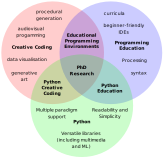
\includegraphics[width=0.7\textwidth]{chapters/chapter01-introduction/venn-positioning}
\captionsetup{width=0.7\textwidth}
\caption{Venn diagram positioning this PhD research. Figure by the author.}
\label{fig:venn-positioning}
\end{figure}

The PhD focus is developing new tools, curricula, and methods that offer students in creative (and even other) disciplines an approachable way to learn \textit{textual programming}\footnote{~Textual programming involves typing lines of code instructing computers to perform tasks} through coding graphical and interactive outputs using Python. As illustrated in Figure~\ref{fig:venn-context}, the research examines the topic from three principal angles:

\begin{figure}[htbp]
\centering
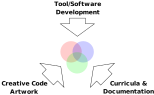
\includegraphics[width=0.7\textwidth]{chapters/chapter01-introduction/venn-context}
\captionsetup{width=0.7\textwidth}
\medskip\caption{Contextualising this PhD research approach. Figure by the author.}
\label{fig:venn-context}
\end{figure}

\begin{enumerate}

\item{\textbf{Tool/Software Development}:} 
Focussing on creating, integrating, and refining Python-based tools, notably the Thonny-py5mode plugin, developed as part of this research to facilitate creative coding practices. Thonny-py5mode is designed to align with the needs of creative disciplines, enabling seamless integration of Python code into artistic processes. Its development emphasises usability and accessibility, striving to accommodate students from varying technical backgrounds to engage with code through programming multimedia outputs.

\item{\textbf{Curricula \& Documentation}:} 
Involving designing new educational materials and curricula tailored to programming education for creative disciplines; this includes comprehensive texts---a sole-authored book and web-based software tutorials---that promote a hands-on, exploratory learning experience aimed at producing graphical and interactive output using Python code. The goal is to bridge the gap between technical programming concepts and creative practice, accommodating a learning environment where students can apply programming in meaningful, artistic contexts.

\item{\textbf{Creative Code Artwork}:} 
Exploring the application of Python-based tools and techniques through the creation of digital art and interactive media, including original artworks exhibited at events and in published catalogues. These demonstrate the potential of the environments and tools explored and developed as part of this research, while also showcasing how programming can inspire creative project outcomes.

\end{enumerate}

The significance of this study lies in its potential to influence programming education for creative fields. It contributes to the growing body of knowledge in creative computing pedagogy, providing educators with new strategies and tools to enhance student engagement and learning outcomes. Moreover, the practical implications of this research extend beyond the classroom, as the tools and techniques developed here can offer new ways to produce code-generated output for a broad range of creative applications, including digital art, design, interactive media, and entertainment.

The subsections that follow provide an essential introduction to \nameref*{sec:intro-creative-coding}, \nameref*{sec:intro-programming-education}, and \nameref*{sec:intro-python}, as contextualised within this PhD. These topics are explored in greater detail in the \nameref{chap:literature-review} chapter, as well as through the outputs presented in the \nameref{chap:publications}, \nameref{chap:presentation-outputs}, and \nameref{chap:creative-works} chapters.

\subsection{Creative Coding}
\label{sec:intro-creative-coding}

Creative coding spans applications like generative art, motion graphics, live coding performances, interactive installations, wearables, and robotics. In education, it engages students in programming through hands-on, interdisciplinary projects that blend art, design, and technology. This approach encourages curiosity, lowers the fear of failure, and makes coding more accessible by connecting it to visual, auditory, and tactile experiences~\cite{bown_creative_2020, caravati_interfacing_2024}.

It is common in creative coding to refer to programs as ``sketches,'' especially within Processing environments. This terminology originates from an analogy with visual arts, where a sketch refers to a rough, initial drawing meant to explore ideas. Processing (created by Casey Reas and Ben Fry in 2001) officially adopted this term (Figure~\ref{fig:processing-ide}) to reflect that coding should be experimental and iterative, much like drawing a sketch~\cite{reas_processing_2014}. 

\begin{figure}[htbp]
\centering
\includegraphics[width=0.8\textwidth]{chapters/chapter01-introduction/processing-ide}
\captionsetup{width=0.8\textwidth}
\caption{Screenshot of the Processing 4.3 IDE. Note the use of ``Sketch'' within the interface. Screenshot by the author.}
\label{fig:processing-ide}
\end{figure}

This aligns with the philosophy of Processing, which encourages users---especially artists and designers---to approach programming with a creative, low-stakes mindset. The term ``sketch'' is used in other creative coding tools and frameworks, including p5.js (a JavaScript version of Processing) and Arduino (microcontroller programming).

Creative coding emphasises creative outcomes over abstract syntax, attracting learners not typically drawn to computer science while engaging students across art, music, and design (and also computing \& information sciences)~\cite{mcnutt_study_2023, wing_computational_2006}. Its adaptability and emphasis on exploration provide an inclusive framework for programming education, supporting varied learning pathways and modes of skill development~\cite{urban_arts_creative_2023}. In addition to introducing core technical skills, creative coding can offer several other benefits:

\paragraph{Engagement and Motivation} Research affirms that creative coding environments can increase student engagement and motivation by situating programming within contexts that feel meaningful and enjoyable. Walsh \textit{et al.} demonstrate how combining craft with block-based coding in Scratch encourages sustained interest and playful exploration~\cite{walsh_crafting_2022}. Dufva highlights how frameworks such as Processing and Arduino stimulate intrinsic motivation by reframing code as a form of creative expression~\cite{dufva_creative_2021}. These findings support broader claims that creative coding projects make the process of learning programming more enjoyable and encouraging~\cite{mccarthy_getting_2015}.

\paragraph{Inclusivity and Appeal to Underrepresented Groups}  
Research increasingly shows that creative coding contexts can broaden participation by engaging groups historically underrepresented in computing. Walsh \textit{et al.} found that arts-integrated coding activities promoted inclusivity among underserved urban youth~\cite{walsh_crafting_2022}; Dufva emphasises feminist and critical approaches that frame coding as a cultural and political practice rather than a purely technical skill~\cite{dufva_creative_2021}. Prominent creative coding communities explicitly promote diversity and inclusion~\cite{long_coding_2023}, such as The Processing Foundation, whose mission statement directly highlights these values~\cite{processing_foundation_processing_2024}.

\paragraph{Lowering Barriers to Entry} Simplified, beginner-friendly environments lower the threshold for participation by reducing technical overhead~\cite{walsh_crafting_2022}. Dufva situates Processing and Arduino as accessible platforms for experimenting with art and code~\cite{dufva_creative_2021}, complementing findings that such environments avoid complex setup, while simultaneously providing a pathway between novice and professional developer tools with features like autocomplete and debugging functionality, thereby facilitating a smoother transition to industry-standard practices and coding environments~\cite{mccarthy_getting_2015,processing_foundation_overview_2022}.

\paragraph{Code Exploration Through Art} Creative coding highlights the intersection of programming, art, and design. As Dufva demonstrates, this bridges a gap between programming and art education, facilitating playful experimentation through live coding, code poetry, and maker practices~\cite{dufva_creative_2021}. Similarly, Walsh \textit{et al.} highlight how students integrated hand-crafted characters into Scratch games, blurring boundaries between craft and computation~\cite{walsh_crafting_2022}. Tools like number sliders and colour pickers encourage inventive tinkering, helping students to intuitively discover new ideas while still writing textual code~\cite{van_rossum_variables_2023}. Some environments, such as Hydra and Visor (Figure~\ref{fig:visor-ide}), include REPL characteristics, providing rapid feedback in response to code edits and additions. Code is entered and executed piecewise in a REPL (read--eval--print loop), meaning the output updates without rerunning the entire program~\cite{jack_documentation_2022, purvis_cjing_2019}.

\begin{figure}[htbp]
\centering
\includegraphics[width=1.0\textwidth]{chapters/chapter01-introduction/visor-ide}
\caption{Visor is a live coding environment for real-time visual performance, bridging the gap between creative coding and VJing. Screenshot from Jack Purvis (2024). Source:~\cite{purvis_visor_2024}.}
\label{fig:visor-ide}
\end{figure}

\paragraph{Building Confidence and Reducing Frustration} Evidence suggests that creative coding builds learner confidence by providing observable, incremental successes and reducing common frustrations, helping maintain learner momentum and reinforcing a sense of accomplishment~\cite{cc2020_task_force_chapter_2021}. Walsh \textit{et al.} found that students reluctant to engage with coding gained confidence through hybrid craft--code projects, while those already interested developed patience and creativity~\cite{walsh_crafting_2022}. Dufva similarly reports that hands-on, low-stakes assignments (e.g., ``human fax machine'' sound-to-drawing tasks) helped students reframe coding as accessible and culturally relevant~\cite{dufva_creative_2021}. Static analysis tools (e.g., linting) and auto-formatting in creative coding environments help students avoid common errors and maintain organised code. Simplified syntax and libraries lower entry barriers, while supportive communities offer resources and guidance to help overcome challenges~\cite{processing_foundation_overview_2022}.

In summary, creative coding offers a dynamic and inclusive approach to programming education that resonates with diverse learners and transcends traditional coding paradigms. Beginner-friendly tools like Processing and p5.js, coupled with supportive communities, foster confidence and inclusivity. This PhD aims to combine these benefits with bespoke Python-based tools and pedagogy.
    
\subsection{Programming Education}
\label{sec:intro-programming-education}

Programming education has long incorporated visual and interactive elements to enhance student engagement and understanding. Turtle graphics, commonly used in computer education during the 1980s and closely associated with the Logo programming language, provided an engaging way for children to interact with programming concepts through visual feedback~\cite{abelson_turtle_1981}.

Developed by Seymour Papert, Cynthia Solomon, and Wallace Feurzeig, Logo's Turtle graphics allowed children to visualise abstract programming ideas by controlling an on-screen ``turtle'' to draw shapes and patterns. This embodied Papert's \textit{constructionist} learning theory: learning by making, where students build knowledge through actively constructing projects. This simple yet powerful approach sought to make coding more accessible and enjoyable, promoting problem-solving skills in a creative way. Over time, Turtle graphics evolved through various versions and adaptations of Logo~\cite{solomon_history_2020}.

Python's standard library includes a Turtle graphics module inspired by Logo's. The module allows users to control turtles in a 2D space (Figure~\ref{fig:python-turtle}) and remains a popular tool for beginners to learn programming fundamentals using Python's syntax and data structures~\cite{nanavati_pythons_2020, vidal_duarte_when_2017}.

\begin{figure}[htbp]
\centering
\includegraphics[width=0.8\textwidth]{chapters/chapter01-introduction/python-turtle}
\captionsetup{width=0.8\textwidth}
\caption{A simple square drawn using Python's Turtle graphics library, demonstrating basic commands for movement and rotation. Screenshot by the author.}
\label{fig:python-turtle}
\end{figure}

Processing was among the first programming environments explicitly developed for creatives---artists, designers, and others in related fields---emphasising accessibility to programming as a medium for visual expression. Unlike many earlier programming environments focused on visual output, Processing was purpose-built to meet the creative community's needs, streamlining the process of transforming artistic concepts into code and, ultimately, code into multimedia outputs~\cite{reas_modern_2018}.

Several Processing variants have appeared since the release of the (Java-based) original, each designed to extend the Processing concept into different programming environments and languages, including p5.js (JavaScript), JRubyArt (Ruby), and Processing.py (the now outdated Python mode), among others~\cite{wikipedia_processing_2025}.

Processing has significantly impacted programming education, inspiring learners to see coding as a technical skill \textit{and} a medium for creative expression. There is a wealth of books, reference materials, and resources available for Processing and its variants, making it one of the most well-documented creative coding initiatives. As of writing, the Processing website lists 36 books covering topics from programming generative art to data visualisation, many with an introductory programming focus~\cite{processing_foundation_books_2024}. 

Several educational websites use Processing environments to teach programming fundamentals, often within a creative coding context, including 
\href{https://thecodingtrain.com}{The Coding Train}, \href{http://funprogramming.org}{Fun Programming},
\href{https://happycoding.io}{Happy Coding}, \href{https://imaginary-institute.com/}{The Imaginary Institute}, and substantial parts of Khan Academy's \href{https://www.khanacademy.org/computing/computer-programming}{ ``Computer Programming''} section. Strive, an EdTech company, leverages a Processing-based environment to teach mathematics, science, and other subjects through code~\cite{strive_math_editor_2025}.

At this point, it is important to reiterate that \textit{visual programming} languages, as opposed to \textit{textual} programming languages, fall outside the scope of this PhD topic. For instance, Scratch is a notable visual programming language developed in the early 2000s, with the primary goal of making programming accessible, particularly for young learners. It enables them to create stories, games, and animations through an intuitive block-based coding interface (Figure~\ref{fig:scratch-editor})~\cite{mit_media_lab_scratch_2024}. The Scratch community has encouraged a culture of sharing and remixing projects, significantly contributing to its widespread adoption. Its popularity stems from the simplicity of its drag-and-drop coding interface, which promotes experimentation and iterative learning~\cite{resnick_scratch_2009}. Its success has established Scratch as one of the most widely used tools for introducing young learners to programming and computational thinking, influencing the creation of other block-based educational programming environments such as Snap! and Blockly~\cite{marji_learn_2014}.

\begin{figure}[htbp]
\centering
\includegraphics[width=1.0\textwidth]{chapters/chapter01-introduction/scratch-editor}
\caption{The Scratch editor's block-based interface, where users create programs by stacking visual code blocks to form logical sequences. Screenshot of the Scratch web app by the author. Source:~\cite{mit_media_lab_scratch_2024}.}
\label{fig:scratch-editor}
\end{figure}

However, while Scratch may be highly effective for introducing programming, particularly to younger learners, textual programming environments such as Processing are arguably better suited for students ready to engage with more complex concepts and develop skills more closely aligned with real-world programming practices~\cite{ruf_scratch_2014}. The PhD aim is not to explore the merits of either approach (block-based vs textual), as the elected focus is Python.

\subsection{Python}
\label{sec:intro-python}

Python's readable syntax and expressiveness have contributed to its extensive use in industry and education. Unlike languages such as C++ or Java, which often require verbose implementations, Python allows for more concise expression of programming concepts~\cite{ma_you_2021}; it is a versatile, general-purpose language~\cite{matthes_python_2023}. Unlike Processing, it does not include a purpose-built IDE for creative coding or built-in functions intended explicitly for multimedia output. However, Python does offer a vast ecosystem of libraries available on PyPI\footnote{~\url{https://pypi.org}} (Python Package Index) and elsewhere, which can extend Python's capabilities for multimedia projects.

PyPI serves as the official repository for Python packages~\cite{python_software_foundation_pypi_2024}. It is the primary platform for sharing Python packages/libraries and the default source for downloading and installing them. In Python, the terms \textit{libraries} and \textit{packages} are often used interchangeably, though there is a distinction. Regardless, to avoid unnecessary details here, it is enough to know that PyPI primarily hosts packages that can encapsulate libraries. Tools like PIP, Python's standard package manager, connect to PyPI to fetch and install the packages users require.

Table \ref{tbl:python-multimedia-libs} highlights some of the most prominent PyPI multimedia packages, all of which one could employ for creative coding projects. The tabulated data is sourced from PyPI Stats: a platform that removes the need for users to directly query raw download records via Google BigQuery~\cite{flynn_about_2024}, that provides aggregate download figures for Python packages hosted on PyPI. Note that Tkinter, a widely used GUI library known for its simplicity and ease of use~\cite{moore_python_2021}, is part of Python's standard library and therefore not distributed via PyPI. As such, the table does not report download data for it.

\begin{table}[!htbp]
  \centering
  \fontsize{9.75pt}{10pt}\selectfont{}
  \renewcommand{\arraystretch}{2}
  \begin{tabular}{
    >{\raggedright\arraybackslash}p{\dimexpr 0.2\linewidth-2\tabcolsep}
    >{\raggedright\arraybackslash}p{\dimexpr 0.2\linewidth-2\tabcolsep}
    >{\raggedright\arraybackslash}p{\dimexpr 0.4\linewidth-2\tabcolsep}
    >{\raggedright\arraybackslash}p{\dimexpr 0.2\linewidth-2\tabcolsep}
  }
    \hline
    \textbf{Category} & \textbf{Name} & \textbf{Description} & \textbf{Downloads (October 2024)} \\
    \hline

    \multirow{3}{=}{3D Graphics} 
    & PyOpenGL & Cross-platform, OpenGL Python bindings for 3D graphics programming & 1,093,547 \\
    & VTK & Visualization Toolkit for 2D/3D scientific data visualisation & 963,746 \\
    & Panda3D & Real-time 3D engine for games, simulations, and visualisations & 180,107 \\
    \hline

    \multirow{3}{=}{Animation} 
    & matplotlib.animation & Packaged as part of Matplotlib for handling animation & 66,218,006 (Matplotlib stats) \\
    & Manim & Engine for creating mathematical animations and explanatory videos & 48,090 \\
    & VPython & 3D animation library focused on physics simulations and education & 34,387 \\
    \hline

    \multirow{3}{=}{Audio Processing} 
    & Pydub & High-level interface for audio file manipulation and format handling & 6,564,261 \\
    & librosa & Music and audio analysis tools for feature extraction and signal processing & 2,849,617 \\
    & sounddevice & Provides bindings for the PortAudio library, with functions to play and record & 1,765,578 \\
    \hline

    \multirow{4}{=}{GUI \& Interactive~Media} 
    & PyQt5 & Comprehensive GUI framework based on Qt, with extensive widget collection & 4,742,240 \\
    & Pygame & Game development framework with graphics, sound, and input handling & 3,660,419 \\
    & Kivy & App development framework with multi-touch and cross-platform support & 716,535 \\
    & Tkinter & Standard Python GUI library, included in Python install & -- \\
    \hline

    \multirow{3}{=}{Image Processing} 
    & Pillow (PIL Fork) & Core image processing library for opening, manipulating, and saving image files & 115,169,468 \\
    & OpenCV & Computer vision library with real-time image/video processing capabilities & 14,571,086 \\
    & scikit-image & Collection of algorithms for scientific image processing with scipy integration & 11,734,284 \\
    \hline

    \multirow{3}{=}{Video Handling} 
    & MoviePy & Video editing, processing, and compositing, with effects and transitions & 1,470,720 \\
    & ffmpeg (for Python) & Python interface for FFmpeg multimedia framework for video processing & 266,091 \\
    & VLC-python & Python bindings for VLC media player, enabling video playback and streaming & 110,688 \\
    \hline
  \end{tabular}
  \caption{Overview of Python multimedia libraries based on 01 October 2024 PyPI Stats data}
  \label{tbl:python-multimedia-libs}
\end{table}

This investigation to identify relevant packages is not exhaustive. Instead, Table \ref{tbl:python-multimedia-libs} aims to provide a high-level overview of popular Python libraries dealing in domains of 3D graphics, animation, audio processing, GUI \& interactive media, image processing, and video handling. Consider this table a cursory approximation rather than an in-depth analysis, supplemented through community discussion data---in forums like Stack Overflow, Reddit (e.g., \texttt{r/creativecoding}), and specialised multimedia programming groups on Medium---retrieved using the search term \textit{``Python creative coding''} and limiting the results to the last five years. Moreover, there is no coverage of Python's integration with hardware platforms, such as Raspberry Pi and Arduino, which could enable the creation of interactive systems and devices capable of responding to environmental stimuli, offering physical and immersive user experiences.

One could integrate several of the Table \ref{tbl:python-multimedia-libs} libraries to create, for instance, a ``dynamic data harmoniser''---a creative tool designed to visualise and sonify real-time data streams, similar to apps like TwoTone\footnote{~\url{https://twotone.io}} or DataSonifyer\footnote{~\url{https://datasonifyer.de}}. Such a tool might utilise matplotlib.animation to produce smooth, animated visualisations, librosa to generate audio tones or rhythms reflecting data trends, and PyQt5 to develop a GUI that enables users to adjust visualisation parameters and control audio properties. Another option is to attempt this using just Pygame, which would likely require more effort to implement complex features and potentially lead to performance and scalability limitations.

There are many real-world examples of Python libraries applied in creative projects. Take, for instance, Frederic Brodbeck's \textit{Cinemetrics}: a tool designed to measure and visualise data from films, interpreting their unique characteristics as visual ``fingerprints'' (see Figure~\ref{fig:cinemetrics-fingerprint}). 

\begin{figure}[htbp]
\centering
\includegraphics[width=1.0\textwidth]{chapters/chapter01-introduction/cinemetrics-fingerprint}
\caption{Cinemetrics fingerprint of \textit{Quantum of Solace} (2008). Image by Frederic Brodbeck. Screenshot from cinemetrics.site. Source:~\cite{brodbeck_cinemetrics_2024}.}
\label{fig:cinemetrics-fingerprint}
\end{figure}

Using Python libraries including OpenCV, Cinemetrics extracts and analyses a film's elements, including editing patterns, colour palettes, and motion. It transforms this information into an easy-to-interpret graphical representation.

This PhD research investigates how Python can support creative computing in both educational and practical contexts. It focuses on the language's rich ecosystem of artistic and multimedia-capable libraries while developing new tools and techniques to expand its impact in creative coding contexts.

\section{Research Goals}

This research aims to design, develop, and evaluate Python-based creative computing tools and techniques that enhance programming education through visual learning contexts. It seeks to empower students and creatives to engage with Python programming concepts through creative coding practices, bridging the gap between technical skills and artistic expression. In doing so, it will contribute new Python tools, pedagogical resources, and creative coding approaches to the broader field of creative computing education.

\subsection{Research Objectives}
\label{sec:research-objectives}

To achieve the research goals outlined above, this study defines the following key objectives, designed to break down the overarching research aims into specific, actionable, and measurable outcomes:

\begin{itemize}

\item \phantomsection \textbf{Tool Development}\label{ro:tool-development}: 
Develop and refine Python-based creative coding environments/tools, primarily the Thonny-py5mode plugin, to simplify the process of writing, running, and debugging interactive multimedia projects. These solutions will cater to users with diverse technical backgrounds while offering robust capabilities for creating graphical output using code.

\item \phantomsection \textbf{Educational Materials}\label{ro:educational-materials}: 
Create comprehensive and accessible curricula and documentation---including tutorials, a sole-authored book, and other learning materials---to help educators and students effectively integrate creative coding practices into Python-based programming education.

\item \phantomsection \textbf{Creative Outputs}\label{ro:creative-outputs}: 
Demonstrate the potential of new Python tools and techniques through the creation and exhibition of artworks and interactive media, showcasing the applications in real-world creative projects.

\item \phantomsection \textbf{Empirical Evaluation}\label{ro:empirical-evaluation}: 
Conduct user studies with students to assess the effectiveness, usability, and impact of Thonny-py5mode on their Python learning experiences. Collect feedback through surveys and iterative testing to guide design improvements.

\item \phantomsection \textbf{Broader Dissemination}\label{ro:broader-dissemination}: 
Share findings and contributions through scholarly publications, high-impact conference presentations, and creative showcases, promoting wider adoption and inspiring further advancements in Python-based creative computing practice and education.

\end{itemize}

These objectives provide clear targets for achievement, supporting this PhD study in meaningful contributions to enhancing Python programming education through creative computing environments.

\section{Research Questions}

To achieve the research goals and objectives, this study is guided by a central research question (RQ), supported by a series of sub-questions (SQ \#) that further define and focus the thesis. 

{\setlength{\parindent}{0pt}  % localised no-indent formatting

\vspace{0.5em}\rule{\linewidth}{0.3pt}\vspace{1em}

{\Large\textbf{RQ: How can we enhance creative computing environments through new Python tools and practices to improve programming education in visual learning contexts?}}

\vspace{0.3em}\rule{\linewidth}{0.3pt}\vspace{1em}

While the primary research question encapsulates the thesis' overarching aim, the sub-questions break it down into specific components, addressing distinct facets of the inquiry and guiding the methodological approaches:

\bigskip
\textbf{SQ 1: How can Python-based software, similar to Processing.py, be designed and developed to best support creative coding practices?}

This focuses on the technical and design aspects of developing a new creative coding solution. It addresses questions of usability, accessibility, and functionality, exploring how environments/tools can facilitate learning through interfaces and features tailored to producing graphical output.

\bigskip
\textbf{SQ 2: How effective are the proposed tools and techniques in improving learning outcomes and student engagement?}

This question evaluates the impact of the software and techniques on students' ability to grasp Python programming concepts and apply them. Empirical studies will assess how these innovations influence learning experiences, confidence, and performance.

\bigskip
\textbf{SQ 3: How can creative coding outputs demonstrate the applicability of the developed tools in real-world contexts?}

This question explores the practical applications of the developed solution(s) in areas such as digital art creation, the implementation of novel techniques, and the development of educational resources. It aims to highlight topics and examples that can encourage students, educators, and practitioners to embrace Python programming as a medium for both artistic expression and pedagogical innovation.

} % resume indentation

\section{Timeline}

The Figure \ref{fig:phd-timeline} timeline outlines the significant milestones and achievements of this PhD journey, structured to span roughly six years to accommodate the extended duration required for part-time study. While a full-time PhD typically requires a minimum of three years, this part-time pathway allows an approach that balances research, professional obligations (full-time employment for the duration of study), and other personal commitments. 

\begin{figure}[htbp]
\centering\bigskip
\begin{tikzpicture}[node distance=0.75cm and 0cm]
  \node (item01) [circle, draw, inner sep=3pt] at (0,0) {};
  \node [right=0.4cm of item01] {\texttt{2019, Oct.\ } Commenced PhD studies at Victoria University of Wellington};
  \node (item02) [circle, draw, inner sep=3pt, below=of item01] {};
  \node [right=0.4cm of item02] {\texttt{2021, Apr.\ } Published \textit{Learn Python Visually} (No Starch Press)};
  \node (item03) [circle, draw, inner sep=3pt, below=of item02] {};
  \node [right=0.4cm of item03] {\texttt{2021, Aug.\ } Released software: Thonny-py5mode alpha};
  \node (item04) [circle, draw, inner sep=3pt, below=of item03] {};
  \node [right=0.4cm of item04] {\texttt{2022, Feb.\ } Successfully completed confirmation of candidature};
  \node (item05) [circle, draw, inner sep=3pt, below=of item04] {};
  \node [right=0.4cm of item05] {\texttt{2022\ →\ \ \ \ \ } Continued to work on publication/presentation/creative outputs};
  \node (item06) [circle, draw, inner sep=3pt, below=of item05] {};
  \node [right=0.4cm of item06] {\texttt{2023, Nov.\ } Transferred PhD to Torrens University Australia};
  \node (item07) [circle, draw, inner sep=3pt, below=of item06] {};
  \node [right=0.4cm of item07] {\texttt{2024\ →\ \ \ \ \ } Continued to work on thesis};
  \node (item08) [circle, draw, inner sep=3pt, below=of item07] {};
  \node [right=0.4cm of item08] {\texttt{2024, Nov.\ } Human research ethics approval (Application 0394)};
  \node (item09) [circle, draw, inner sep=3pt, below=of item08] {};
  \node [right=0.4cm of item09] {\texttt{2025, Feb.\ } Conducted software user study};
  \node (item10) [circle, draw, inner sep=3pt, below=of item09] {};
  \node [right=0.4cm of item10] {\texttt{2025, Jul.\ } Final write-up of thesis};
  \node (item11) [circle, draw, inner sep=3pt, below=of item10] {};
  \node [right=0.4cm of item11] {\texttt{2025, Oct.\ } Anticipated submission};
  % draw lines connecting dots
  \draw (item01) -- (item02)
        (item02) -- (item03)
        (item03) -- (item04)
        (item04) -- (item05)
        (item05) -- (item06)
        (item06) -- (item07)
        (item07) -- (item08)
        (item08) -- (item09)
        (item09) -- (item10)
        (item10) -- (item11);
\end{tikzpicture}
\bigskip
\caption{Timeline of PhD milestones from start to finish}
\label{fig:phd-timeline}
\end{figure}

Commencing in October 2019, the timeline reflects steady progress, including major outputs such as the publication of \textit{\nameref{sec:no-starch}} in April 2021 and the release of the Thonny-py5mode plugin in August 2021. It also highlights key moments, such as the PhD transfer to Torrens University Australia in November 2023 and the final stages of research and thesis writing, culminating in the anticipated thesis submission indicated as the final milestone.

  \chapter{Literature Review}
\label{chap:literature-review}

This chapter critically examines literature concerning creative coding software to position this thesis within the broader academic discourse. The insights drawn from this review will inform opportunities to enhance programming education through the development of new Python-based tools and environments tailored to visual learning contexts.

Figure~\ref{fig:literature-review-conceptual-map} illustrates how this literature review integrates within the broader thesis structure. The left column lists the five research objectives outlined in the ``\nameref*{chap:introduction}'' chapter. \textbf{\hyperref[ro:tool-development]{Tool Development}} maps directly to section~\textbf{\ref{sec:creative-coding-software}} of the \textit{Literature Review} (middle column), which in turn informs the \textit{Outputs chapters} on the right. The remaining \textit{Research Objectives} directly link with the \textit{Outputs chapters}, with \textbf{Broader Dissemination} encompassing all three.

\begin{figure}[htbp]
\centering
\medskip
\includegraphics[width=1.0\textwidth]{chapters/chapter02-literature-review/literature-review-conceptual-map}
\smallskip
\caption{Literature review integration into the broader thesis. Diagram by the author.}
\label{fig:literature-review-conceptual-map}
\end{figure}

One should not view the blue paths between the columns of Figure~\ref{fig:literature-review-conceptual-map} as flowing from left to right; rather, the connections between \textbf{\ref*{sec:creative-coding-software} \nameref*{sec:creative-coding-software}} and its adjacent nodes are bidirectional, each informing and shaping the other. \hyperref[ro:educational-materials]{Educational Materials}, \hyperref[ro:creative-outputs]{Creative Outputs}, \hyperref[ro:empirical-evaluation]{Empirical Evaluation}, and \hyperref[ro:broader-dissemination]{Broader Dissemination} do not feature dedicated sections here.

\textbf{Due to the folio-based structure of the thesis, this chapter is deliberately concise}, with much of the literature review material integrated into the various outputs presented in later chapters---particularly within the \nameref{chap:publications} chapter (as part of the journal articles), the \nameref{chap:presentation-outputs}, and, to a lesser extent, the \nameref{chap:creative-works} chapter.

In summary, this literature review surveys the current landscape of creative computing tools relevant to this study, highlighting opportunities for advancing Python programming education through creative coding environments.

\subsection*{A Note on Python Pedagogy}

Creative coding literature offers a mix of theoretical and practice-led perspectives, but proportionately little of it focuses on Python. Unsurprisingly, there is a predominance of studies and curricula that draw on environments such as Processing, p5.js, or Scratch, owing to their design intent and popularity in arts and creative contexts. It is therefore important to situate this project within the broader context of Python pedagogy research, which demonstrates that Python is both widely adopted and well suited as an introductory programming language~\cite{duda_teaching_2021, pears_survey_2007, riedl_python_2015}.

Numerous empirical studies and pedagogical reviews attest to Python's effective role in introductory programming education, albeit often within CS contexts. For instance, a study in Taiwan compared students learning to code using Python with their peers learning Java; the former group exhibited significantly improved learning motivation, self-efficacy, and programming performance, and also showed fewer maladaptive cognitions (e.g., avoidance or frustration)~\cite{ling_can_2021}. 

Researchers have employed Python-based teaching to explore new learning tools, confirming its applications in pedagogical innovation. Examples include PyKinetic, which utilises short Python exercise sessions delivered via smartphones to improve coding skills~\cite{fabic_evaluation_2019}. Using Online Python Tutor, a web-based coding and visualisation tool, educators and students can write scripts directly in a web browser, trace program execution both forwards and backwards, examine the runtime state of data structures, and share their visualisations on the web~\cite{guo_python_2014}. 

Comparative research on block-based versus text-based modalities, as well as recent studies on block-to-text transitions, further informs Python pathways for learners with visual programming experience~\cite{ryu_hybrid-based_2025}.

As described in Section \ref{sec:intro-python} of the \nameref{chap:introduction}, broader reviews of programming pedagogy highlight Python's clear syntax, readability, and extensive standard library as key enablers of learning. In addition to supporting introductory contexts, Eteng \textit{et al.} advocate the benefits of Python in resource-constrained settings~\cite{eteng_review_2022}. In established institutions and programmes, widely used textbooks and open resources further underscore Python's effectiveness and versatility in instructional and curricular design. Severance's \textit{Python for Everybody}, Downey's \textit{Think Python}, and Zelle's \textit{Python Programming} each emphasise different pedagogical priorities: interactive notebooks, data-driven problems, and problem-solving foundations, respectively~\cite{center_for_open_education_python_2025, center_for_open_education_think_2025, zelle_python_2024}. Among other resources, these texts demonstrate Python's broad applicability to various programming domains and teaching styles. 

These aspects justify the need for Python-specific pedagogies, motivating the software choices adopted in this PhD. This chapter elects to avoid a dedicated section on Python pedagogy, as this topic is addressed in the \textit{\nameref{sec:mtap}} article, which also includes an analysis of exclusively Python-based creative coding environments. The reader will find the article reproduced in full in the ``\nameref*{chap:publications}'' chapter. Nevertheless, Python references appear throughout this chapter when discussing relevant examples, research, and pedagogical perspectives.

%%%%%%%%%%%%%%%%%%%%%%%%%%%%%%%%%%%%%%%%%%%%%%%%%%%%%%%%%%%%%%%%%%%%%%%%%%%%%%%
% creative coding software
%%%%%%%%%%%%%%%%%%%%%%%%%%%%%%%%%%%%%%%%%%%%%%%%%%%%%%%%%%%%%%%%%%%%%%%%%%%%%%%

\section{Creative Coding Software}
\label{sec:creative-coding-software}

This section explores various environments and tools specifically designed for creative coding, assessing their features, educational applications, and limitations. It primarily aims to identify key characteristics of Python- and non-Python-based environments that can contribute to and inform the development of a new Python-focused creative coding solution, Thonny-py5mode.

\subsection{Defining Environments and Tools}
\label{subsubsec:defining-environments-and-tools}

Although the terms \textit{environment} and \textit{tool} are often used interchangeably in creative coding discourse, this section adopts a more precise distinction for analytical clarity. While a universally standardised definition appears lacking, several scholarly works across human--computer interaction, media art, and computing education implicitly differentiate between the two. For instance, Reas and Fry contrast the Processing IDE with its underlying Java library, illustrating the distinction between an integrated workspace (environment) and reusable code components (tools)~\cite{reas_processing_2014}. As Kelleher and Pausch outline in their taxonomy, an environment typically provides an integrated interface that combines code editing, execution, and visual feedback within a single workspace, often designed to lower barriers for novices. In contrast, tools are narrower in scope, typically facilitating specific tasks within or alongside such environments~\cite{kelleher_lowering_2005}.

However, the distinction between an environment and a tool is often nuanced. For example, Python Mode for the Processing IDE: while technically a plugin (see tool), it transforms the host IDE into something resembling a distinct (albeit related) environment, blurring the conceptual line between the two categories.

This section focuses on environments---or tools that behave like environments, such as Python Mode for the Processing IDE---designed to provide a unified, creative-coding-oriented workspace centered around a specific language, framework, or set of libraries.

Importantly, this PhD research does not entirely exclude other ``tools.'' Notably, the \nameref{chap:presentation-outputs} chapter considers several, particularly libraries that integrate effectively with Python-based creative coding workflows but do not function through augmenting any existing editor or IDE.

\subsection{Introduction to Creative Coding Environments}

A close link has existed between code and creative work for decades, with computer programming playing a crucial role in shaping computational aesthetics. One can trace this relationship back to the 1960s when pioneers such as Vera Molnar, Frieder Nake, and Georg Nees (Figure~\ref{fig:schotter}) began using algorithmic methods to create art, demonstrating how textual code---primarily using languages like Fortran, ALGOL, and custom plotting systems---might serve as a tool of creative expression for generating dynamic patterns, compositions, and abstract visuals~\cite{nake_construction_2012, pearson_generative_2011}.

\begin{figure}[htbp]
\centering
\includegraphics[width=0.8\textwidth]{chapters/chapter02-literature-review/schotter}
\captionsetup{width=0.8\textwidth}
\caption{\textbf{Schotter (Gravel Stones),} 1968, by Georg Nees. Plotter drawing in ink on vellum, 11.25 × 8 in., Inventory ID: Nees-1968-01. Rotated 90° counterclockwise. Image source:~\cite{nees_schotter_1968}.}
\label{fig:schotter}
\end{figure}

In 1975, MIT's \textit{Visible Language Workshop}, led by Muriel Cooper, would investigate how computational methods could revolutionise typography, layout, and publication design. In the late 1990s, MIT's \textit{Aesthetics + Computation Group}, headed by John Maeda, would start on work that eventually led to the Processing IDE, building upon foundations laid by Cooper. When Maeda joined MIT's \textit{Media Lab} in 1996, he continued to explore how textual programming could drive artistic and design-oriented practices. This lineage of computational creativity attracted designers and artists eager to push the boundaries of what text-based code could generate visually. Among them were Ben Fry and Casey Reas, two research assistants in Maeda's group. Inspired by Maeda's pioneering creative coding environment, Design By Numbers (DBN), Fry and Reas examined the accessibility of programming for students in creative fields, questioning how computational languages might be adapted to better serve artists and designers. For instance, could writing code become a direct and intuitive part of the creative process?~\cite{reas_processing_2014, stinson_processing_2021}

Fry and Reas' efforts would result in Processing (Figure~\ref{fig:processing-version-comparison}), a creative coding environment released in the early 2000s, designed to bridge the gap between programming and visual art.

\begin{figure}[htbp]
\centering
\includegraphics[width=1.0\textwidth]{chapters/chapter02-literature-review/processing-version-comparison}
\caption{Left: alpha version of Processing (then spelled ``Proce55ing''); right: Processing 4.0.1, released in 2022. Image from the Processing Foundation. Source:~\cite{processing_foundation_look_2022}.}
\label{fig:processing-version-comparison}
\end{figure}

Processing provided an immediate and interactive way to write simplified Java code that generated visuals, much like the early algorithmic art experiments of the 1960s but with modern accessibility. Unlike traditional programming environments that required extensive setup, Processing's minimal execution model---where users could type a few lines of code and instantly see a visual output---resonated with a sketching mindset common in the arts~\cite{processing_foundation_overview_2022}.

Processing has inspired and influenced other textual creative coding environments, playing a pivotal role in programming education that equips artists, designers, and educators with powerful tools to explore interactive visualisations, generative design, and multimedia computation~\cite{levin_code_2021}. This includes OpenFrameworks (2005), Cinder (2010), and p5.js (2013), which all offer a structured yet flexible approach to creative computing and learning programming concepts.

Unlike node-based or block-based programming environments such as Max/MSP or Scratch, text-based creative coding environments require learners to explicitly structure logic and engage with computational thinking through written code. While node- and block-based environments make programming more accessible to non-technical users, creating compelling projects using those systems often still requires an understanding of core programming principles such as variables, control structures, object-orientation, debugging, and workflow management~\cite{hirzel_low-code_2023}. Many beginners successfully transition from environments like Scratch to text-based coding with proper scaffolding; Processing can assist in this transition by bridging textual algorithmic logic with visual output while fostering syntax comprehension and creative exploration~\cite{rashid_make_2016}. Moreover, text-based creative coding environments designed to lower the barrier to entry can help students progress toward more complex concepts, developing skills that align with many real-world programming practices~\cite{ruf_scratch_2014}.

\subsection{Prominent Text-Based Creative Coding Environments}

This subsection adopts a mixed-method approach that combines a community-curated resource with academic literature. The goal is to triangulate \textbf{prominent text-based creative coding environments oriented to generating graphical output} using both grassroots and academic peer reviewed indicators.

\subsubsection{Scope}

This investigation narrows its focus to contemporary text-based environments that support graphical output, a subset particularly relevant to creative coding practices and this PhD research. However, these are challenging to catalogue. Many are niche, experimental, or in the early stages of development, often labelled alpha or beta; some exist only as components within broader platforms. These factors can complicate identifying, evaluating, or treating them as standalone entities. A more fundamental complication is perhaps definitional: for instance, at what point does a plugin or extension warrant recognition as a distinct environment (rather than a supporting tool)? Similarly, how should one assess sufficient ``maturity''? Through sustained development, user adoption, documentation, responsiveness to issues, or some combination thereof? 

Several factors, including community involvement, accessibility, and underlying technology frameworks, influence the ongoing development of text-based creative coding environments~\cite{angert_spellburst_2023}. The dynamic and evolving nature of the field reflects a landscape lacking clear boundaries, where environments and tools overlap, adapt, and serve different artistic goals and skill levels. Some environments (exemplified by the REPL type) prioritise real-time interaction and immediate visual feedback; others foreground generative processes, algorithmic composition, or evolutionary-type experimentation~\cite{knochel_if_2015}.

This investigation excludes tools that provide only algorithmic or computational functionality without significantly influencing the coding experience---like mathematics or physics libraries. Instead, it highlights environments better described as ``IDEs,'' ``lightweight IDEs,'' or in some cases, ``code editors''. That is to say: cohesive workspaces designed for creative coding, typically anchored to a specific language, framework, or library ecosystem.

\subsubsection{Process}

Rather than attempting an exhaustive survey, this section aims to identify the most ``prominent'' environments for text-based creative coding focused on graphical output. One might establish those using metrics based on historical impact, widespread use, technical innovation, and/or influence on modern creative coding practices. However, this returns to the challenge of discovering and cataloguing them all, compounded by the difficulty of sourcing reliable data to support `prominence' metrics. 

\textbf{Academic database searches (ACM, IEEE Xplore, and Google Scholar) yield few comprehensive lists, robust datasets, or systematic/comparative studies to support such analysis.} Moreover, academic literature concerning creative coding environments remains relatively limited in both scope and depth. This scarcity appears primarily attributable to the field's origins in art, design, and media practice. Unlike computer-science research, dissemination frequently occurs through channels such as workshops, exhibitions, and community platforms rather than peer reviewed publications~\cite{lorusso_learn_2023}. The work of Chibalashvili \textit{et al.} provides one of the few relevant studies~\cite{mcnutt_study_2023, nielsen_awesome_2024, terroso_programming_2022}, offering a table of ``the most widespread platforms, environments, and languages of creative programming,'' categorised into: \textbf{text-based} (DBN, Processing, p5.js, OpenFrameworks, SuperCollider); \textbf{visual} (Cables, Max/MSP/Jitter, Pure Data, vvvv, Nannou); and \textbf{hybrid} (OPENRNDR, TouchDesigner)~\cite{chibalashvili_creative_2023}. However, the \textbf{text-based} category is evidently limited, listing only four entries. It includes DBN, a precursor to Processing, as well as SuperCollider, which primarily focuses on audio synthesis (and is, therefore, not directly relevant to this study).

Given the aforementioned challenges, the elected method integrates a community-curated list of creative coding resources---the \textit{Awesome Creative Coding} GitHub repository (Figure~\ref{fig:awesome-creative-coding})---with official documentation and academic sources, such as the work of Chibalashvili \textit{et al.}, to evaluate the relevance and significance of each list entry. 

\begin{figure}[htb]%[!htbp]
\centering
\includegraphics[width=1.0\textwidth]{chapters/chapter02-literature-review/awesome-creative-coding}
\caption{\textit{Awesome Creative Coding} GitHub repository by Terkel Gjervig. Screenshot by the author. Source:~\cite{gjervig_awesome_2025}.}
\label{fig:awesome-creative-coding}
\end{figure}

This triangulated approach assesses both scholarly relevance and practical adoption, aiming to provide a sufficiently reliable basis to inform the design and feature set of a new Python-based creative coding environment: Thonny-py5mode.

Drawing on a community-maintained and categorised resource leverages the concept of a \textit{folksonomy}: a user-generated classification system that emerges from grassroots participation, as opposed to one imposed solely by researchers or formal institutions~\cite{gendarmi_community-driven_2006}. In this context, the folksonomy represents a collaboratively maintained list of creative coding tools curated by an online community of enthusiasts. Folksonomies typically (but not always) rely on tag-based approaches, like the Flickr system for tagging photos. However, an \textit{Awesome Creative Coding} contributor does not explicitly employ tags; instead, the repository functions analogously by organising entries into a thematic taxonomy of lists and sub-lists shaped through collective input and community consensus. This format follows the ``awesome list'' convention widely used on GitHub, where contributors maintain high-quality lists on specific topics~\cite{maurer_popular_2024, sorhus_awesome_2021}.

It is acknowledged that community-curated sources often lack the funding and formal review processes underpinning traditional academic sources---typically deemed authoritative due to peer review, structured validation, and institutional credibility~\cite{ohio_state_university_library_choosing_2018}. However, \textit{Awesome Creative Coding} is particularly valuable here, as it reflects bottom-up curation by practitioner communities where scholarly classification seemingly lags behind practice. To reconcile these differing strengths, this investigation employs a critical evaluation framework, the CRAAP Test (Currency, Relevance, Authority, Accuracy, and Purpose)~\cite{klopfer_evaluating_2004}, to validate the reliability of \textit{Awesome Creative Coding}.

\subsubsection{Sources}

With a framework in place, the following points detail the four principal sources employed to derive a list of most prominent text-based creative coding tools:

\begin{itemize}
\item \textbf{Awesome Creative Coding}: A curated repository hosted on GitHub, available at \url{https://github.com/terkelg/awesome-creative-coding}, which presents a ``carefully curated list of awesome creative coding resources primarily for beginners/intermediates.'' As of February 2025, the repository has garnered 13.4k stars---a measure of approval within the open-source community---and contributions from 82 collaborators. First published in November 2016, it remains actively maintained, with approximately 15 commits in 2024 alone. No comparably comprehensive or up-to-date resource was identified in academic databases, positioning this list as a valuable, community-driven reference point. Repository updates are subject to peer feedback and approval via GitHub pull requests, further reinforcing the credibility of the curation process.

A CRAAP evaluation confirms the repository's reliability. It demonstrates strong \textit{currency}, with over 400 commits reflecting ongoing maintenance and responsiveness to developments in the field. It offers highly \textit{relevant} content focused on tools and libraries for generative art, data visualisation, and interaction design---key domains within creative coding. Regarding \textit{authority}: Terkel Gjervig, a Brooklyn-based creative technologist with a portfolio of digital projects, provides the ultimate oversight of the repository. Its popularity, evidenced by its high star count and widespread community engagement, enhances its credibility. \textit{Accuracy} is supported through direct links to original sources, enabling independent verification. The repository's \textit{purpose} is educational and non-commercial, clearly aimed at supporting practitioners and learners within the creative coding community.

\item \textbf{ACM Digital Library}: An authoritative academic database accessible at \url{https://dl.acm.org}, maintained by the Association for Computing Machinery (ACM), and serving as a vital resource for researchers, practitioners, and students in its field. It hosts a wide range of peer reviewed publications across computing disciplines. This includes significant research relevant to creative computing, including generative art, real-time graphics, human--computer interaction (HCI), and algorithmic design. Key contributions are often published through ACM's special interest groups such as \textit{SIGGRAPH} (covering graphics and interactive techniques) and \textit{SIGCHI} (HCI and user experience), both of which intersect with creative coding practices.

\item \textbf{IEEE Xplore}: Another critical academic repository, available at \url{https://xploreqa.ieee.org}, maintained by the Institute of Electrical and Electronics Engineers (IEEE), and serving as a vital resource for researchers, professionals, and students worldwide. It encompasses extensive literature across engineering and computer science. Areas relevant to creative coding include programming education, generative systems, HCI, and real-time visual computing. Noteworthy journals include: \textit{TVCG} (IEEE Transactions on Visualization and Computer Graphics), which covers real-time rendering and data-driven design; and \textit{CG\&A} (IEEE Computer Graphics and Applications), which ``bridges the theory and practice of computer graphics topics, including modelling, rendering, animation, (data) visualisation, HCI/user interfaces, novel applications, hardware architectures, haptics, and virtual- and augmented-reality systems.''

\item \textbf{Google Scholar}: A freely accessible search engine for scholarly literature, available at \url{https://scholar.google.com}, which aggregates academic publications across disciplines, including conference proceedings, journal articles, theses, and technical reports. It is beneficial for locating grey literature and tracking citations across institutional boundaries~\cite{haddaway_role_2015}. Although it is less curated than traditional academic databases, Google Scholar indexes a broad range of interdisciplinary sources often not included elsewhere. In this context, it provides a supplementary resource to verify the academic relevance of \textit{Awesome Creative Coding} entries not indexed in ACM or IEEE databases.
\end{itemize}

The process began with extracting relevant creative coding entries from the \textit{Awesome Creative Coding} repository that met the definition of a text-based coding ``environment'' rather than a ``tool,'' as defined earlier under \nameref{subsubsec:defining-environments-and-tools}. These entries were then cross-referenced with official documentation (through direct links to original sources) and academic literature from the ACM Digital Library and IEEE Xplore to verify their relevance and usage. Google Scholar served as a supplementary source to ensure broader coverage. 

\subsubsection{Selection}
\label{subsec:prominent-text-based-creative-coding-environments-selection-criteria}

For inclusion in the final table of prominent text-based creative coding environments (Table~\ref{tbl:prominent-text-based-creative-coding-environments}), an \textit{Awesome Creative Coding} entry was required to meet all the following criteria:

\begin{enumerate}
\item enable writing and executing creative code within a unified workspace that supports continued project work (across several coding sessions);
\item support writing code that generates graphical output (as opposed to audio or other non-visual forms);
\item use a primarily text-based programming interface;
\item show evidence of active development or an engaged user community; and
\item demonstrate relevance in academic publications or grey literature.
\end{enumerate}

Broadly scoped platforms were excluded, such as CodePen when combined with p5.js, or NEORT with HTML5 Canvas. These platforms function primarily as general-purpose coding playgrounds that provide convenient access to libraries and APIs. The mere ability to import creative coding libraries does not constitute a dedicated environment with structured tooling or workflows specifically tailored to creative coding.

\subsubsection{Results}

Table~\ref{tbl:prominent-text-based-creative-coding-environments} presents a finalised, alphabetically ordered list of prominent text-based creative coding environments that support graphical output, derived according to the selection criteria and method outlined above.

\begin{table}[!htbp]
  \centering
  \fontsize{9.75pt}{10pt}\selectfont{}
  \renewcommand{\arraystretch}{2.4}
  \begin{tabular}{
    >{\raggedright\arraybackslash}p{\dimexpr 0.2\linewidth-2\tabcolsep}
    >{\raggedright\arraybackslash}p{\dimexpr 0.15\linewidth-2\tabcolsep}
    >{\raggedright\arraybackslash}p{\dimexpr 0.15\linewidth-2\tabcolsep}
    >{\raggedright\arraybackslash}p{\dimexpr 0.15\linewidth-2\tabcolsep}
    >{\raggedright\arraybackslash}p{\dimexpr 0.35\linewidth-2\tabcolsep}
  }
    \hline
    \textbf{Environment} &
    \textbf{Platform} &
    \textbf{Language} &
    \textbf{License} &
    \textbf{Description} \\
    \hline
    DrawBot &
    macOS &
    Python &
    Open-source &
    Education-oriented, 2D graphics programming environment \\
    \hline
    Hydra &
    Web-browser &
    JavaScript &
    Open-source &
    Live-coding environment for real-time visual synthesis \\
    \hline
    OpenProcessing &
    Web-browser &
    JavaScript &
    Propietary editor &
    Online platform for sharing and exploring creative coding, especially with p5.js \\
    \hline
    P5LIVE &
    Web-browser &
    JavaScript &
    Open-source &
    Live-coding platform for collaborative p5.js visuals \\
    \hline
    p5.js Editor &
    Web-browser &
    JavaScript &
    Open-source &
    Platform for writing, running, and sharing p5.js sketches \\
    \hline
    Processing &
    Linux, macOS, Windows &
    Java &
    Open-source &
    Creative coding environment for visuals, interaction, and media art \\
    \hline
    py5 (Jupyter Notebooks) &
    Linux, macOS, Windows &
    Python &
    Open-source &
    Library that brings Processing creative coding features to the Python 3 ecosystem \\
    \hline
    ShaderGif &
    Web-browser &
    JavaScript (for Canvas \& P5.js) &
    Open-source &
    Platform for coding and exporting generative GIFs using GLSL1/2, JavaScript Canvas, and P5.js \\
    \hline
    Shelly &
    Web-browser &
    Bespoke Turtle language &
    Closed-source, free &
    Turtle graphics environment for learning coding using simple drawing commands \\
    \hline
    Shoebot &
    Linux, macOS, Windows &
    Python &
    Open-source &
    Environment for creating generative vector graphics and animations with code \\
    \hline
    Turtletoy &
    Web-browser &
    JavaScript &
    Closed-source, free &
    Platform for generative line art using minimalist Turtle graphics \\
    \hline
    tixy.land &
    Web-browser &
    JavaScript &
    Open-source &
    Minimalist platform for animating a 16×16 grid using short expressions limited to 32 characters \\
    \hline
  \end{tabular}
  \caption{Prominent text-based creative coding environments that support graphical output, alphabetically ordered. Derived from \textit{Awesome Creative Coding}.}
  \label{tbl:prominent-text-based-creative-coding-environments}
\end{table}

However, some exclusions from this table warrant further explanation---namely, game engines, (limited) web playgrounds, and shader tools.

\subsubsection{Exclusions: Game Engines}

Game engines can offer powerful platforms for creative computing, particularly in contexts involving real-time interaction and 3D graphics, including immersive media. Engines such as Unity and Godot provide advanced rendering pipelines, physics systems, animation tools, and cross-platform deployment~\cite{barczak_comparative_2020, bradfield_godot_2023}. These features can significantly extend creative possibilities beyond lightweight environments like Processing or p5.js~\cite{braun_xr_2023, ng_collaborative_2023}. For instance, the eTextbook \textit{Generative Unity} demonstrates Unity's creative coding capabilities~\cite{gieselmann_generative_2019}; CETI (Creative and Emergent Technology Institute)\footnote{~\url{https://ceti.institute}} has run workshops on \textit{Creative Coding with Game Engines}. 

While game engines can be complex, there are more accessible options for beginners. For instance, for Python, there is Pygame. The best-selling book\footnote{~\url{https://www.amazon.com.au/Python-Crash-Course-Eric-Matthes/dp/1718502702}} \textit{Python Crash Course} introduces Pygame through a simple alien shooter, and \textit{Creative Coding in Python} recommends it as a lightweight 2D game library for further exploration~\cite{matthes_python_2023, vaidyanathan_creative_2019}.

A companion table, Table~\ref{tbl:prominent-text-based-creative-coding-environments-game-engines}, presents entries classified as \textit{game engines}, derived using the same source and method as Table~\ref{tbl:prominent-text-based-creative-coding-environments}. As \textit{Awesome Creative Coding} includes no explicit ``game engine'' category, these entries were drawn from its different lists and sub-lists.

\begin{table}[!htbp]
  \centering
  \fontsize{9.75pt}{13pt}\selectfont{}
  \renewcommand{\arraystretch}{1.5}
  \begin{tabular}{
    >{\raggedright\arraybackslash}p{\dimexpr 0.2\linewidth-2\tabcolsep}
    >{\raggedright\arraybackslash}p{\dimexpr 0.15\linewidth-2\tabcolsep}
    >{\raggedright\arraybackslash}p{\dimexpr 0.15\linewidth-2\tabcolsep}
    >{\raggedright\arraybackslash}p{\dimexpr 0.15\linewidth-2\tabcolsep}
    >{\raggedright\arraybackslash}p{\dimexpr 0.35\linewidth-2\tabcolsep}
  }
    \hline
    \textbf{Environment} & \textbf{Platform} & \textbf{Language} & \textbf{License} & \textbf{Description} \\
    \hline
    Babylon.js & Web-browser & JavaScript & Open-source & 
    Complete framework for building 3D games with HTML5 and WebGL/WebGPU; includes a robust playground feature \\
    \hline
    Godot & Linux, macOS, Windows & GDScript, C\# & Open-source & 
    2D and 3D development; valued for its lightweight design, scene-based architecture, and flexible scripting with GDScript or C\# \\
    \hline
    Phaser Editor & Desktop, Web-browser & JavaScript, TypeScript & Open-source; desktop version at no cost & 
    2D game framework; supports visual scene editing and asset management using Phaser editor; limited built-in code panel suitable for previews and small edits \\
    \hline
    PlayCanvas & Web-browser & JavaScript & Open-source & 
    Collaborative 3D game engine using JavaScript and WebGL; well-suited to projects involving real-time rendering and browser-based deployment \\
    \hline
    TIC-80 & Linux, macOS, Windows, Web-browser & Lua, JavaScript, Python, and more & Open-source (non-pro version) & 
    `Fantasy computer' for making, playing, and sharing tiny pixel-art games (similar to PICO-8 or Pyxel) \\
    \hline
    three.js & Web-browser & JavaScript & Open-source & 
    3D graphics using WebGL, suited to immersive web experiences; web platform includes an editor with scripting functionality (like a game engine) \\
    \hline
    Unreal Engine & Linux, macOS, Windows & C++, Blueprints & Partially open-source; free to use & 
    High-fidelity 3D engine used in games, simulations, and virtual production; supports creative computing through visual and textual coding \\
    \hline
    Unity & Linux, macOS, Windows & C\# & Proprietary; free version available & 
    Robust 2D/3D rendering, physics, and scripting tools; creative coding applications for installations, real-time multimedia work, and XR \\
    \hline
  \end{tabular}
  \caption{\textit{Awesome Creative Coding} entries most appropriately classified as \text{game engines}, excluded from the final table (Table~\ref{tbl:prominent-text-based-creative-coding-environments})}
  \label{tbl:prominent-text-based-creative-coding-environments-game-engines}
\end{table}

Table~\ref{tbl:prominent-text-based-creative-coding-environments-game-engines} includes one entry never listed on \textit{Awesome Creative Coding}: Unreal Engine. This appeared to be a notable omission, and further investigation confirmed its relevance and significance within creative computing practice. Unreal Engine supports advanced real-time rendering with applications for generative art, immersive media, and multimedia installations. Its interoperability with creative tools such as TouchDesigner and Houdini facilitates procedural workflows beyond conventional game development~\cite{shannon_unreal_2017}. Additionally, Unreal Engine is found adopted in creative computing curricula. For instance, Parsons School of Design---ranked fourth globally for Art \& Design in the QS World University Rankings 2023---offers a creative coding course that explicitly incorporates Unreal Engine (CRN: 2748), alongside another creative coding course focusing on Unity (CRN: 11556).

While game engines are clearly relevant in creative coding contexts involving advanced interactivity or rich media integration, they are often ill-suited to lightweight, improvisational, or beginner-programmer workflows. Environments such as Unity and Unreal Engine typically impose rigid architectural patterns, demand powerful workstations, and require extensive setup and large installer downloads. Their sprawling IDEs and workspace complexity stand in contrast to the immediacy and simplicity prioritised in environments like Processing~\cite{chover_game_2020, sobota_role_2023}. Even comparatively lightweight engines like Godot (Figure~\ref{fig:godot-editor}) present steeper learning curves and higher system demands than Processing. 

\begin{figure}[htbp]
\centering
\includegraphics[width=1.0\textwidth]{chapters/chapter02-literature-review/godot-editor}
\caption{The Godot editor (version 4.2) with the Script Editor active. The interface features a broad range of panels and tools, in contrast to the minimalistic Processing IDE. Screenshot by the author.}
\label{fig:godot-editor}
\end{figure}

Such factors can hinder accessibility, especially in educational contexts focusing is on foundational programming concepts and low-barrier entry points. Consequently, this study treats these game engines as beyond the scope of text-based creative coding environments suitable to inform the design and development of Thonny-py5mode.

\subsubsection{Exclusions: Limited Web Playgrounds}

Table~\ref{tbl:prominent-text-based-creative-coding-environments-web-playgrounds} offers another companion table to Table~\ref{tbl:prominent-text-based-creative-coding-environments}, listing web-based `playgrounds' with limited capabilities, extracted from \textit{Awesome Creative Coding}, that did not meet the criterion of providing ``a unified workspace that supports continued
project work (across several coding sessions),'' among other criteria. As with the game engine entries, \textit{Awesome Creative Coding} includes no dedicated sub-list or category for web playgrounds; instead, Table~\ref{tbl:prominent-text-based-creative-coding-environments-web-playgrounds} identifies relevant entries across multiple groupings.

\begin{table}[htbp]
  \centering
  \fontsize{9.75pt}{10pt}\selectfont{}
  \renewcommand{\arraystretch}{2}
  \begin{tabular}{
    >{\raggedright\arraybackslash}p{\dimexpr 0.2\linewidth-2\tabcolsep}
    >{\raggedright\arraybackslash}p{\dimexpr 0.2\linewidth-2\tabcolsep}
    >{\raggedright\arraybackslash}p{\dimexpr 0.2\linewidth-2\tabcolsep}
    >{\raggedright\arraybackslash}p{\dimexpr 0.4\linewidth-2\tabcolsep}
  }
    \hline
    \textbf{Environment} & \textbf{Language} & \textbf{License} & \textbf{Description} \\
    \hline
    css-doodle & CSS, JavaScript & Open-source & 
    Web component for generative art using CSS; includes embedded (CodePen-powered) editable demos \\
    \hline
    Fabric.js & JavaScript & Open-source & 
    Canvas library and SVG-to-canvas parser; includes (broken?) editor for demo scripts \\
    \hline
    GraphicsJS & JavaScript & Open-source & 
    Lightweight JavaScript library for SVG/VML graphics and animation; playground powered by AnyChart; rendering base for AnyChart libraries \\
    \hline
    Maker.js & JavaScript & Open-source & 
    Parametric line drawing for SVG, CNC and laser cutting; website includes editor for demo scripts \\
    \hline
    Paper.js & JavaScript & Open-source & 
    `Swiss army knife' of vector graphics scripting; website includes a ``Sketch'' area \\
    \hline
    Pixi.js & JavaScript & Open-source & 
    Fast 2D rendering engine using WebGL with a Canvas fallback; website includes ``Playground'' area \\
    \hline
    Pts.js & JavaScript (developed in TypeScript) & Open-source & 
    Library for creative coding and data visualisation; features an online editor for real-time exploration \\
    \hline
  \end{tabular}
  \caption{Limited web-based `playground' entries listed on \textit{Awesome Creative Coding} but excluded from the final table (Table~\ref{tbl:prominent-text-based-creative-coding-environments}) due to their constrained functionality}
  \label{tbl:prominent-text-based-creative-coding-environments-web-playgrounds}
\end{table}

Broadly, the playgrounds listed in Table~\ref{tbl:prominent-text-based-creative-coding-environments-web-playgrounds} offer editable code samples to demonstrate a specific library's features. For instance, \url{http://paperjs.org} hosts the official documentation for Paper.js, branded as the ``Swiss Army Knife of Vector Graphics Scripting.'' One can browse the ``Examples'' section of this website showcasing the library's capabilities using live code, or experiment in the ``Sketch'' section using a \textit{limited} set of editing features. In contrast, fully-fledged web environments like p5.js offer more comprehensive workspaces, including features for saving and loading scripts, importing assets, and managing and storing projects over time.

\subsubsection{Exclusions: Shader Tools}

Another category excluded from Table \ref{tbl:prominent-text-based-creative-coding-environments} comprises \textit{Awesome Creative Coding} shader entries, namely: Cyos, Fragment, GLSL Sandbox, GlslEditor, ISF, KodLife, Shader Park, ShaderTool, Shadertoy, Shdr Editor, Vertexshaderart, and all the shader tutorials (under the \textit{Awesome Creative Coding > Learning Resources > Interactive} sub-list), some of which feature limited web playgrounds.

Shaders are specialised programs that run on the GPU (Graphics Processing Unit) and are designed for massively parallel processing, typically to compute the colour, position, or appearance of pixels and vertices in real-time graphics. Unlike general-purpose programming languages---such as Python or JavaScript---which run on the CPU and execute instructions sequentially, shaders operate independently for each pixel or vertex. This makes them ideal for tasks such as rendering, lighting, and visual effects. Shader code is typically written in C-like languages such as GLSL or HLSL, which prioritise performance but operate under strict constraints, with no file I/O, minimal global state, and an emphasis on vectorised mathematics~\cite{gordon_computer_2021}. These limitations can pose significant challenges for beginners attempting to grasp foundational programming concepts, such as control flow and variable scope. Moreover, shaders demand considerable mathematical fluency, particularly in areas such as trigonometry and vector algebra, which present additional barriers for novices, especially those from creative or non-technical backgrounds~\cite{halladay_practical_2019, talton_teaching_2007}.

By contrast, environments such as p5.js and py5 utilise general-purpose programming languages that follow a sequential execution model, providing clearer scaffolding for debugging, feedback, and structured learning; this makes them more accessible for introductory programming education. Notably, both Processing and p5.js include built-in support for shader experimentation, allowing more advanced learners to explore GPU-based techniques within a familiar and supportive creative coding environment~\cite{p5js_contributors_p5js_2024, processing_foundation_shader_2024}

\subsubsection{Insights}

The environments listed in Table~\ref{tbl:prominent-text-based-creative-coding-environments} reflect a cross-section of tools that exemplify current text-based creative coding practices, while emphasising graphical output. Despite differences in platform, language, and licensing models, these environments share key characteristics: they offer integrated workspaces for coding and rendering visuals, support iterative or even live experimentation, and are shaped by active user communities.

A notable trend in Table \ref{tbl:prominent-text-based-creative-coding-environments} is the predominance of web-based environments, such as the p5.js Editor, P5LIVE, Hydra, and Turtletoy. These platforms are accessible via a browser, require no installation, and often support live coding or near real-time visual feedback---all features that align well with educational and improvisational use cases. Specifically, their ease of access and immediacy are well-suited to workshops, classrooms, or casual experimentation~\cite{skoric_exploring_2021, singh_empowering_2024}. Additionally, they tend to adopt open-source licenses, reinforcing their role within the broader collaborative and publicly-engaged creative coding ethos.

Table \ref{tbl:prominent-text-based-creative-coding-environments} also includes Python-based environments such as py5 (in Jupyter Notebooks), DrawBot, and Shoebot. These reflect a dominant current in creative coding: integrating expressive visual output with general-purpose programming languages widely used in education and research~\cite{bunn_towards_2024}. py5, for instance, brings Processing functionality to Python and benefits from Python's extensive ecosystem of scientific, markup (see SVG) manipulation, web scraping, and data analysis libraries. Similarly, DrawBot offers an education-focused, macOS-native environment for vector-based 2D graphics, while Shoebot revives the spirit of NodeBox in a cross-platform context. These environments can all support pedagogical clarity (through graphical output) in academic contexts where Python is favoured.

Some entries highlight minimalist or domain-specific approaches to creative coding. Shelly, with its bespoke Turtle-like language, and tixy.land, with its grid-based expression syntax aimed at ``code golf''\footnote{~Code golf is a type of (often competitive) recreational programming where the objective is to solve a problem in the fewest number of characters or bytes of source code possible}, strip down the coding environment to focus on constrained yet expressive interaction. Learning settings may employ such environments to encourage creativity through constraint-driven practices~\cite{bartoli_playing_2014, van_der_zee_about_2019}. For instance, \#tweetcarts (Figure~\ref{fig:tweetcart}) exemplify this principle. The inclusion of these environments reflects a broader interest in solutions that foster creativity through simplicity and limitation rather than feature-richness~\cite{moreno_fringe_2024}.

\begin{figure}[htbp]
\centering
\includegraphics[width=0.8\textwidth]{chapters/chapter02-literature-review/tweetcart}
\captionsetup{width=0.8\textwidth}
\caption{A \#tweetcart is a tiny code-generated image, animation, or game---typically written in a fantasy console like PICO-8---and written to fit within the character limit of a tweet (originally 140, now 280 characters). Screenshot from Michał Rostocki's website. Source:~\cite{rostocki_pico-8_2021}.}
\label{fig:tweetcart}
\end{figure}

In summary, Table~\ref{tbl:prominent-text-based-creative-coding-environments} highlights a diverse range of lightweight, purpose-built environments for creative coding. These are distinct from monolithic software (like game engines) or general-purpose IDEs, and span structured editors like Processing to ephemeral live-coding tools like Hydra, reflecting the field's varied interaction models. JavaScript's dominance, particularly in browser-based tools, underscores its central role in generative and interactive media. However, Python also features prominently, and the \nameref{chap:presentation-outputs} chapter explores Python's integration into browser environments.

This investigation provided a curated, academically grounded foundation for identifying the types of environments that align with the objectives of this research. In this instance, the development focus is a Python-based, beginner-friendly creative coding platform: Thonny-py5mode. Including long-established environments (like Processing) and newer experimental ones (like tixy.land) ensures that the survey captures the field's historical depth and ongoing innovation. Table~\ref{tbl:prominent-text-based-creative-coding-environments} foregrounds tools that balance simplicity, accessibility, and visual output, helping situate Thonny-py5mode within a lineage of environments designed for technical execution, artistic inquiry, and pedagogical engagement.

%%%%%%%%%%%%%%%%%%%%%%%%%%%%%%%%%%%%%%%%%%%%%%%%%%%%%%%%%%%%%%%%%%%%%%%%%%%%%%%
% chapter summary
%%%%%%%%%%%%%%%%%%%%%%%%%%%%%%%%%%%%%%%%%%%%%%%%%%%%%%%%%%%%%%%%%%%%%%%%%%%%%%%

\section{Chapter Summary}

This chapter has examined key literature on creative coding software, identifying gaps and opportunities for enhancing Python programming education through creative computing. It established that effective creative coding environments strike a balance between simplicity and expressive capability, supporting both foundational programming concepts and encouraging creative exploration. This underscores opportunities for Thonny-py5mode to address within this domain.

An analysis of prominent text-based creative coding environments revealed an absence of Python-3-based solutions that combine pedagogical clarity with the immediacy and functionalities of tools such as Processing. The \textit{\nameref{sec:mtap}} article explores this area in greater depth.

These insights inform the research contributions presented in subsequent chapters. Notably, this chapter alone does not encompass the PhD's entire literature review; instead, the thesis interweaves substantial scholarship components throughout the folio output chapters.

  \chapter{Software}
\label{chap:software}

This chapter focuses on the Thonny-py5mode plugin, developed as a central component of this research to enhance Python programming education through creative computing environments. It outlines the plugin's key features, development process, and supporting documentation, including funding and formal recognition. The MTAP article, \textit{\nameref{sec:mtap}}, complements this chapter by detailing Thonny-py5mode's technical implementation and design rationale, while the \textit{\nameref{sec:jise}} study examines its impact on students' learning experience. Additionally, several outputs in the \nameref{chap:presentation-outputs} and \nameref{chap:creative-works} chapters examine Thonny-py5mode's broader contributions to the research aims, tracing its development journey and demonstrating practical applications across teaching, learning, and creative practice.

\begin{figure}[htbp]
\centering
\includegraphics[width=1.0\textwidth]{chapters/chapter03-software/thonny-py5mode-system-fractal}
\caption{Screenshot of Thonny-py5mode in use, rendering an L-system fractal. Screenshot by the author.}
\label{fig:thonny-py5mode-system-fractal}
\end{figure}

\textbf{Thonny} is a beginner-friendly Python IDE developed at the University of Tartu to support programming education. It offers an intuitive interface with a clean editor layout, prioritising simplicity for newcomers. Some key features include a built-in debugger, integrated shell, and streamlined installation process owing to its bundled Python interpreter. Thonny is free, open-source software available for Linux, macOS, and Windows~\cite{annamaa_thonny_2024}. 

\textbf{Thonny-py5mode} builds on Thonny's plugin architecture by integrating the py5 library, which brings Processing's programming capabilities into Python~\cite{schmitz_welcome_2021}. The plugin name follows Thonny's prescribed convention, combining the required ``thonny-'' prefix with a reference to ``py5''. Thonny-py5mode serves as a contemporary successor to the Processing IDE's original Python Mode, but offers a Python 3-compatible workflow that supports the complete CPython ecosystem.

The following code demonstrates a basic Thonny-py5mode script (a py5 ``sketch''), with Figure~\ref{fig:py5-sketch} showing the output (annotated to indicate how the arguments influence the appearance).

\begin{lstlisting} 
# setup
size(500, 500)           # canvas size
background('#FFFFFF')    # white background colour
cx = width / 2           # canvas horizontal centre
cy = height / 2          # canvas vertical centre
stroke_weight(5)         # set outline to 5 pixels wide

# draw rectangle
stroke('#FF0000')        # set outline to red
fill('#00FF00')          # set fill to green
rect(100, 50, 120, 340)  # draw rectangle

# draw circle
no_fill()                # set fill to none
stroke('#0000FF')        # set outline to blue
circle(cx, cy, 200)      # draw circle
\end{lstlisting}

\begin{figure}[htbp]
\centering
\includegraphics[width=0.5\textwidth]{chapters/chapter03-software/py5-sketch}
\captionsetup{width=0.5\textwidth}
\caption{Annotated py5 sketch. By the author.}
\label{fig:py5-sketch}
\end{figure}

Aligned with the goals of both Processing and Thonny, Thonny-py5mode facilitates easy entry into creative coding through a simplified setup process. It enables students---particularly those from creative disciplines with limited programming experience---to engage with code through the creation of visual, interactive, and multimedia outputs. The plugin installs a Java Runtime Environment (JRE) and adapts Thonny for py5, delivering a supportive user experience through features including syntax highlighting and autocompletion for py5 code, integrated buttons and shortcuts for running sketches, a colour mixer tool, direct links to reference materials, and a Processing-inspired editor theme.

%%%%%%%%%%%%%%%%%%%%%%%%%%%%%%%%%%%%%%%%%%%%%%%%%%%%%%%%%%%%%%%%%%%%%%%%%%%%%%%
%%%%%%%%%%%%%%%%%%%%%%%%%%%%%%%%%%%%%%%%%%%%%%%%%%%%%%%%%%%%%%%%%%%%%%%%%%%%%%%

\section{Development Process}

Development of the Thonny-py5mode plugin began in August 2021 with the creation of a GitHub repository, following several months of preliminary experimentation. This early work, informed by research into Processing-like Python environments, alternative code editors, and the then-recent stable release of py5, suggested that combining py5 with the Thonny editor could provide a suitable successor to Processing's discontinued Python Mode (Processing.py).

Thonny-py5mode's design objectives and user experience intentionally mirror the Processing IDE, which has demonstrated effectiveness in education through its approachable, pedagogically informed workspace~\cite{greenberg_creative_2012, processing_foundation_look_2022, reas_modern_2018, stinson_processing_2021}. Instead of introducing a new interface, Thonny-py5mode adapts this paradigm to the Thonny environment, combining novice-friendly support and a familiar setting for any Processing users transitioning to Python.

The Thonny-py5mode project relies on GitHub for version control, issue tracking, and community discussion. It distributes releases via PyPI, from which the Thonny package manager retrieves plugins. Installation instructions are available on both the GitHub and PyPI project pages, and also referenced in the official py5 documentation. Because py5 functions as an upstream dependency, Thonny-py5mode initially specified strict version requirements, but later adopted an `unpinned' approach, thereby allowing py5 updates to proceed independently of the plugin version.

As of writing, Thonny-py5mode development remains active, with nearly 300 commits on GitHub, four major releases, and contributions from five developers. The initial design, implementation, and all releases up to January 2022 were completed solely by Tristan Bunn (thesis author). After a development hiatus between July 2022 and March 2023, progress resumed with increasing involvement from members of the py5 and Thonny communities.

Bunn first publicly introduced Thonny-py5mode in a presentation at CC Fest in August 2021 (see \textit{\nameref{sec:thonny-+-py5-a-python-3-environment-for-processing}}). Since then, Thonny-py5mode has continued to evolve in close coordination with the py5 project, incorporating user feedback and supporting new py5 features. In July 2025, Bunn (GitHub username: tabreturn) formally transferred ownership of the Thonny-py5mode repository to the py5 organisation (from \url{https://github.com/tabreturn/thonny-py5mode} to \url{https://github.com/py5coding/thonny-py5mode}), along with the associated PyPI project: \url{https://pypi.org/project/thonny-py5mode}. Moving forward, Thonny-py5mode is officially maintained under py5 and recommended as ``the best [py5] setup for beginners.''\footnote{~\url{https://py5coding.org/content/install.html\#install-py5}}

\subsection{Release History}

The plugin's development progressed iteratively between August 2021 and June 2024, spanning nine releases during that time, with each aimed at enhancing functionality, stability, and user experience. Initial versions established distribution readiness (e.g., PyPI publication, Windows compatibility), while subsequent updates added integrated JDK support, dynamic sketch paths, and theming options. From 2022 onward, development focused on compatibility with Thonny 4, packaging refinements, and user-experience features, including autocomplete and colour-picking tools. To streamline the setup process, releases during this period introduced features such as progress indicators and enhanced setup logs. Later releases prioritised documentation quality, refreshed visuals, and alignment with evolving py5 requirements, culminating in a stable and polished tool by mid-2024.

Community feedback shaped this trajectory, helping to optimise the plugin for both educators and learners and enabling smoother integration of py5 within Thonny across Linux, macOS, and Windows platforms. 

For readers interested in granular details, such as incremental fixes or ongoing enhancements, the complete commit history on GitHub provides a record of steady progress, marked by phases of concentrated activity and periods of slower development (notably during 2023). Collectively, the releases demonstrate a responsive and sustained commitment to providing a reliable and accessible environment for creative coding in Python.

%%%%%%%%%%%%%%%%%%%%%%%%%%%%%%%%%%%%%%%%%%%%%%%%%%%%%%%%%%%%%%%%%%%%%%%%%%%%%%%
%%%%%%%%%%%%%%%%%%%%%%%%%%%%%%%%%%%%%%%%%%%%%%%%%%%%%%%%%%%%%%%%%%%%%%%%%%%%%%%

\section{Features}

This section documents the principal features of Thonny-py5mode. One may divide these into two categories: (1) bespoke functionality specifically developed for the plugin, described here; and (2) existing Thonny features that complement the execution of py5 sketches within Thonny-py5mode, discussed in the \textit{\nameref{sec:mtap}} article and the \textit{\nameref{sec:thonny-+-py5-a-python-3-environment-for-processing}} presentation output.

Following installation and activation, the plugin introduces a dedicated \textit{py5} menu (Figure \ref{fig:thonny-py5mode-menu}), placed within the Thonny menu bar.

\begin{figure}[htbp]
\centering
\includegraphics[width=1.0\textwidth]{chapters/chapter03-software/thonny-py5mode-menu}
\caption{Thonny-py5mode activited in Thonny, showing the py5 menu. Screenshot by the author.}
\label{fig:thonny-py5mode-menu}
\end{figure}

From the \textit{py5} menu, users may toggle between \textit{Imported mode}---which removes the need for explicit \texttt{import} statements or \texttt{py5} prefixes---and the module/class mode\footnote{~The five py5 modes: \url{https://py5coding.org/content/py5_modes.html}}. In Imported mode, they can also write Static mode sketches, omitting \texttt{setup()} and \texttt{draw()} functions when animation or interactivity is unnecessary. Other menu options include \textit{Apply recommended py5 settings}, which applies a Processing-inspired blue-ish colour scheme to the IDE, among other tweaks. The \textit{Color selector} item opens a mixer window (Figure~\ref{fig:thonny-py5mode-system-colour-mixer}) that can be positioned beside the editor for repeated use while writing code. The menu also provides direct links to the \textit{py5 reference} (official documentation) and a \textit{py5 cheatsheet} (a two-page PDF, Figure~\ref{fig:py5-cheatsheet}, intended for download or printing). Selecting \textit{Show sketch folder} opens the current working directory in the system's default file manager, while \textit{About Thonny-py5mode} displays the plugin metadata (including version number, license, and credits).

\begin{figure}[htbp]
\centering
\includegraphics[width=0.8\textwidth]{chapters/chapter03-software/thonny-py5mode-system-colour-mixer}
\captionsetup{width=0.8\textwidth}
\caption{Thonny-py5mode colour mixer. Screenshot by the author.}
\label{fig:thonny-py5mode-system-colour-mixer}
\end{figure}

When Thonny-py5mode is enabled, users may also activate autocompletion for py5 commands (Figure \ref{fig:thonny-py5mode-autocomplete}). By default, the plugin applies highlighting to py5 commands and keywords, thereby enhancing code readability and reducing the likelihood of syntactic error.

\begin{figure}[htbp]
\centering
\includegraphics[width=0.8\textwidth]{chapters/chapter03-software/thonny-py5mode-autocomplete}
\captionsetup{width=0.8\textwidth}
\caption{Thonny-py5mode autocomplete. Screenshot by the author.}
\label{fig:thonny-py5mode-autocomplete}
\end{figure}

Beyond these core functions, Thonny-py5mode introduces several usability refinements designed to enhance the programming experience. The sketch window, for instance, now remembers its previous position between executions rather than defaulting to the display's top-left corner on every run. Version 0.4.6a0 improved the installer process, adding progress indicators, user-facing notifications, and detailed event logging. Additionally, full cross-platform compatibility ensures consistent behaviour across Linux, macOS, and Windows.

%%%%%%%%%%%%%%%%%%%%%%%%%%%%%%%%%%%%%%%%%%%%%%%%%%%%%%%%%%%%%%%%%%%%%%%%%%%%%%%
%%%%%%%%%%%%%%%%%%%%%%%%%%%%%%%%%%%%%%%%%%%%%%%%%%%%%%%%%%%%%%%%%%%%%%%%%%%%%%%

\section{Documentation}
\label{sec:documentation}

Thonny-py5mode provides setup/installation documentation hosted on both its GitHub and PyPI project pages. As described above, the py5 menu links to two other documentation efforts: (1) a py5 cheatsheet, and (2) the official py5 library documentation.

\subsection{py5 Cheatsheet}

A `cheatsheet' is a compact reference that distils key syntactic and functional elements of a programming language or library into a concise format, thereby documenting essential concepts, commands, and techniques to support rapid recall~\cite{suh_cheat_2023}.

\begin{figure}[htbp]
\centering
\includegraphics[width=1.0\textwidth]{chapters/chapter03-software/py5-cheatsheet}
\caption{Downloadable/printable py5 PDF cheatsheet. Designed by the author.}
\label{fig:py5-cheatsheet}
\end{figure}

The py5 cheatsheet (Figure \ref{fig:py5-cheatsheet}) provides a quick reference for py5, the Python-based implementation of Processing integrated with Thonny through Thonny-py5mode. It presents core syntactic elements and functional constructs for developing sketches, including program structure (static versus animated scaffolds), colour specification with fills and strokes, two-dimensional primitives, methods for creating complex shapes, and Python commenting conventions. Additional sections address typography, mathematical operators, randomisation, system constants, variables, and standard Python control flow. Several topics include a concise, multiline code sample that supports recall rather than extended explanation. The cheatsheet functions as both a pedagogical and practical aid for creative coding. It offers particular value for beginners and those transitioning from other Processing environments (e.g., Java- or JavaScript-based) to Thonny-py5mode.

Reflecting the open-source ethos of both Thonny-py5mode and py5 (and Processing), the author created the cheatsheet with Scribus\footnote{~Scribus is free, open-source DTP software for designing documents and print-ready PDFs: \url{https://scribus.net}} and Inkscape, using open-source fonts (DejaVu Sans, Enriqueta, and Source Code Pro). A GitHub repository hosts the source files at \url{https://github.com/tabreturn/processing.py-cheat-sheet}.

\subsection{py5 Official Documentation}

As noted earlier, the Thonny-py5mode and py5 projects have been closely aligned since their inception, with py5 having recently assumed stewardship of Thonny-py5mode. In 2022, the Processing Foundation accepted a combined Thonny-py5mode--py5 documentation proposal as part of their Google Summer of Code (GSoC) involvement.

This GSoC programme, funded by Google, supports open-source by pairing contributors with real projects and volunteer mentors. Participant stipends vary by location and project size, and offer flexible commitment levels (e.g., ~175-hour ``medium'' or ~350-hour ``large'' projects, depending on the year). Contributors work remotely, typically over the Northern Hemisphere summer. Upon successful final evaluation, they receive their stipend and formal recognition for their work.

Under this initiative, the leaders of Thonny-py5mode and py5---the thesis author, Tristan Bunn, and py5 project lead, Jim Schmitz---secured funding to mentor Zelle Marcovicci in developing a comprehensive set of tutorial materials introducing beginners to Python programming with Thonny-py5mode. Adapted from the book \textit{\nameref{sec:no-starch}} and expanded with new sections showcasing CPython capabilities, these materials now form the \textit{Tutorials} section of the official py5 documentation (Figure~\ref{fig:py5coding-documentation-website}).

\begin{figure}[htbp]
\centering
\includegraphics[width=1.0\textwidth]{chapters/chapter03-software/py5coding-documentation-website}
\caption{py5 official documentation: \textit{Tutorials} section entry on PyMunk integration for 2D physics. Screenshot by the author. Source:~\cite{schmitz_welcome_2021}.}
\label{fig:py5coding-documentation-website}
\end{figure}

The Processing Foundation published the official project announcement (July 11, 2022) on their Medium account: \url{https://medium.com/processing-foundation/announcing-google-summer-of-code-2022-projects-and-a-few-more-77043ab4d0b4}. The GSoC 2022 programme wrap-up post (October 18, 2022) is also available there: \url{https://medium.com/processing-foundation/google-summer-of-code-2022-wrap-up-post-cb64caa840f0}.

As the wrap-up post concludes---

\begin{quote}
This project was not just to adapt, write, and rewrite some documentation, but to utilize it in teaching and to see what organically developed in the work of [Zelle's] students. In this way py5 has been an enormous success, and the 100-level students using it to learn visual coding have responded incredibly well. The most wonderful part about contributing to open-source projects like this is seeing your contributions make some kind of impact, and the response even from within the small py5 community has been very heartening. Thanks to frequent communication and support from both of her mentors, everything has gone smoothly and Zelle is hoping to continue contributing tutorials and snippets of interesting code to the py5 documentation site even after GSoC 2022 has wrapped up.
\end{quote}

%%%%%%%%%%%%%%%%%%%%%%%%%%%%%%%%%%%%%%%%%%%%%%%%%%%%%%%%%%%%%%%%%%%%%%%%%%%%%%%
%%%%%%%%%%%%%%%%%%%%%%%%%%%%%%%%%%%%%%%%%%%%%%%%%%%%%%%%%%%%%%%%%%%%%%%%%%%%%%%

\section{Impact \& Recognition}
\label{sec:impact-&-recognition}

As of writing (August 2025), there are approximately 34,000 recorded downloads and installations of Thonny-py5mode, as recorded in PyPI analytics data\footnote{~\url{https://clickpy.clickhouse.com/dashboard/thonny-py5mode}} Both Massey University (New Zealand) and Torrens University (Australia) have integrated the software into introductory Python courses. In addition, several educators participating in online forums have reported using the environment in their classes. However, no empirical study has yet established the breadth of this adoption or the extent to which the plugin is embedded in formal curricula.

Notably, Thonny-py5mode underpins the online course \textit{Designing with Python: Programming for a Visual Context} (Figure \ref{fig:domestika}), offered through Domestika: a platform dedicated to creative professionals sharing their expertise through professionally produced courses.

\begin{figure}[htbp]
\centering
\includegraphics[width=1.0\textwidth]{chapters/chapter03-software/domestika}
\caption{\textit{Designing with Python: Programming for a Visual Context}, hosted on Domestika. Screenshot by the author. Source:~\cite{villares_online_2022}.}
\label{fig:domestika}
\end{figure}

The Domestika course is designed and delivered by Alexandre Villares, a prominent figure in the Python--Processing community. It introduces programming as a creative medium for artists and designers. Using Thonny-py5mode, Villares teaches foundational Python concepts, including loops, conditionals, functions, and data structures, while demonstrating their application in generating visual output and task automation. Learners are encouraged to experiment with geometric patterns, abstraction, and iterative ``baby steps'' development. He further situates this practice within the broader collaborative creative coding community, framing programming not only as a technical competency but also as an expressive medium for artistic exploration.

At the time of writing, over 6,000 students have enrolled in the course, which has received consistently positive evaluations from 55 reviewers~\cite{villares_online_2022}. It is offered with audio in Portuguese, English, French, and Italian, and includes subtitles in additional languages, thereby enhancing its accessibility to an international audience.

Villares maintains an extensive archive of daily sketches employing Thonny-py5mode, which collectively demonstrate its capabilities for iterative, exploratory, and visually oriented coding practices. This archive functions as a living resource, illustrating the potential of Python-based creative coding tools, tracing the shift from Processing.py to Thonny-py5mode/py5, and documenting the evolving affordances of these environments. His practice underscores Python's dual role: both as a technical framework for developing and understanding programming concepts, and as a medium for creative expression. The complete archive, including source code for each sketch, is publicly accessible at \url{https://abav.lugaralgum.com/sketch-a-day}.

%%%%%%%%%%%%%%%%%%%%%%%%%%%%%%%%%%%%%%%%%%%%%%%%%%%%%%%%%%%%%%%%%%%%%%%%%%%%%%%
%%%%%%%%%%%%%%%%%%%%%%%%%%%%%%%%%%%%%%%%%%%%%%%%%%%%%%%%%%%%%%%%%%%%%%%%%%%%%%%

\section{Limitations and Future Work}

Three main factors currently constrain Thonny-py5mode's development. From these, we identify three concrete directions for further research and development---

\textbf{First}, installation requires a two-step process: users must install Thonny and \textit{then} add Thonny-py5mode via Thonny's plugin manager. A standalone distribution pre-packaging both components, and capable of running fully self-contained, is technically feasible; this might run directly from a USB flash drive without requiring internet access (to complete the plugin manager step). This goal requires further packaging work to ensure cross-platform compatibility and reliable performance across diverse personal and institutional computing environments.

\textbf{Second}, the broader dissemination of py5 coding techniques and sample scripts remains underdeveloped. Processing's web gallery of short, prototypical programs that explore coding basics offers a good model for inspiration. Web-export functionality via pyp5js will enable curated, browsable collections of py5 example sketches. As an early proof of concept, the author's 2021 project, pyde.org (Figure \ref{fig:pyde-org}), demonstrates this potential. 

\begin{figure}[htbp]
\centering
\includegraphics[width=1.0\textwidth]{chapters/chapter03-software/pyde-org}
\caption{\textit{pyde.org}: short, prototypical programs exploring the basics of programming with Processing.py. Designed and developed by the author.}
\label{fig:pyde-org}
\end{figure}

pyde.org (\url{http://pyde.org}) is built with Jinja2 for templating, a modified Pygments lexer for syntax highlighting, and pyp5js for transpiling Processing.py to p5.js. Consequently, it is limited to features common to both Processing.py and p5.js---regardless, this overlap is sufficient to convey most foundational and many visually engaging concepts. The New Zealand Open Source Awards\footnote{~\url{https://nzosa.org.nz/previous-nzosa-winners/nzosa-awards-2021}} selected the project as a finalist in 2021. Implementing a Thonny-py5mode version primarily requires adapting the transpiler for py5 code, a task unlikely to prove overly complex. 

\textbf{Third}, although well-suited for introducing Python through visual learning contexts, Thonny-py5mode currently lacks support for dynamic, real-time (see REPL) script execution. Future work should explore live-coding capabilities to enhance classroom engagement and broaden creative applications, including contexts such as VJ performance.

In addition to these primary goals, continued attention to bug fixes, accessibility improvements, and code refinements remains essential. Furthermore, lower-priority but promising directions include automating distribution via GitHub to reduce manual release overhead.

\section{Chapter Summary}

This chapter outlined the development, features, and impact of Thonny-py5mode, positioning it as both a technical contribution and a platform for Python education through creative computing. It aspires to succeed Processing's discontinued Python Mode, and it has matured into an actively maintained project that extends Thonny and py5, with documentation that further underscores its commitment to accessibility and pedagogical clarity.

The \nameref{chap:presentation-outputs} chapter explores pathways into Pygame, Blender scripting, and pen-plotter art, highlighting opportunities to extend Thonny-py5mode beyond py5's scope by leveraging Python's ecosystem to integrate additional 2D, 3D, and interactive media workflows within a single beginner-friendly IDE.

  \chapter{Publications}
\label{chap:publications}

This chapter presents the three published works that form the scholarly core of the PhD, arranged chronologically (starting with earliest) to reflect the progression of the research. It builds on earlier chapters, which established the thesis aims, objectives, and the development of the Thonny-py5mode software. Together, these publications mark key milestones in the research journey, spanning the design of Python-based curricula, the exploration and development of new tools, and the empirical evaluation of Thonny-py5mode through a user study. The list below situates each publication within the broader stages of the PhD:

\begin{enumerate}

\item \textbf{Publication \ref{sec:no-starch} $-$ Stage: Processing.py and curriculum foundations.}  
This phase focused on establishing a curriculum for teaching Python through visual learning contexts, culminating in the sole-authored book \textit{\nameref{sec:no-starch}}. This book captures and formalises the educational approaches that initially framed the research.

\item \textbf{Publication \ref{sec:mtap} $-$ Stage: Transition to new tools and the development of Thonny-py5mode.}  
The discontinuation of Processing.py created a gap for a new Python-based creative coding environment. This led to the development of Thonny-py5mode: a plugin intended to replace and extend Processing's Python Mode. The \textit{\nameref{sec:mtap}} article positions Thonny-py5mode within the broader context of Python creative coding tools, highlighting its contribution to programming education.

\item \textbf{Publication \ref{sec:jise} $-$ Stage: Empirical testing and evaluation.}  
This component of the research involved an empirical evaluation of Thonny-py5mode in a 100-level university Python course. The \textit{\nameref{sec:jise}} article reports on this study, assesses the plugin's effectiveness through the lens of Task--Technology Fit, and discusses its broader implications for related educational contexts.

\end{enumerate}

The \nameref{chap:presentation-outputs} chapter documents the talks, workshops, and demonstrations that underpinned the publications presented here. Figure~\ref{fig:publications-chart} maps the three publications onto the PhD timeline---using their submission rather than publication dates---thereby illustrating the formative role of presentation outputs in their development.

\begin{figure}[htbp]
\centering
\medskip
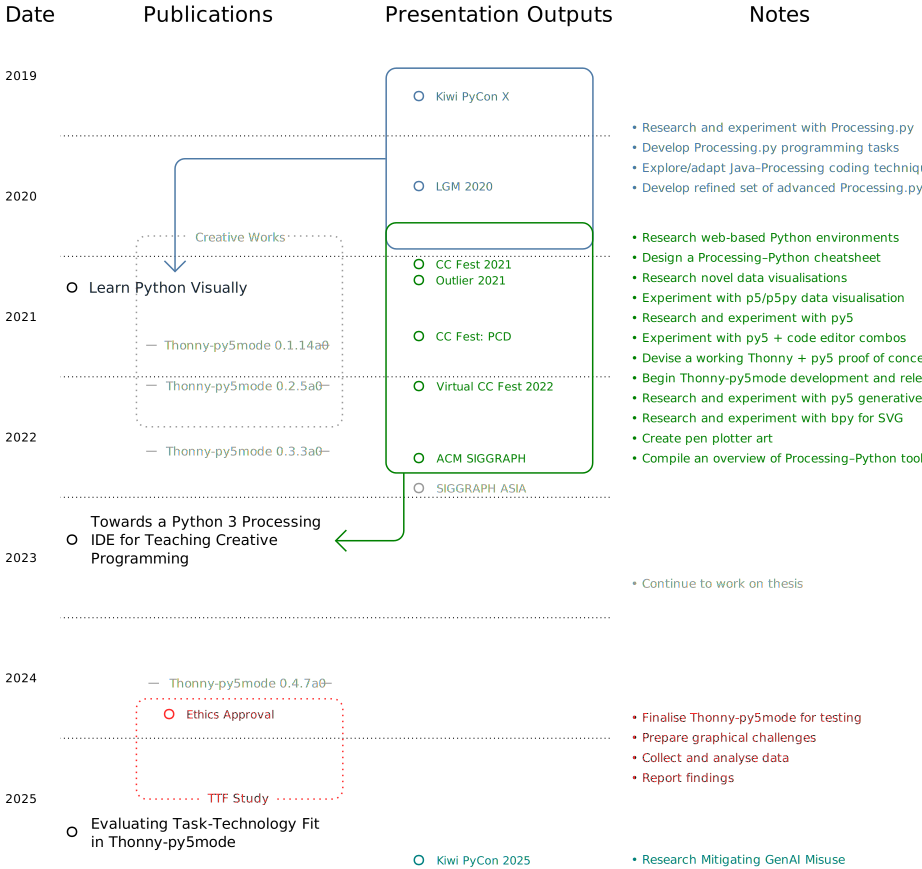
\includegraphics[width=1.0\textwidth]{chapters/chapter04-publications/publications-chart}
\smallskip
\caption{Timeline of publications, highlighting the integration of presentation outputs (talks, workshops, and demonstrations) into the research process. Diagram by the author.}
\label{fig:publications-chart}
\end{figure}

The \textit{Publications} column lists the three works discussed in this chapter, shown in \textbf{bold black type}. Within this column, several \textcolor{gray}{\textit{--- Thonny-py5mode...}} entries indicate individual Thonny-py5mode releases. Dotted-outline cells mark the periods of producing the \textit{Creative Works} (covered in the \nameref{chap:creative-works} chapter) and conducting the empirical evaluation of Thonny-py5mode (\textit{TTF Study}). The \textit{Notes} column summarises the processes and steps that defined each stage.

Viewed within the context of this PhD by folio/publication, the sole-authored book and two peer reviewed Q1/Q2 journal articles balance practical impact with scholarly rigour. \textit{\nameref{sec:no-starch}} serves as a resource for educators integrating Python-based creative coding into curricula, while the journal articles contribute to academic discussion surrounding Python tools for visual learning contexts. Collectively, these publications address four research objectives outlined in the ``\nameref*{chap:introduction}'' chapter: \hyperref[ro:tool-development]{Tool Development}, \hyperref[ro:educational-materials]{Educational Materials}, \hyperref[ro:empirical-evaluation]{Empirical Evaluation}, and \hyperref[ro:broader-dissemination]{Broader Dissemination}.

As outlined in Figure~\ref{fig:literature-review-conceptual-map} in the ``\nameref*{chap:literature-review}'' chapter, the journal articles engage with much of the relevant literature, as do the \nameref{chap:presentation-outputs} and, to a lesser extent, the \nameref{chap:creative-works}. Given the folio/publication thesis format, some of the literature in the journal articles unavoidably overlaps with the \nameref*{chap:literature-review}. Specifically---

\begin{itemize}

\item While the ``\nameref*{chap:literature-review}'' chapter also covers prominent creative coding environments, the article \textit{\nameref{sec:mtap}} extends this analysis to explore Python-3-specific creative coding environments in greater depth.

\item The other article, \textit{\nameref{sec:jise}}, reiterates some of the general and introductory literature on creative coding environments in a more condensed form. However, it also provides an additional review of scholarship supporting the Task--Technology Fit framework, which is central to its study.

\end{itemize}

The next section (\ref{sec:no-starch}) reviews the content and development of the book \textit{\nameref{sec:no-starch}}, which cannot be reproduced in full here because of its length and copyright restrictions. Following that, the subsequent sections (\ref{sec:mtap}, \ref{sec:jise}) present the two journal articles in their preprint (submitted) form, which do not incorporate revisions made after peer review. Publishers permit the distribution and archiving of these versions, which exclude publisher formatting and instead follow the style and conventions of the thesis.

%%%%%%%%%%%%%%%%%%%%%%%%%%%%%%%%%%%%%%%%%%%%%%%%%%%%%%%%%%%%%%%%%%%%%%%%%%%%%%%
%%%%%%%%%%%%%%%%%%%%%%%%%%%%%%%%%%%%%%%%%%%%%%%%%%%%%%%%%%%%%%%%%%%%%%%%%%%%%%%

\cleardoublepage
\section{Learn Python Visually: Creative Coding with Processing.py}
\label{sec:no-starch}
\vspace{1.5em}
\begin{outputmeta}
\textbf{Publisher}: No Starch Press \\
\textbf{Publisher URL}: \url{https://nostarch.com} \\
\textbf{Author(s)}: Bunn, T. \\
\textbf{Date published}: 20 July 2021 \\
\textbf{ISBN-13}: 978-1-7185-0096-9 \\
\textbf{Print length}:‎ 296 pages \\
\textbf{Catalogue entry}: \url{https://nostarch.com/Learn-Python-Visually} \\
\textbf{Publication evidence}: See Appendix \ref{appendix:no-starch-cover}
\end{outputmeta}
\subsection{Background \& Context}

\textit{Learn Python Visually} (Figure~\ref{fig:book-cover-photo}) represented a significant component of this PhD research, concluding the initial phase of investigation into- and development of novel Python-based creative coding techniques. Aimed at beginner coders and readers transitioning from other programming backgrounds, the book employs Processing's Python Mode (Processing.py) as its pedagogical foundation, combining Python's accessibility with Processing's multimedia capabilities.

\begin{figure}[htbp]
\centering
\includegraphics[width=1\textwidth]{chapters/chapter04-publications/no-starch/book-cover-photo}
\caption{\textit{Learn Python Visually: Creative Coding with Processing.py}. Photo by the author.}
\label{fig:book-cover-photo}
\end{figure}

The book's strength and novelty lie in its visual and practical take on Python instruction. Each chapter builds progressively upon the last, moving from fundamental concepts toward more sophisticated creative coding techniques. This approach directly aligns with the overarching aim of the thesis: enhancing Python programming education through creative computing environments, and specifically the \hyperref[ro:educational-materials]{Educational Materials} and \hyperref[ro:broader-dissemination]{Broader Dissemination} objectives. Two presentations in particular, \nameref{sec:processing.py-creative-coding-with-python} and \nameref{sec:processing-python-mode-for-creative-coding-and-teaching}, provide further insight into the activities and research that informed the book's development. 

No Starch Press is a respected independent publisher specialising in technical and educational titles. Established in 1994, it has built a strong reputation for publishing accessible yet rigorous works on programming, cybersecurity, and STEM education, including bestsellers such as \textit{Python Crash Course}, \textit{Python for Kids}, \textit{How Linux Works}, and \textit{Hacking: The Art of Exploitation}. Its titles---widely adopted by learners, educators, and professionals---have received industry recognition, including Independent Publisher Book Awards (from \textit{Independent Publisher} magazine) and inclusion in the prestigious \textit{Communication Arts Design Annual}. This status underscores the book's credibility as both a practical learning resource and a contribution to Python-based programming education~\cite{no_starch_press_about_2025}.

Paddy Gaunt, who served as the book's technical reviewer, studied engineering at Cambridge University (UK). Since 2012, he has maintained pi3d: a Python library designed to deliver high-speed 3D graphics on Raspberry Pi microcomputers~\cite{bunn_learn_2021}.

\textit{Learn Python Visually} is available worldwide in both print and digital formats. It has received favourable reviews on Amazon.com\footnote{~\url{https://www.amazon.com/Learn-Python-Visually-Tristan-Bunn/dp/1718500963}} where it features editorial endorsements from Saber Khan (Education Community Director of the Processing Foundation), Dr.~Ralf Biedert (Principal Engineer at Tobii AB), and Alfred Abusomwan (Techs Blog). As of June 2025, the book had achieved 2,622 direct sales (Appendix \ref{appendix:no-starch-royalty-statement}). It was also included in two Humble Bundle collections: \textit{Machine Learning by No Starch Press} (August 2021) and \textit{Python by No Starch Press} (May 2023), that sold 17,669 and 10,881 bundles, respectively~\cite{humble_bundle_inc_machine_2021, humble_bundle_inc_humble_2023}. 

In addition to direct and bundled sales, the book is distributed internationally through No Starch Press partners, including digital platforms such as O'Reilly Online Learning\footnote{~\url{https://www.oreilly.com/library/view/learn-python-visually/9781098128937}} and through academic library collections, further extending its educational reach. Penguin Random House distributes No Starch Press printed titles in the USA and worldwide~\cite{no_starch_press_sales_2025}.

\textit{Learn Python Visually} integrates visual learning throughout its chapters, requiring learners to program output that expresses computational methods through graphical outputs, animations, data visualisations, 2D simulations, and interactive interfaces. In this way, it places emphasis on immediate, observable results to elucidate abstract concepts and support intuitive understanding. The book is printed in full colour, incorporating visual explanations in addition to the results of different code samples. Figures~\ref{fig:book-p190-p205} and~\ref{fig:book-p210-p225} present a sample selection of 16 pages each.

\begin{figure}[htbp]
\centering
\includegraphics[width=\textwidth]{chapters/chapter04-publications/no-starch/book-p190-p205}
\caption{Excerpt from the author's book \textit{Learn Python Visually} (pp.~190--205), published by No Starch Press. This section introduces trigonometric functions and waveforms, and demonstrates the generation of Lissajous figures using Python. Source:~\cite{bunn_learn_2021}.}
\label{fig:book-p190-p205}
\end{figure}

\begin{figure}[htbp]
\centering
\includegraphics[width=\textwidth]{chapters/chapter04-publications/no-starch/book-p210-p225}
\caption{Excerpt from the author's book \textit{Learn Python Visually} (pp.~210--225), published by No Starch Press. This section introduces object-oriented principles through the generation of an amoeba simulation using Python. Source:~\cite{bunn_learn_2021}.}
\label{fig:book-p210-p225}
\end{figure}

The early chapters cover introductory concepts, such as installation procedures, basic syntax, arithmetic operations, and the principles of drawing with code. Once readers are familiar with the fundamentals, later chapters build on these foundations, shifting focus to concepts that require more programmatic reasoning---control flow, iteration, randomness, motion, transformations, data visualisation, and constructing a user interface. The following outline provides a brief overview of each chapter's contents:

\begin{quote}

\noindent\textbf{Chapter 1: Hello, World!} \\
Covers installation and setup for Processing Python Mode (Processing.py) and introduces the basics of drawing with code. Also: how computers manage colour, how to store and reuse values using variables, and how to perform basic arithmetic operations in Python.

\vspace{0.5em}
\noindent\textbf{Chapter 2: Drawing More Complicated Shapes} \\
Building on drawing essentials, readers move on to organic (non-geometric) shapes---defining these with points (vertices) and curves, which can describe almost any 2D form in code.

\vspace{0.5em}
\noindent\textbf{Chapter 3: Introduction to Strings and Working with Text} \\
Introduces Python's string features for manipulating text. To visualise these concepts, readers explore Processing functions for drawing text to the display window in different styles, colours, and fonts.

\vspace{0.5em}
\noindent\textbf{Chapter 4: Conditional Statements} \\
Moving into control flow, demonstrating how to write programs that make decisions and execute different actions in response to different situations. Again, readers explore these concepts through graphical output.

\vspace{0.5em}
\noindent\textbf{Chapter 5: Iteration and Randomness} \\
Covers repeating operations in Python, either a specified number of times or until a condition is met. Readers combine these techniques with randomness to generate tiled patterns.

\vspace{0.5em}
\noindent\textbf{Chapter 6: Motion and Transformation} \\
Introduces the \texttt{draw()} function for animated output. Also covers saving frames as images, transforming groups of visual elements, and employing real-time values for screensavers and clock displays.

\vspace{0.5em}
\noindent\textbf{Chapter 7: Working with Lists and Reading Data} \\
Unlocks techniques for managing and manipulating collections of values, leading to practical data visualisation examples that read in external CSV data to generate charts dynamically.

\vspace{0.5em}
\noindent\textbf{Chapter 8: Dictionaries and JSON} \\
Explores richer data structures and visualisation with JSON data, developing readers' skills to work with more complex and novel data visualisations.

\vspace{0.5em}
\noindent\textbf{Chapter 9: Functions and Periodic Motion} \\
Shows how dividing programs into reusable functions improves modularity and readability, then combines these techniques with trigonometric operations to generate elliptical and wave-type motions.

\vspace{0.5em}
\noindent\textbf{Chapter 10: Object-Oriented Programming and PVector} \\
Demonstrates object-oriented principles to structure programs that model real-world phenomena, guiding readers through programming a visually engaging amoeba simulation that leverages vector-based motion.

\vspace{0.5em}
\noindent\textbf{Chapter 11: Mouse and Keyboard Interaction} \\
Concludes the book by adding interactivity to Processing sketches, focusing on mouse and keyboard input to build a paint app. This requires event functions and techniques for controlling Processing's draw-loop behaviour.

\end{quote}

An Afterword discusses where readers might head next, pointing them to the Processing community forum and useful materials, including tutorials on working with Images \& Pixels, P3D for 3D work, and the broader Processing ecosystem of libraries (written for Java Mode but typically portable to Python Mode). It encourages translating Java examples, highlights Daniel Shiffman's \textit{The Nature of Code} (with Python ports), and discusses Python's applications in games, the web, data, and AI. Additionally, there is some discussion on adjacent creative-coding environments, including p5.js, JRubyArt, openFrameworks, OPENRNDR, and hardware programming with Arduino.

Notably, readers' prior experience in related areas, including other programming languages, will likely influence their comprehension and the pace at which they progress through the book. However, the text encourages detours wherever inspiration strikes and includes challenges and practical tasks at key moments to reinforce conceptual understanding and promote active learning. For complete beginners, the content aims to reduce the anxiety often associated with textual coding by incorporating visual tasks wherever possible.

\subsection{Conclusion}

Within the framework of this thesis, \textit{Learn Python Visually} consolidates extensive research into Python creative computing, specifically the Processing.py environment, translating experimental work into pedagogical strategies and learning materials. Publication by No Starch Press (est.~1994), with technical review by Paddy Gaunt (maintainer of pi3d), attests to rigour. Uptake indicators include 2,492 direct sales as of Dec~2024, inclusion in two Humble Bundle collections that together sold more than 25,000 digital copies, and worldwide distribution. Collectively, these figures evidence effective pedagogy and and broad accessibility.


%%%%%%%%%%%%%%%%%%%%%%%%%%%%%%%%%%%%%%%%%%%%%%%%%%%%%%%%%%%%%%%%%%%%%%%%%%%%%%%
%%%%%%%%%%%%%%%%%%%%%%%%%%%%%%%%%%%%%%%%%%%%%%%%%%%%%%%%%%%%%%%%%%%%%%%%%%%%%%%

\cleardoublepage
\section{Towards a Python 3 Processing IDE for Teaching Creative Programming}
\label{sec:mtap}
\vspace{1.5em}
\begin{outputmeta}
\textbf{Journal}: Multimedia Tools and Applications \\
\textbf{Journal Ranking}: Q1 (see \href{https://www.scimagojr.com/journalsearch.php?q=25627&tip=sid}{Scimago Journal \& Country Rank}) \\
\textbf{Author(s)}: Bunn, T., Anslow, C., and Lundqvist, K. \\
\textbf{Statement of Authorship}: See Appendix \ref{appendix:statement-of-authorship-mtap} \\
\textbf{Date Received}: 06 March 2023 \\
\textbf{Date Published}: 10 October 2024 \\
\textbf{DOI}: \url{https://doi.org/10.1007/s11042-024-20345-1} \\
\textbf{Publication Evidence}: See Appendix \ref{appendix:mtap-website}
\end{outputmeta}
\subsection{Abstract}

\textit{Processing} is a popular graphical library and IDE developed for electronic art and visual design communities, with a strong focus on teaching art, design, and creative technologies students computer programming fundamentals in a visual context. Processing provides a collection of special commands to draw, animate, and handle user input using Java. Users can enable Python Mode (also called Processing.py) for Processing in the IDE interface. This leverages Jython, a Java implementation of Python, to interface with Processing's Java core, providing a way to write Processing code using Python syntax. 

This paper proposes that combining Processing and Python provides an ideal development environment for teaching creative programming fundamentals. Several new Processing-Python environments and tools have emerged, but no attempts to integrate one of the most promising, the \textit{py5} library created by Jim Schmitz, into a Processing-like-IDE experience. py5 offers features not available with Jython, such as compatibility with Python 3 and support for CPython libraries. This paper presents a new coding environment, Thonny-py5mode, developed as a software plugin for the Thonny IDE, which brings a convenient, beginner-friendly setup like that of Processing's Python Mode to users working with py5.

\bigskip

\noindent\textit{\textbf{CCS Concepts: Applied computing \texttt{→} Media arts; Interactive learning environments; Education.}} \textit{Additional Key Words and Phrases: Processing, py5, Python Mode, Processing.py, Python}

\begin{figure}[htbp]
\includegraphics[width=\textwidth]{chapters/chapter04-publications/mtap/figure-teaser}
\caption{Running a py5 sketch using Thonny-py5mode. Screenshot by the author.}
\label{fig:teaser}
\end{figure}

\subsection{Introduction}

Processing is an open-source integrated development environment (IDE) popular for teaching non-programmers the fundamentals of computer programming in a visual context. Since 2001, Processing has promoted software literacy within the visual arts and visual literacy within technology. Tens of thousands of students, artists, designers, researchers, and hobbyists use Processing and its related projects\footnote{~\url{https://processing.org}} for learning, prototyping, and a diverse range of creative computing projects~\cite{noble_programming_2009}. 

Alternative Processing programming libraries include p5.js (for JavaScript), JRubyArt (for Ruby), and even an effort to create a version for the R language~\cite{wikipedia_processing_2025}. Python Mode for Processing---which some people refer to as Processing.py---combines the Python programming language and Processing~\cite{parrish_getting_2016}, providing users with a Python alternative to Processing's Java syntax. Figure~\ref{fig:figure-processing-py-vs-processing-java} contrasts Processing's Java and Python modes, demonstrating how programmers interface with the same API, using the same IDE, with different syntax. In this instance, the resulting output is an animated square that moves from the left to the right of the display window (leaving a trail of visible frames in its wake).

\begin{figure}[htbp]
\includegraphics[width=\textwidth]{chapters/chapter04-publications/mtap/figure-processing-py-vs-processing-java}
\caption{Processing in its original Java mode (left) and Python mode (right). Screenshots by the author.}
\label{fig:figure-processing-py-vs-processing-java}
\end{figure}

\subsubsection{Java and Python for Introductory Programming Lessons}

Interestingly, reports from the IEEE (Institute of Electrical and Electronics Engineers) indicate that both Java and Python have been among the top-ten-list of programming languages in recent years~\cite{cass_top_2022}. While Processing-Java's success suggests it is a highly effective way to learn to program, the Java syntax may be less ideal than Python syntax---as this paper argues, particularly for visual design and art students. 

There has been an ongoing debate about which language is best for novices and teaching programming~\cite{pears_survey_2007}. Studies highlight Python's strong and growing presence in introductory Computer Science curricula~\cite{guo_python_2014}, courses for other domains that employ programming~\cite{duda_teaching_2021, ling_can_2021, riedl_python_2015}, and other educational environments~\cite{tabet_alice_2016}. Python overtook Java as the most popular introductory teaching language at top U.S. Universities in 2014~\cite{guo_python_2014}. To return to Figure~\ref{fig:figure-processing-py-vs-processing-java}, Python offers a more shallow abstraction gradient. It does not require semi-colons to terminate each line and drops the braces in favour of prescribed indentation. An educator does not need to explain to students what Java's \texttt{void} does, which involves understanding how functions return data, something not typically covered in the first lesson of a novice programming course. Learning to code with Processing and Python also provides an entry to other domains of Python programming, including artificial intelligence, data-science and visualisation, game development, web development, desktop applications, and web scraping. Python includes many characteristic features for supporting learning (by abstracting away some more complex concepts), including small and clean syntax, dynamic typing, expressive semantics, immediate feedback, and object orientation~\cite{grandell_why_2006}.

\subsubsection{Potential Advantages of Processing-Python over Processing-Java}

Educators can leverage the advantages of Python described in the previous subsection by employing Python to write Processing code. 

In 2008, Bälter and Dale~\cite{balter_enjoying_2010} experimented with an introductory programming course that combined Python, Processing, and Core Java. They opted to introduce coding fundamentals for the first four weeks using Python, shifted to two weeks of Processing-Java following that for its graphics capabilities, and then concluded with a final four weeks of Processing and Java followed by a four-week student-determined final project. The vast majority, 16 of the 26 students, chose Processing for their final projects, while four used text-based Java. In their conclusion, Bälter and Dale mention Nodebox (a Python-based Mac OS X Processing alternative) as an all-Python option for similar courses, which was still under development at the time. A few years later, Processing's Python Mode would combine all those technologies (Python, Processing, and Core Java) into a single IDE, effectively enabling such a course to employ Python throughout. 

In 2013, Frederik Berlaen would redesign DrawBot for macOS, a Processing-inspired environment for creating two-dimensional graphics using Python code. DrawBot has proven itself as part of the curriculum within selected courses at the Royal Academy of Art in The Hague.\footnote{~\url{https://www.drawbot.com/\#education}} Several other Processing-like Python options have since appeared, reviewed in Section \ref{Tools Combining Processing and Python}. This proliferation of Python-based Processing-like environments, many led by people involved in education, points to an identified desire for teaching using Python creative coding environments. 

The Python language should help novices writing Processing code to produce results (visual output in this case) more rapidly, heightening their sense of accomplishment. As Hsiao-Chi \textit{et al.} conclude in their multi-group study of students learning programming~\cite{ling_can_2021}, compared with students who learn Java, Python students are more likely to: reduce their maladaptive cognition; improve their self-efficacy and motivation to learn; feel a greater sense of learning achievement. Processing-Python solutions, therefore, provide an arguably more beginner-friendly and approachable (Python-based) experience than Processing-Java and, at the same time, offer many/all the same graphics and multimedia programming features~\cite{bunn_learn_2021}.

After the release of Processing version 4 in August 2020, Ben Fry, co-creator of Processing, wrote on the potential of porting the entire project to Python\footnote{~\url{https://github.com/benfry/processing4/wiki/Processing-4}}, citing issues with Java, particularly Oracle's handling of the product. Fry labelled Python as ``terrific,'' although lacking readily available components for interactive graphics, and described the Python Mode (Jython) implementation as ``great''. However, he desired the ``NumPy [library] and all those other things that make Python wonderful''---a shortcoming addressed in py5. As the official py5 documentation describes~\cite{schmitz_welcome_2021}:

\medskip

\noindent\textit{``Processing.py [see Processing Python Mode] is the spiritual ancestor to and inspiration for py5. [It] is similar to Processing.py in that both use Python syntax but their implementations are very different. Processing.py and py5 do not share any code but py5 benefits from code in the Processing core libraries written to accommodate Processing.py.''}

\medskip

Compared with Processing, py5 also includes Python-style naming conventions, various Processing enhancements for named and shorthand hexadecimal colour values, NumPy methods for selecting and manipulating pixels, profiler functions, and OpenSimplex 2 noise. 

\subsubsection{Processing Python Mode / Processing.py Limitations}

Figure~\ref{fig:figure-processing-py-workings} illustrates at a very high level how Processing Python Mode passes code from the editor to Jython so that Java may interpret it. However, Processing.py's Jython implementation has its limitations: (a) it is source-compatible with Python 2.7 (not 3+), which the Python Software foundation officially sunset\footnote{~\url{https://www.python.org/doc/sunset-python-2}} on January 1, 2020; (b) it does not support CPython libraries, such as NumPy for handling complex matrix operations or Pymunk for simulating 2D physics. 

\begin{figure}[htbp]
\includegraphics[width=\linewidth]{chapters/chapter04-publications/mtap/figure-processing-py-workings}
\caption{Processing Python Mode's Jython implementation. Diagram by the author.}
\label{fig:figure-processing-py-workings}
\end{figure}

This paper presents a new Processing-inspired development environment, Thonny-py5mode, which supports Python 3 and CPython libraries (via py5) that the author (Bunn) developed as a software plugin for the Thonny IDE.

\subsection{The Thonny-py5mode Plugin}
\label{sec:the-thonny-py5mode-plugin}

Thonny is a beginner-oriented IDE for Python programming, including an embedded CPython (3.x) interpreter, features for explaining variable scope, and a GUI for managing Python packages. The Thonny-py5mode plugin installs JRE and configures Thonny for use with py5. It adds assistive Processing-like features to the Thonny editor, including syntax-highlighting and hinting for py5 functions and keywords, a colour mixer, menu items for converting code between Processing.py and py5, a py5 quick reference, and a Processing-IDE-inspired colour scheme. It provides a much-needed successor to the Processing IDE's Python Mode coding experience, transforming Thonny into a creative computing environment by adding features that employ Processing's core libraries to generate interactive visual output via py5.

py5 provides module, class, imported, and static modes, and the Thonny-py5mode plugin can switch how it runs code to support the mode the user wishes to employ. For example, static mode is the simplest way to start writing code as it does not require any \texttt{import} lines or even \texttt{setup()} and \texttt{draw()} blocks. In static mode, drawing a square requires nothing more than a single line with a \texttt{square()} function (and the appropriate three arguments for x-coordinate, y-coordinate, and extent). 

The py5 and Thonny-py5mode communities are overlapping groups of people, and ongoing discussion between those developers and users informs new features for both projects. On the other hand, work on the Processing Python Mode / Processing.py project has largely stalled, and the project has sought (unsuccessfully) a new leader for some time~\cite{feinburg_python_2023}. 

The Thonny-py5mode plugin removes the complexity beginner programmers may face setting up a working py5 environment (installing Python, setting up a Java Runtime Environment, configuring a suitable code editor, and so on). Effectively, it emulates the successful approach adopted in Processing's Python Mode. Namely, a simple-to-activate mode for an existing IDE that conveniently transforms it into a Python environment for creative computing. Thonny-py5mode makes it easy for beginners to start with py5, also serving as an immediately familiar alternative for anybody familiar with the Processing IDE (especially its Python Mode).

Figure~\ref{fig:figure-thonny-py5mode-workings} depicts the Thonny interface with the plugin installed as part of a diagram that approximately contrasts the workings of py5 (which employs JPype over Jython) against those of Processing's Python Mode (Figure~\ref{fig:figure-processing-py-workings}). Note that the code editors may look the same or similar because the Thonny IDE has its Processing-style theme active that Thonny-py5mode applies.

\begin{figure}[htbp]
  \centering
  \includegraphics[width=\linewidth]{chapters/chapter04-publications/mtap/figure-thonny-py5mode-workings}
  \caption{The Thonny IDE with Thonny-py5mode activated. py5 uses JPype to interface between Python 3 and Processing's Java libraries. Diagram by the author.}
  \label{fig:figure-thonny-py5mode-workings}
\end{figure}

The Thonny IDE includes a graphic interface for managing Python packages (Figure~\ref{fig:figure-pymunk}) to make it easy for users to install additional packages such as Pymunk for incorporating 2D physics in simulations programmed with py5. This interface avoids users having to use a command-line interface for managing Python packages.

\begin{figure}[htbp]
  \centering
  \includegraphics[width=\linewidth]{chapters/chapter04-publications/mtap/figure-pymunk}
  \caption{Installing Pymunk via the Thonny package manager. Screenshot by the author.}
  \label{fig:figure-pymunk}
\end{figure}

\subsection{Tools Combining Processing and Python} \label{Tools Combining Processing and Python}

The introduction section mentions that several new Processing-Python environments and tools have emerged as Python Mode alternatives. This section reviews those, providing technical insight into their differences, and discussing the advantages and disadvantages of each approach. It also reiterates and highlights the benefits that Thonny-py5mode provides as a new Python-based creative programming environment for teachers, learners or beginners, and creative coders.

In a systematic review of different Python-based programming options for design and architectural education, Villares and de Carvalho Moreira~\cite{villares_python_2017} survey 43 environments/tools, ``of which 32 at least [are] superficially investigated, [and] at least 20\% (7 of 32) have substantial educational aims.'' The study highlights Python's strong and growing presence in introductory computer science curricula, creative computing courses, and other educational settings. Python is well-suited to novice programmers, and Processing provides a proven environment for teaching textual programming, especially to art, design, and other `visually-oriented' students~\cite{greenberg_processing_2016, reas_processing_2006, reas_processing_2014}. Processing Python Mode may, therefore, seem like an ideal for teaching creative programming, but its Jython component has limitations. 

\subsubsection{Web-Browser-Based Options}

Villares provides a table (Table \ref{tbl:table-processing+python}) of different Processing + Python software that has emerged in recent years. The bottom four entries in Table \ref{tbl:table-processing+python} are web-browser-based. Three of those, pyp5js (depicted in Figure~\ref{fig:figure-pyp5js}), Proceso, and BrythonIDE, combine p5.js (JavaScript) and Python using Pyodide, Transcrypt, or Brython; the other web-browser-based approach, employed in SkulptIDE and trinket.io, utilises ProcessingJS (JavaScript), but development on ProcessingJS ceased a while before 2018.\footnote{~\url{https://github.com/processing-js/processing-js}}

\begin{table}[!htbp]
  \centering
  \rotatebox{90}{
    \begin{minipage}{0.96\textheight}
      \centering
      \fontsize{9.7pt}{11pt}\selectfont{}
      \renewcommand{\arraystretch}{1.5}
      \begin{tabular}{
        >{\raggedright\arraybackslash}p{\dimexpr 0.14\linewidth-2\tabcolsep}
        >{\raggedright\arraybackslash}p{\dimexpr 0.14\linewidth-2\tabcolsep}
        >{\raggedright\arraybackslash}p{\dimexpr 0.11\linewidth-2\tabcolsep}
        >{\raggedright\arraybackslash}p{\dimexpr 0.11\linewidth-2\tabcolsep}
        >{\raggedright\arraybackslash}p{\dimexpr 0.11\linewidth-2\tabcolsep}
        >{\raggedright\arraybackslash}p{\dimexpr 0.195\linewidth-2\tabcolsep}
        >{\raggedright\arraybackslash}p{\dimexpr 0.195\linewidth-2\tabcolsep}
      }
        \hline
        \textbf{Name} & \textbf{Processing features} & \textbf{Based on (and Python ver.)} & \textbf{Python std. library} & \textbf{Libraries ecosystem} & \textbf{Main features} & \textbf{Main limitations} \\
        \hline
        Processing Python Mode (the "reference implementation" for comparison) &
        Processing 3 Java &
        Jython (Python 2) &
        Complete &
        Java and Processing Java &
        Available inside Processing IDE; highly Processing-3-compatible &
        Processing 4 incompatible; no web sharing; no modern Python 3 libs; needs new maintainer \\
        \hline
        py5 &
        Processing Java graphics via JPype &
        Python 3 &
        Complete &
        Python and Processing Java &
        Truly Python-3-compatible library support; Jupyter notebooks support; core capabilities of Processing 4 Java &
        Snake\_case names; experimental; some Processing Java libraries may not work \\
        \hline
        p5py &
        New implementation based on OpenGL (incomplete), and will add Skia back-end &
        Python 3 &
        Complete &
        Python only &
        Truly Python-compatible; no Java/JVM dependency &
        Snake\_case names; experimental; still incomplete; no access to Processing Java libraries \\
        \hline
        pyp5js (Pyodide or Transcrypt mode) &
        p5.js &
        Python 3 via Pyodide or Transcrypt &
        Complete &
        Python, JavaScript and p5.js &
        Web-ready sketches and editor; highly p5.js-compatible; Pyodide is highly Python-compatible &
        Experimental; still incomplete; p5.js features (as opposed to Processing Java/Python modes) \\
        \hline
        Proceso &
        p5.js &
        Python 3 via Pyodide &
        Complete &
        Python, JavaScript and p5.js &
        Browser-based sketches; highly p5.js compatible; Python-compatible; names similar to py5 &
        p5.js features (as opposed to Processing Java/Python modes) \\
        \hline
        SkulptIDE and trinket.io &
        ProcessingJS &
        Skulpt (Python 2, but migrating to 3) &
        Partial &
        Unknown, possibly JavaScript &
        Appealing and refined web IDE; browser-based sketches &
        ProcessingJS is defunct; not extensible \\
        \hline
        BrythonIDE and p5py.com &
        p5.js &
        Brython (Python 3) &
        Fairly complete &
        JavaScript and p5.js &
        Browser IDE; browser-based sketches; highly p5.js-compatible &
        p5.js features (as opposed to Processing Java/Python modes) \\
        \hline
      \end{tabular}
      \caption{Processing + Python tools table. Adapted from Villares~\cite{villares_resources_2022}.}
      \label{tbl:table-processing+python}
    \end{minipage}
  }
\end{table}

\begin{figure}[htbp]
  \centering
  \includegraphics[width=0.8\linewidth]{chapters/chapter04-publications/mtap/figure-pyp5js}
  \captionsetup{width=0.8\textwidth}
  \caption{Running a p5.js--Python sketch in a web browser using pyp5js. Screenshot by the author.}
  \label{fig:figure-pyp5js}
\end{figure}

Browser-based solutions have the advantage of running on any platform with a modern web browser. These solutions offer the quickest means to start writing and executing code and are helpful in many situations where downloading additional software can be problematic. However, these cannot utilise the rich ecosystem of Processing-Java libraries because none interface with Java in any way. While the p5.js project offers a robust collection of libraries, other Python libraries from the Python Package Index (PyPI) may be unavailable or could prove challenging for beginners to set up.\footnote{~Refer to Brython, Pyodide, and Transcrypt official documentation for package availability and limitations} 

py5 also supports a browser-based coding environment through Jupyter Notebooks, an open-source web application popular among scientists and researchers~\cite{granger_jupyter_2021}. While web-browser-based solutions are preferable in several situations, and Jupyter Notebooks brings a host of valuable features, this paper focuses on a Python 3 alternative for a Processing-Java \textbf{desktop} IDE.

\subsubsection{Comparing Thonny-py5mode and Processing (and similar) Desktop IDEs}

Villares' table \ref{tbl:table-processing+python} lists a single solution (Processing Python Mode) using a desktop (opposed to browser-based) IDE. With some relatively simple to involved configuration effort, users can employ a general-purpose desktop IDE (such as Visual Studio Code, Geany, or similar) for Processing, py5, p5py, or pyp5js. However, Thonny-py5mode aims to provide a multi-platform desktop IDE experience for beginners with little to no configuration required. Moreover, it includes many features specific to py5 that a user could not access in a more general-purpose IDE. 

Drawbot, Nodebox, and Shoebot are pure Python alternatives to the Processing IDE absent from Villares' table of different Processing + Python environments/tools. None leverage the Processing API. Drawbot and Nodebox provide ready-configured/bespoke desktop IDEs, but those support Apple Mac platforms exclusively. Shoebot is a multi-platform port/rewrite of Nodebox, which also features a bespoke IDE~. Shoebot does not provide the extensive features of the Thonny-py5mode plugin, including syntax highlighting and hinting for functions and keywords, a colour mixer, menu items for converting code from Processing.py scripts, and a package manager for installing other Python packages. The Shoebot installation process is also more involved, requiring users to install several dependencies. Shoebot started in 2007 and transitioned from Python version 2 to 3; it is a capable coding environment, particularly for vector graphics, and remains an interesting open-source project to watch.

The p5py project (Figure~\ref{fig:figure-p5py}) has made good progress on developing a native Python 3 port of the Processing API. However, a few core individuals currently driving the p5py project must effectively recreate the entire Processing API from scratch in Python. py5, instead, leverages the mature Processing-Java codebase via JPype, actively developed by a large community of programmers. p5py has no desktop IDE plugin like Thonny-py5mode, or Jupyter Notebooks kernels, and users must install GLFW (a multi-platform OpenGL library) separately. However, p5py is useful for anybody seeking a pure-Python library to programme simulations and interactive art, accumulating 700 stars\footnote{~\url{https://github.com/p5py/p5}} on GitHub to date.

\begin{figure}[htbp]
  \centering
  \includegraphics[width=0.8\linewidth]{chapters/chapter04-publications/mtap/figure-p5py}
  \captionsetup{width=0.8\textwidth}
  \caption{Writing p5py code in a general-purpose code editor (not a bespoke IDE or plugin). Screenshot by the author.}
  \label{fig:figure-p5py}
\end{figure}

Neither py5 nor p5py provides a Processing kind of IDE experience. That is, a bundled code editor with features specifically to complement working with their libraries. Hence, the opportunity to create a Processing Python Mode / Processing.py successor by way of a Thonny IDE plugin.

\subsection{thonny-py5-mode Examples}

Accomplished creative coders and beginners alike have employed the Thonny-py5mode environment for programming generative artworks. Figure~\ref{fig:figure-aquatics} presents an adaptation of Lieven Menschaert's NodeBox script, Aquatics, programmed using Thonny-py5mode. This spawns a creature with a random fill colour, shape (defined by something named the superformula), and no fewer than three eyes. There is a 70 percent chance that hair will grow along the creature's edges, which can be swayed by the force of a randomly directed current.

\begin{figure}[htbp]
  \centering
  \includegraphics[width=\linewidth]{chapters/chapter04-publications/mtap/figure-aquatics}
  \caption{Artwork inspired by Lieven Menschaert's NodeBox script \textit{Aquatics}, programmed using Thonny-py5mode. Artwork by the author.}
  \label{fig:figure-aquatics}
\end{figure}

2-Axis pen plotters provide another fun way for students or artists to experiment with generative output using ink and paper. Again, the Thonny package manager makes it convenient to install the powerful Python library, vpype---a ``Swiss-Army-knife'' for working with vector graphics for plotters~\cite{beyeler_vpype_2022}. Using vpype, the programmer can perform some post-processing on py5-generated SVG files to optimise paths for pen plotting. Figure~\ref{fig:figure-plot} shows a Thonny-py5mode program that generates SVG files that the creator will plot using different colour pens.

\begin{figure}[htbp]
  \centering
  \includegraphics[width=\linewidth]{chapters/chapter04-publications/mtap/figure-plot}
  \caption{Programming generative (multi-pen) plotter art in the Thonny-py5mode environment. Screenshot by the author.}
  \label{fig:figure-plot}
\end{figure}

A wide variety of other projects might employ Thonny-py5mode, including for visual art and design work, video games, installation artworks and projections, sound art, prototypes, and other creative applications. Reviewing different results created using Processing, OpenFrameworks, and OPENRNDR offers inspiration for what is possible. 

\subsection{Thonny-py5mode in the Classroom}

At Massey University's College of Creative Arts in New Zealand, educators adapted a course that used Processing's Python Mode to one using Thonny-py5mode for 2022. This required revising the course learning materials, which also served as part of the py5 project's efforts to develop tutorial documentation. The Processing Foundation co-funded Zelle Marcovicci for the documentation work, mentored by Jim Schmitz and Tristan Bunn. Materials went `live' on the official \href{https://py5coding.org}{py5coding.org} website later in 2022~\cite{processing_foundation_google_2022}. To date, there is no comparative study to assess the 2022 cohort's experience and abilities against those of the previous cohorts who used Processing's Python Mode. Figure~\ref{fig:figure-penno-avatars} is an example of one student's submission at the mid-point of the course, after roughly 5 × 2-hour training workshops using Thonny-py5mode. 

\begin{figure}[htbp]
  \centering
  \includegraphics[width=\linewidth]{chapters/chapter04-publications/mtap/figure-penno-avatars}
  \caption{Abstract avatars created by student Toby Penno. Shared with permission.}
  \label{fig:figure-penno-avatars}
\end{figure}

A cursory review of the 2022 assignments indicates that the work is at least as good as the previous year's. With some tweaking, the Python Mode materials adapted appropriately for Thonny-py5mode. This switch also enabled a few improvements to the curriculum. For instance, Pymunk replaced pypybox2d for physics, providing improved performance due to its C bindings and more complete and up-to-date documentation than pypybox2d. Access to NumPy was helpful for anything that involved matrices, and several py5 functions incorporate NumPy for manipulating arrays of pixels. The \texttt{py5Vector} class works seamlessly with NumPy arrays.

Educator, researcher and visual artist Alexandre Villares has employed Thonny-py5mode in secondary and tertiary, face-face and online settings (synchronous and asynchronous) in Brazil, and for the online Brazilian-Portuguese language offering \textit{Designing with Python: Programming for a Visual Context} on the online learning platform Domestika. The Domestika course has seen 1320 student enrolments to date with positive student feedback~\cite{villares_online_2022}.

\subsection{Future Work and Thonny-py5mode Development}

In the near future, we aim to conduct and report on Thonny-py5mode user studies, creative outputs, and technical achievements toward a Python 3 development environment for teaching computer programming in a visual context. 

Thonny-py5mode is under active development again in 2023. The plugin is closely aligned with the py5 project, responding to its user feedback, new features, and developments. GitHub hosts the Thonny-py5-mode code repository. Jim Schmitz leads the py5 project, and Bunn leads Thonny-py5mode development; both related projects rely on GitHub for source control, its built-in \textit{Issues} feature for issue tracking, and \textit{Discussions} for collaborative communication around the project. Both projects host releases on PyPI (The Python Package Index). py5 developments effectively operate upstream of Thonny-py5mode; Thonny-py5mode dependencies are specific, but there are plans to `unpin' this so that new versions of py5 update independently of the Thonny-py5mode plugin version. Users can update the Thonny-py5mode plugin via the Thonny package manager, which tracks and retrieves packages in PyPI. There is documentation for installing the Thonny-py5mode plugin on PyPI and GitHub, also linked in the py5 documentation.

\subsection{Project Development Priorities}

There is a discussion among the developers of py5 and Thonny-py5mode regarding potential support for live coding, which would enable users to alter py5 code while it is running. This feature may prove helpful in teaching and as software for users looking to VJ, which involves the real-time creation and manipulation of visuals, often synchronised with music, for live performances using software, hardware, and generative techniques~\cite{purvis_cjing_2019}. Specific priority goals for the Thonny-py5mode project moving forward are to:

\begin{itemize}
  \item package a `portable' version of Thonny-py5mode that includes the plugin pre-bundled, which could additionally run off of a flash drive;
  \item carry out ongoing bug fixes (reported via GitHub \textit{Issues}) and other minor enhancements;
  \item to more actively position py5/Thonny-py5mode as a compelling option for educators to teach students about Python and creative coding.
\end{itemize}

Lower priority goals include: 

\begin{itemize}
  \item GitHub \textit{Actions} to publish packages (and other useful actions);
  \item a pyp5js-powered exporter (to export Thonny-py5mode scripts for JavaScript/Web);
  \item providing a feature for downloading bundles of py5 examples (from online repositories such as GitHub) to browse and run on the user's device.
\end{itemize}

The Thonny IDE also presents some interesting opportunities beyond what the Processing IDE might manage. For example, it is easy to move into using Pygame Zero (for creating basic games) by simply enabling the relevant plugin via a Thonny menu. Blender scripting offers a way to explore more advanced 3D content than Processing's 3D capabilities can offer. Using Python to interface with Blender's powerful render engine, one can output creations in high-resolution image and video formats that employ particle systems, rigid-body/fluid/cloth dynamics, metaballs, and volumetrics, among other graphically intensive techniques~\cite{bunn_blender_2023}. To accomplish this in Thonny, perhaps one could add a menu item using the plugin architecture, which in turn sends scripts to Blender running in `headless' mode (so that it renders an image without opening the Blender application). The significance of discussing these two examples is to illustrate how the Thonny IDE can provide a suite of creative computing features that employ different libraries (including Processing core libraries via py5) using a plugin approach. In contrast, this is potentially more difficult to accomplish in a more focused IDE like that of Processing.

\subsection{Conclusion}

Thonny-py5mode combines a popular beginner Python IDE, Thonny, and the most promising successor to the Processing.py project, py5---which does not otherwise include a Processing-like IDE experience. The plugin offers a capable and approachable integrated development environment to complement py5. Like Python Mode in the Processing IDE, installing it is an easy enough process for a beginner. One can also package this setup into a portable application for easy distribution, including everything pre-configured. Several educational environments currently employ Thonny-py5mode for teaching. Researchers, developers, and users seeking to get involved with the project can refer to Appendix for the relevant online resources. 

\subsection*{Conflict of Interest}

The authors declare that they have no conflict of interest. 

\subsection*{Data Availability}

Data sharing not applicable to this article as no datasets were generated or analyzed during the current study.


%%%%%%%%%%%%%%%%%%%%%%%%%%%%%%%%%%%%%%%%%%%%%%%%%%%%%%%%%%%%%%%%%%%%%%%%%%%%%%%
%%%%%%%%%%%%%%%%%%%%%%%%%%%%%%%%%%%%%%%%%%%%%%%%%%%%%%%%%%%%%%%%%%%%%%%%%%%%%%%

\cleardoublepage
\section[Evaluating Task--Technology Fit in Thonny-py5mode]{Evaluating Task--Technology Fit in Thonny-py5mode: Supporting Graphical Output in Introductory Python Education}
\label{sec:jise}
\vspace{1.5em}
\begin{outputmeta}
\textbf{Journal}: Journal of Information Systems Education \\
\textbf{Journal Ranking}: Q2 (see \href{https://www.scimagojr.com/journalsearch.php?q=21100211745&tip=sid}{Scimago Journal \& Country Rank}) \\
\textbf{Author(s)}: Bunn, T., Bere, A., and Douglas, M. \\
\textbf{Statement of Authorship}: See Appendix \ref{appendix:statement-of-authorship-jise} \\
\textbf{Date Received}: 20 August 2025 \\
\textbf{Date Published}: \textit{Under review} \\
%\textbf{DOI}: \url{https://doi.org/...} \\
\textbf{Publication Evidence}: see Appendix \ref{appendix:jise-acceptance}
\end{outputmeta}
\subsection{Abstract}

Coding environments that integrate graphical output into programming instruction can enhance engagement, comprehension, and motivation among beginners. This study evaluates Thonny-py5mode, a plugin for the Thonny IDE that emulates the Java-based Processing creative coding IDE, but instead supports Python via the py5 library. Guided by the Task--Technology Fit (TTF) framework, we extend the model with personalised learning, hedonic motivation, and effort expectancy to capture factors influencing Thonny-py5mode user adoption in educational contexts. The study analyses survey data from 143 students in a 100-level university Python course that incorporated four weeks of Thonny-py5mode use, including an assessment requiring participants to recreate six graphical challenges. We employ Structural Equation Modelling (SEM) to test nine hypotheses mapped to our extended TTF framework. Our results show that Thonny-py5mode's usability and task support, along with its ease of use, contributed to a strong perceived TTF, which in turn influenced students' intention to continue using it. These results highlight Thonny-py5mode design priorities that can encourage adoption and sustained use in related educational coding environments and tools. 

\bigskip

\noindent\textbf{Keywords}: Task--technology fit (TTF), Python, Introductory programming, Integrated development environment 

\subsection{Introduction}

Programming graphical output through textual code can make learning to program more accessible and engaging by providing immediate visual feedback. Environments supporting visual output encourage experimentation, deepen conceptual understanding, and boost learner motivation~\cite{bakar_development_2019, balter_enjoying_2010, chiodini_two_2025}. One of the earliest examples is Logo's Turtle graphics, developed in the 1970s at MIT, where learners controlled an on-screen turtle to draw shapes~\cite{solomon_history_2020}. Inspired by this approach, Python has included a Turtle module since version 1.5.2, released in 1999~\cite{hunt_python_2019, python_software_foundation_python_1999}. Building on this tradition, environments such as Processing and p5.js introduce programming through graphical output but rely on Java or JavaScript~\cite{funk_coding_2024, mccarthy_getting_2015, shiffman_nature_2024}. With Processing's Python mode (Processing.py) now unmaintained and incompatible with current IDE versions~\cite{feinburg_python_2023}, a gap exists for educators seeking Processing-based learning experiences in Python. 

Python remains a leading choice for introductory programming due to its readability and industry relevance~\cite{ezenwoye_what_2018, guo_python_2014}, yet many courses emphasise text-only output, focusing on syntax and logic through the console rather than graphical or interactive elements~\cite{greenberg_processing_2016, guzdial_introduction_2005}. This emphasis can limit engagement for learners from creative or interdisciplinary backgrounds; by contrast, Processing-style environments have been shown to enhance understanding, retention, and motivation among these audiences~\cite{levin_code_2021, reas_processing_2006, scherer_vpython_2000} suggesting potential benefits for Python-based tools with similar capabilities. 

This study forms part of the ongoing research and development of Thonny-py5mode (\url{https://github.com/tabreturn/thonny-py5mode}), a bespoke plugin that introduces the Processing creative-coding paradigm to Python through the beginner-friendly Thonny IDE via the py5 library~\cite{annamaa_introducing_2015, schmitz_welcome_2021}. The plugin addresses the gap left by Processing.py, enabling students to produce graphical and interactive output in Python without the complexity of managing manual package installations. Instead, the setup process is handled entirely through Thonny's built-in plugin manager in just a few clicks. Thonny-py5mode's interface (Figure \ref{fig:thonny-py5mode-processing-comparison}) is deliberately designed to emulate the Processing IDE, with a similar layout, colour scheme, built-in sketch runner, and syntax highlighting. A dedicated ``py5'' menu provides quick access to the py5 reference, a colour mixer, an online/printable cheatsheet, and the sketch folder. 

\begin{figure}[htbp]
\centering
\includegraphics[width=1.0\textwidth]{chapters/chapter04-publications/jise/thonny-py5mode-processing-comparison}
%\captionsetup{width=0.8\textwidth}
\caption{Top: Thonny-py5mode plugin activated, running a script. Bottom: Processing 4.x running a script. Screenshots by the author.}
\label{fig:thonny-py5mode-processing-comparison}
\end{figure}

Thonny-py5mode provides switchable coding modes, including an \textit{Imported} mode, which allows learners to use familiar Processing functions such as \texttt{draw()} and \texttt{square()} without explicitly adding Python \texttt{import} statements or \texttt{py5} prefixes. When running a script (or ``sketch''), Thonny-py5mode automatically manages the output window while preserving full Shell compatibility for debugging. Guided by the TTF framework~\cite{dwivedi_task-technology_2012}, we surveyed students in an introductory Python course to evaluate Thonny-py5mode's usability, task support, and overall effectiveness. 

\subsection{Background}
\label{subsec:background}

Goodhue and Thompson (1995) introduced the Task--Technology Fit (TTF) model to explain how well a technology supports users in performing their tasks, and how this alignment influences both system use and performance outcomes. They argued that users achieve better results and are more likely to continue using a system when its capabilities align with the demands of the task~\cite{marikyan_task-technology_2023, goodhue_task-technology_1995}. In this view, \textit{fit} occurs when a tool's features directly support the requirements of the work, enabling more effective task completion. TTF extended earlier adoption models including the Technology Acceptance Model (TAM) and Theory of Planned Behaviour (TPB) by incorporating the direct relationship between task--technology alignment and task performance, which those models did not explicitly address~\cite{ajzen_theory_2020, davis_user_1989}. By taking a post-adoption perspective, TTF highlights that positive attitudes alone do not guarantee improved performance or sustained use, unless the technology fits the task. Goodhue and Thompson (1995) formalised this idea through the ``Technology-to-Performance Chain,'' which posits that performance gains occur only when a strong TTF and actual system use occur~\cite{goodhue_understanding_1995}. 

Education encompasses diverse activities such as instruction, collaboration, and assessment. It employs technologies ranging from LMSs to coding platforms, providing multiple scenarios for TTF analysis. However, simply adopting educational technology is insufficient; tools must align with pedagogical needs to generate meaningful outcomes~\cite{yadegaridehkordi_task-technology_2016}. Several recent studies have applied the TTF framework to evaluate how well digital tools support teaching and learning. For example, Alyoussef (2021) found that higher TTF in MOOCs improved satisfaction, performance, and sustained use~\cite{alyoussef_massive_2021}. Yaakop \textit{et al.} (2020) linked strong alignment with collaborative and resource-sharing tasks to continued engagement with online environments~\cite{yaakop_examining_2020}. TTF studies of Google Workspace have shown that matching tool features to collaborative learning tasks predicts adoption~\cite{budiartha_using_2024, siek_investigating_2022}. Wang and Kartika Sari (2024) demonstrated that aligning game mechanics with learning goals enhanced engagement and reduced cognitive load~\cite{wang_examining_2024}. Lim and Lee (2021) connected fit to creative and collaborative skills development~\cite{lim_extended_2021}. Together, these studies confirm TTF as a valuable framework for evaluating educational technologies, where alignment between tool features and learning tasks may drive engagement, performance, and sustained use. 

Although previous research has proven that the fit between learning task requirements and technological characteristics is a central antecedent of technology adoption, these studies overlooked students' personal characteristics. This omission weakened the effectiveness of the TTF and reduced its explanatory power, since technology must not only meet task requirements but also align with individual learners' traits~\cite{bere_applying_2018}. Researchers have observed similar limitations in TPB, which emphasises attitude, subjective norm, and perceived behavioural control, but has faced criticism for neglecting individual-level characteristics beyond its core constructs~\cite{ajzen_theory_2020, tzeng_predicting_2022}. Beyond generic adoption models, studies in South African higher and basic education underscore that curriculum-level technology integration and educators' ICT self-efficacy meaningfully shape how they appropriate tools in practice \cite{rambe_role_2016, mlambo_effects_2020}.


For these reasons, the current study extends TTF by introducing a personal characteristics construct, operationalised through personalised learning, hedonic motivation, and effort expectancy. Incorporating these traits strengthens the framework and aligns it with the enriched TPB approach, which has shown to outperform the original TPB in predicting behavioural intentions~\cite{ajzen_theory_2020, tzeng_predicting_2022}.

\subsection{Hypothesis Development}

Figure \ref{fig:ttf-diagram-jise} presents our extended TTF model, integrating nine hypotheses. To better frame these, we broadened the \textit{Personal Characteristics} construct to include \textit{Personalised Learning}, \textit{Hedonic Motivation}, and \textit{Effort Expectancy}---factors shown to influence learners' technology engagement and capture individual differences in perceived fit~\cite{shahzad_what_2025}. These highlight pedagogical affordances of Thonny-py5mode that go beyond functional alignment, incorporating insights from acceptance models such as TAM and UTAUT/2, where tailored experiences, perceived enjoyment, and ease of use are recognised as critical drivers of behavioural intention~\cite{bere_empirical_2016, mosunmola_adoption_2018}. 

\begin{figure}[htbp]
\centering{}
\smallskip
\includegraphics[width=1.0\textwidth]{chapters/chapter04-publications/jise/ttf-diagram-jise}
\caption{Extended TTF model for Thonny-py5mode. Constructed by the authors.}
\label{fig:ttf-diagram-jise}
\end{figure}

The subsections below describe each construct and its associated hypotheses, while Section \ref{jise:method} details the analysis method. 

\subsubsection{Task Characteristics}

% hypothesis encircle command
\newcommand{\Hyp}[1]{%
  \tikz[baseline=(X.base)]{
    \node[draw,circle,minimum size=1.8em,inner sep=0pt] (X)
      {\sffamily\bfseries\footnotesize H#1};}}
\newlist{hyplist}{itemize}{1}
\setlist[hyplist]{labelwidth=2em, labelsep=0.5em, leftmargin=!, itemsep=0.5em}
\newcommand{\hyitem}[1]{\item[\Hyp{#1}]}

\textbf{Physical and cognitive features of a task such as complexity, structure, frequency, interdependence, and cognitive load that shape performance and determine how well technology can support it.} In the TTF model, better alignment between task requirements and technology capabilities leads to improved performance, satisfaction, and adoption~\cite{goodhue_task-technology_1995, hidayat_contemporary_2021}. In this study, Python programming tasks include writing and debugging code, incorporating py5 drawing functions, and solving graphical challenges, which require rapid feedback, low cognitive load, and ease of use---capabilities Thonny and Thonny-py5mode aim to provide. The following hypotheses have been formulated based on the task characteristic construct relationship with hedonic motivation and task--technology fit, respectively.

\begin{hyplist}
\hyitem{1} Task Characteristics positively influence the Hedonic Motivation associated with Thonny-py5mode-supported learning. 
\hyitem{4} Task Characteristics positively influences the Task--Technology Fit associated with Thonny-py5mode-supported learning. 
\end{hyplist}

\subsubsection{Technology Characteristics}

\textbf{Functional features, properties, and usability aspects of a system that determine how effectively it supports users' tasks,} including reliability, accessibility, data quality, interactivity, and alignment with user abilities and needs~\cite{delone_delone_2003, goodhue_task-technology_1995}. In the TTF framework, strong alignment between technology characteristics and task requirements enhances performance, adoption, and satisfaction; while poor alignment can hinder task completion, particularly in education~\cite{park_exploring_2019}. In this study, Thonny-py5mode's beginner-friendly interface, graphical output, and real-time debugging aim to meet the needs of Python novices, lowering cognitive load and supporting tasks such as py5 coding, visualisation, and problem-solving. The following hypotheses have been formulated based on the technology characteristic construct relationship with effort expectancy and task--technology fit, respectively. 

\begin{hyplist}
\hyitem{2} Technology Characteristics positively influences the Effort Expectancy associated with Thonny-py5mode-supported learning.
\hyitem{5} Technology Characteristics positively influences the Task--Technology Fit associated with Thonny-py5mode supported learning. 
\end{hyplist}

\subsubsection{Personal Characteristics}

\textbf{Individual user traits, motivations, preferences, and cognitive capabilities that can affect how a user perceives and interacts with technology, as well as how they perform tasks.} These attributes shape perceptions of fit, ease of use, and enjoyment, and can ultimately affect technology adoption and outcome~\cite{dwivedi_task-technology_2012, tamilmani_extended_2021, venkatesh_user_2003, wang_examining_2024}. As Figure \ref{fig:ttf-diagram-jise} illustrates, we operationalise personal characteristics through three constructs: \textit{Personalised Learning}, \textit{Hedonic Motivation}, and \textit{Effort Expectancy}, examined in detail in the three subsections that follow. 

\subsubsection{Personalised Learning}

\textbf{Tailoring the environment to an individual's needs, preferences, and pace of learning to enhance engagement, satisfaction, and performance.} In TTF terms, personalisation enables system features and tasks to adapt to learners' cognitive abilities, motivations, and learning styles~\cite{chao_factors_2019, melzer_conceptual_2019}. Thonny-py5mode supports this through optional tool panels, real-time visual feedback, and coding activities that can be approached at varying levels of complexity, allowing learners to progress at their own speed and focus on relevant concepts. By aligning with students' cognitive and emotional needs, these features can increase engagement and enjoyment in programming, particularly for novice learners~\cite {alyoussef_e-learning_2021, skoric_exploring_2021}. In resource-constrained contexts, higher ICT self-efficacy supports more constructive classroom uses of technology, suggesting that personalisation, which builds confidence, can strengthen fit \cite{mlambo_effects_2020}. The following hypotheses have been formulated based on the relationship between the personalised learning construct and task characteristics, as well as task-technology fit.

\begin{hyplist}
\hyitem{3} Personalised Learning positively influences the Task Characteristics associated with Thonny-py5mode-supported learning. 
\hyitem{6} Personalised Learning positively influences the Task--Technology Fit associated with Thonny-py5mode supported learning. 
\end{hyplist}

\subsubsection{Hedonic Motivation}

\textbf{The extent to which a technology is perceived as enjoyable or fun to use.} Higher enjoyment can increase users' intention to adopt the technology and lead to their improved task performance~\cite{ayasrah_exploring_2020, cheng_role_2020}. Within the TTF framework, hedonic motivation can also promote engagement and reduce cognitive resistance in learning contexts~\cite{thabet_exploring_2024}. In this study, Thonny-py5mode's visual feedback, interactive coding environment, and immediacy aim to create an enjoyable learning experience that sustains interest---particularly for novice programmers---enhancing satisfaction and encouraging continued use~\cite{chao_factors_2019, wang_examining_2024}. The following hypothesis has been formulated based on the relationship between the hedonic motivation construct and task--technology fit. 

\begin{hyplist}
\hyitem{7} Hedonic Motivation positively influences the Task--Technology Fit associated with Thonny-py5mode-supported learning. 
\end{hyplist}

\subsubsection{Effort Expectancy}

\textbf{The perceived ease of use of a technology; alongside TTF, it is a key construct for user acceptance and can influence performance in educational contexts.} TTF suggests that the easier a technology is to use, the better its fit to the task, the stronger the learning outcomes~\cite{alyoussef_massive_2021, ayasrah_exploring_2020, skoric_exploring_2021}, and the lower the resistance to adoption~\cite{abbad_using_2021}. In this study, Thonny-py5mode is designed to offer high perceived ease of use through a simplified, learner-friendly interface, clear error messages, and near-instant visual feedback. These features minimise the effort required for novices to complete coding tasks effectively and confidently~\cite{annamaa_introducing_2015, annamaa_thonny_2024, chao_factors_2019, skoric_exploring_2021}. The following hypothesis has been formulated based on the effort expectancy construct relationship with task--technology fit.

\begin{hyplist}
\hyitem{8} Effort Expectancy positively influences the Task--Technology Fit associated with Thonny-py5mode supported learning. 
\end{hyplist}

\subsubsection{Task--technology Fit}

\textbf{Describes the degree of alignment between a technology's capabilities and the requirements of a user's task.} High fit is typically associated with positive outcomes such as productivity, satisfaction, and behavioural intention to use the technology~\cite{goodhue_task-technology_1995, wang_examining_2024}. As Figure \ref{fig:ttf-diagram-jise} illustrates, it encompasses three dimensions in our model: \textit{Task Characteristics}, \textit{Technology Characteristics}, and \textit{Personal Characteristics}. In this study, Thonny-py5mode-supported learning demonstrates task--technology fit when these three dimensions align, meeting the demands of graphical Python programming tasks and the needs of novice learners. The following hypothesis has been formulated based on the task--technology fit construct relationship with behavioural intention.

\begin{hyplist}
\hyitem{9} Task--technology fit positively influences students' Behavioural Intention to learn using Thonny-py5mode. 
\end{hyplist}

\subsubsection{Behavioural Intention}

\textbf{A person's willingness or intent to use a technology in the future, over a sustained period.} This is a core psychological variable in technology acceptance models such as UTAUT and UTAUT2, where it not only reflects interest but also predicts actual system use. Several aspects shape behavioural intention, including performance expectancy, effort expectancy, and TTF~\cite{chao_factors_2019, abbad_using_2021, wang_examining_2024}. Higher behavioural intention is associated with greater engagement, improved performance, and stronger adoption continuity~\cite{thabet_exploring_2024, cheng_role_2020}. In Thonny-py5mode-supported learning, beginner-friendly features, graphical feedback, extendable libraries, and a low learning curve (with the capacity to support more advanced projects over time) aim to address both task and personal needs, which should increase students' willingness to adopt and continue using it~\cite{ wang_examining_2024}.

\subsection{Course Setting}

This study evaluated the perceptions of Torrens University Australia (TUA) students using Thonny-py5mode in \textit{ITP122 Introduction to Programming}: a 12-week Bachelor level course introducing Python to beginners, delivered in Trimester 1, 2025. Students used Thonny-py5mode during Weeks 5--8, after completing Assessment 1 (in Week 4) and leading into Assessment 2 (due at the end of Week 8). In the first four weeks, they worked in IDEs such as Jupyter Notebook, PyCharm, and Spyder, producing only console output. Assessment 2 required them to complete graphical coding challenges using Thonny-py5mode. Figure \ref{fig:ttf-assessment-2-tasks} presents the six assessment tasks, to be recreated as accurately as possible using Python code. 

\begin{figure}[htbp]
\centering
\includegraphics[width=0.8\textwidth]{chapters/chapter04-publications/jise/ttf-assessment-2-tasks}
\captionsetup{width=0.8\textwidth}
\caption{Thonny-py5mode Assessment 2 challenges. Developed by the author.}
\label{fig:ttf-assessment-2-tasks}
\end{figure}

These tasks required students to apply \texttt{if-else} statements, and \texttt{for} and \texttt{while} loops, in combination with a limited set of approximately 15 py5 drawing functions, with additional marks awarded for clear structure and effective commenting. The weekly content leading up to Assessment~2 covered: (Week 1) Introduction to Computer Programming and IDEs; (Week 2) Fundamentals of Decision Logic; (Week 3) Intermediate Decision Logic; (Week 4) Lists and Dictionaries; (Week 5) Nested Decision Logic; (Week 6) Simple Loops; (Week 7) Basic Functions; and (Week 8) Intermediate Loops. 

\subsection{Method}
\label{jise:method}

Our proposed model (Figure \ref{fig:ttf-diagram-jise}) examined key factors shaping novice learners' behavioural intention to learn Python programming using Thonny-py5mode. Our study method employed a quantitative, survey-based approach, selected for its confirmatory and deductive qualities, and common application in studies applying TTF and other technology acceptance frameworks~\cite{alyoussef_e-learning_2021, budiartha_using_2024, wang_examining_2024}. The model involved testing a priori hypotheses and examining theoretically grounded relationships using data from authentic educational settings~\cite{dwivedi_task-technology_2012, park_exploring_2019, mosunmola_adoption_2018}. 

We applied a structured validation approach to develop and validate the measurement instrument: a survey questionnaire comprising seven sections (Table \ref{tbl:measurement-items-for-the-study}) aligned with our model constructs (see Figure \ref{fig:ttf-diagram-jise}). We first developed our model through an extensive literature review to identify and define theoretical constructs, refining these through specialist input and analysis. Experts in Python teaching and learning reviewed the draft questionnaire to improve its structure and wording. Based on feedback, we amended potentially ambiguous statements to establish the instrument's content validity~\cite{budiartha_using_2024, yaakop_examining_2020}. 

We recruited ITP122 participants aged 18 years or older from TUA's campuses in Adelaide, Brisbane, Melbourne, Sydney, and online. From Week 9, following the submission of Assessment 2, we invited students to complete a voluntary, anonymous questionnaire either online or on paper, with no incentives offered and assurances that participation would not affect their grades. All items used a 5-point Likert scale (1 = strongly disagree to 5 = strongly agree) addressing constructs across the study's extended TTF model. Table \ref{tbl:measurement-items-for-the-study} outlines the model constructs alongside their corresponding item/indicator groupings.

\begin{table}[!htbp]
  \centering
  \fontsize{9.75pt}{10pt}\selectfont{}
  \renewcommand{\arraystretch}{1.8}
  \begin{tabular}{
    >{\raggedright\arraybackslash}p{\dimexpr 0.15\linewidth-2\tabcolsep} % Construct
    >{\raggedright\arraybackslash}p{\dimexpr 0.85\linewidth-2\tabcolsep} % Items for Modelling
  }
  \hline
  \textbf{Construct} & \textbf{Items for Modelling} \\
  \hline
  \smallskip{} \textit{Task Characteristics (TC)} & 
  \begin{itemize}[leftmargin=*, topsep=0pt, partopsep=0pt]
    \item Thonny-py5mode supports effective hands-on learning through Python graphics creation.
    \item Programming graphics using Thonny-py5mode encourages critical and analytical skills.
    \item Overall, Thonny-py5mode is an effective environment for learning Python fundamentals.
  \end{itemize} \\
  \hline
  \smallskip{} \textit{Technology Characteristics (TCS)} &
  \begin{itemize}[leftmargin=*, topsep=0pt, partopsep=0pt]
    \item Thonny-py5mode features an intuitive, user-friendly interface.
    \item I can complete graphical coding tasks efficiently using Thonny-py5mode.
    \item Thonny-py5mode provides reliable, stable performance during coding sessions.
  \end{itemize} \\
  \hline
  \smallskip{} \textit{Personalised Learning (PL)} &
  \begin{itemize}[leftmargin=*, topsep=0pt, partopsep=0pt]
    \item Using Thonny-py5mode to code graphical output supports learning at my own pace.
    \item I can customise the Thonny-py5mode environment to match my learning preferences.
    \item Thonny-py5mode accommodates different learning styles and strategies.
    \item Overall, Thonny-py5mode promotes a personalised learning experience.
  \end{itemize} \\
  \hline
  \smallskip{} \textit{Hedonic Motivation (HM)} &
  \begin{itemize}[leftmargin=*, topsep=0pt, partopsep=0pt]
    \item Thonny-py5mode allows me to express my creativity through coding.
    \item Learning to code graphical output with Thonny-py5mode is fun and enjoyable.
    \item Thonny-py5mode motivates me to experiment with different coding techniques and ideas.
    \item Overall, coding graphics with Thonny-py5mode is a positive and enjoyable experience.
  \end{itemize} \\
  \hline
  \smallskip{} \textit{Effort Expectancy (EE)} &
  \begin{itemize}[leftmargin=*, topsep=0pt, partopsep=0pt]
    \item Thonny-py5mode is easy to install and set up.
    \item Thonny-py5mode is easy to learn for beginners.
    \item Thonny-py5mode makes it easy to debug code.
    \item Overall, Thonny-py5mode is efficient and easy to use.
  \end{itemize} \\
  \hline
  \smallskip{} \textit{Task--Technology Fit (TTF)} &
  \begin{itemize}[leftmargin=*, topsep=0pt, partopsep=0pt]
    \item Thonny-py5mode makes it easy for me to learn new coding concepts.
    \item Thonny-py5mode provides useful and efficient debugging tools.
    \item Overall, Thonny-py5mode supported the enhancement of my coding skills.
  \end{itemize} \\
  \hline
  \smallskip{} \textit{Behavioural Intention (BI)} &
  \begin{itemize}[leftmargin=*, topsep=0pt, partopsep=0pt]
    \item I intend to continue using Thonny-py5mode for future projects.
    \item I would recommend Thonny-py5mode to others learning to code.
    \item I expect to use Thonny-py5mode frequently for regular graphics and interactive coding.
  \end{itemize} \\
  \hline
  \end{tabular}
  \caption{Measurement items for the study}
  \label{tbl:measurement-items-for-the-study}
\end{table}

The researchers conducting the study did not teach or grade the ITP122 course, and students were aware that the Thonny-py5mode was under evaluation. The online questionnaire closed one week after the 12-week course concluded, and we distributed final paper questionnaires for completion during Week 12 classes. Completion time averaged 10--15 minutes, observed in both in-class and online administration. All participants provided informed consent, and the study complied with research ethics guidelines approved by the TUA Human Research Ethics Committee (HREC; Application 0394), classified as Low and Negligible Risk (LNR). 

We employed Structural Equation Modelling (SEM), which requires an adequate number of participants to ensure consistent and reliable results. Guidelines for SEM recommend that the minimum sample size should exceed the number of distinct parameters in the model, with a common rule of thumb of 5--10 observations per indicator~\cite{hair_multivariate_2019, hair_introduction_2021}. The conceptual model in this study contained 24 indicators, suggesting an appropriate sample size between 120 and 240 participants. We collected data from 157 respondents. Data screening procedures addressed missing values, outliers, normality, and multicollinearity~\cite{hair_multivariate_2019}, resulting in the removal of 14 cases. Table \ref{tbl:study-demographics} presents an overview of the screened respondent statistics, comprising 143 valid responses, exceeding the minimum (120) recommended for SEM and thereby supporting the reliability of the analyses. 

\begin{table}[!htbp]
  \centering
  \fontsize{9.75pt}{10pt}\selectfont{}
  \renewcommand{\arraystretch}{1.8}
  \begin{tabular}{
    *{4}{>{\raggedright\arraybackslash}p{\dimexpr 0.25\linewidth-2\tabcolsep}}
  }
  \hline
  \textbf{Measure} & \textbf{Item} & \textbf{Percentage} & \textbf{Frequent} \\
  \hline
  Participant Campus 
  & Melbourne & 23.78\% & 34 \\
  & Sydney & 20.28\% & 29 \\
  & Adelaide & 10.49\% & 15 \\
  & Brisbane & 09.09\% & 13 \\
  & Online & 36.36\% & 52 \\
  \hline
  ITP122 Gender 
  & Male & 63.64\% & \\
  & Female & 36.36\% & \\
  \hline
  ITP122 Age
  & 18--22 & 49.65\% & \\
  & 23--27 & 32.87\% & \\
  & 28--32 & 12.59\% & \\
  & 33+ & 04.90\% & \\
  \hline
  \end{tabular}
  \caption{Study demographics}
  \label{tbl:study-demographics}
\end{table}

We further examined the dataset for common method bias using Harman's single-factor test and the marker variable test~\cite{hair_introduction_2021}. Harman's test showed that no single factor accounted for the majority of variance, and the marker variable results indicated that substantive construct variance exceeded any method-related variance. Together, these findings suggest a low likelihood of common method bias.

\subsection{Data Analysis and Results}

Following data preparation and bias checks, we applied SEM to test and validate the research model, examining the critical determinants of students' intention to learn Python programming using the Thonny-py5mode coding environment. To empirically test the validity and reliability of the constructs presented in Figure~\ref{fig:ttf-diagram-jise}, we conducted a Confirmatory Factor Analysis (CFA) in AMOS version~26 using the survey data. The goodness-of-fit (GOF) statistics assessed were the likelihood ratio chi-square ($\chi^{2}$), the ratio of $\chi^{2}$ to degrees of freedom ($\chi^{2}/df$), the root mean square error of approximation (RMSEA), and the Comparative Fit Index (CFI). Table~\ref{tbl:measurement-model-validation-and-reliability-statistics} reports the measurement model evaluation results.

\begin{table}[!htbp]
  \centering
  \fontsize{9.75pt}{10pt}\selectfont{}
  \renewcommand{\arraystretch}{1.8}
  \begin{tabular}{
    >{\raggedright\arraybackslash}p{\dimexpr 0.175\linewidth-2\tabcolsep} % Construct
    >{\raggedright\arraybackslash}p{\dimexpr 0.095\linewidth-2\tabcolsep} % Item
    *{8}{>{\centering\arraybackslash}p{\dimexpr 0.09125\linewidth-2\tabcolsep}} % FL--alpha
  }
    \hline
    \textbf{Construct} & \textbf{Item} & \textbf{FL} & \textbf{IR} & \textbf{CR} & $\boldsymbol{\chi^2/\mathrm{df}}$ & \textbf{p} & \textbf{CFI} & {\scriptsize \textbf{RMSEA}} & $\boldsymbol{\alpha}$ \\
    \hline
    \multirow[t]{3}{=}{Task Characteristics (TC)} 
    & TC1 & 0.84*** & 0.71 & 0.93 & 1.67 & 0.14 & 0.98 & 0.06 & 0.91 \\
    & TC2 & 0.89*** & 0.79 &       &      &      &      &      &      \\
    & TC3 & 0.91*** & 0.83 &       &      &      &      &      &      \\
    \hline
    \multirow[t]{3}{=}{Technology Characteristics (TCS)} 
    & TCS1 & 0.83*** & 0.70 & 0.90 &      &      &      &      & 0.90 \\
    & TCS2 & 0.79*** & 0.68 &      &      &      &      &      &      \\
    & TCS3 & 0.85*** & 0.73 &      &      &      &      &      &      \\
    \hline
    \multirow[t]{4}{=}{Personalised Learning (PL)} 
    & PL1 & 0.77*** & 0.65 & 0.88 &      &      &      &      & 0.86 \\
    & PL2 & 0.83*** & 0.70 &      &      &      &      &      &      \\
    & PL3 & 0.86*** & 0.74 &      &      &      &      &      &      \\
    & PL4 & 0.86*** & 0.74 &      &      &      &      &      &      \\
    \hline
    \multirow[t]{4}{=}{Hedonic Motivation (HM)} 
    & HM1 & 0.77*** & 0.75 & 0.89 &      &      &      &      & 0.85 \\
    & HM2 & 0.73*** & 0.63 &      &      &      &      &      &      \\
    & HM3 & 0.84*** & 0.71 &      &      &      &      &      &      \\
    & HM4 & 0.81*** & 0.68 &      &      &      &      &      &      \\
    \hline
    \multirow[t]{4}{=}{Effort Expectancy (EE)} 
    & EE1 & 0.94*** & 0.88 & 0.94 &      &      &      &      & 0.92 \\
    & EE2 & 0.92*** & 0.82 &      &      &      &      &      &      \\
    & EE3 & 0.88*** & 0.77 &      &      &      &      &      &      \\
    & EE4 & 0.91*** & 0.81 &      &      &      &      &      &      \\
    \hline
    \multirow[t]{3}{=}{Task Technology Fit (TTF)} 
    & TTF1 & 0.79*** & 0.68 & 0.98 &      &      &      &      & 0.86 \\
    & TTF2 & 0.86*** & 0.74 &      &      &      &      &      &      \\
    & TTF3 & 0.83*** & 0.70 &      &      &      &      &      &      \\
    \hline
    \multirow[t]{3}{=}{Behavioural Intention (BI)} 
    & BI1 & 0.84*** & 0.71 & 0.93 &      &      &      &      & 0.91 \\
    & BI2 & 0.94*** & 0.88 &      &      &      &      &      &      \\
    & BI3 & 0.92*** & 0.85 &      &      &      &      &      &      \\
    \hline
    \multicolumn{2}{l}{\textbf{Recommended value}} & $\geq$ 0.70 & $\geq$ 0.50 & $\geq$ 0.50 & $\leq$ 0.30 & $\geq$ 0.05 & $\geq$ 0.90 & $\leq$ 0.08 & $\geq$ 0.70 \\
    \multicolumn{10}{l}{\footnotesize Note(s): ***$p \leq 0.001$, **$p \leq 0.01$, *$p \leq$ 0.05} \\
    \hline
  \end{tabular}
  \caption{Measurement model validation and reliability statistics}
  \label{tbl:measurement-model-validation-and-reliability-statistics}
\end{table}

We analysed convergent validity using the factor loading (FL) value and the composite reliability (CR) value. The general rule is that the FL and CR values should be at least 0.50, and preferably 0.70 or higher, with all FLs statistically significant. Following this rule, we dropped five items in the original conceptual model~\cite{hair_multivariate_2019}. Other items with FLs ranged from 0.70 to 0.94, and constructs with CRs above 0.88, as shown in Table \ref{tbl:measurement-model-validation-and-reliability-statistics}, indicating a high convergent validity. 

Construct reliability testing consists of item reliability (IR) and construct reliability~\cite{hair_multivariate_2019}. IR is determined by the squared multiple correlation value, with values above 0.50 indicating acceptable reliability. The IR values for all the items are higher than 0.50, indicating that these are sufficient for measuring the construct. We evaluated the construct reliability by calculating Cronbach's alpha ($\alpha$) coefficient, with a value of 0.70 or higher considered acceptable~\cite{hair_multivariate_2019}. Six constructs have high Cronbach's alpha coefficients, all above 0.85, indicating strong construct reliability.

We assessed the GOF statistics for the final measurement model after conducting validity and reliability tests. The normalised chi-square value ($\chi^2/df$ = 1.67) fell below the recommended cut-off of 3.00, indicating that the model did not significantly differ from the observed data. The RMSEA value (0.06) was below the 0.08 threshold, and the CFI value (0.98) exceeded the 0.90 threshold. Together, these results indicate a good fit between the model and the data, making it suitable for hypothesis testing.

Discriminant validity is supported when the square root of the AVE for each construct is greater than its correlations with other constructs~\cite{hair_multivariate_2019}. Table \ref{tbl:ave-and-squared-correlation-matrix} presents the correlation matrix for the seven constructs. All constructs demonstrated high discriminant validity, with AVE values ranging from 0.77 to 0.85. For example, the AVE for Effort Expectancy (0.85) exceeds its correlations with other constructs, which range from 0.22 to 0.77, indicating strong discriminant validity for this construct. 


\begin{table}[!htbp]
  \centering
  \fontsize{9.75pt}{10pt}\selectfont
  \renewcommand{\arraystretch}{1.8}
  \begin{tabular}{
    >{\raggedright\arraybackslash}p{\dimexpr 0.125\linewidth-2\tabcolsep} % empty corner
    *{7}{>{\raggedright\arraybackslash}p{\dimexpr 0.125\linewidth-2\tabcolsep}}
  }
  \hline
  & \textbf{TC} & \textbf{TCs} & \textbf{PL} & \textbf{HM} & \textbf{EE} & \textbf{TTF} & \textbf{BI} \\
  \hline
  TC   & \textbf{0.82} \\
  TCs  & 0.56 & \textbf{0.79} \\
  PL   & 0.48 & 0.42 & \textbf{0.84} \\
  HM   & 0.62 & 0.52 & 0.47 & \textbf{0.82} \\
  EE   & 0.39 & 0.49 & 0.53 & 0.38 & \textbf{0.85} \\
  TTF  & 0.51 & 0.44 & 0.41 & 0.36 & 0.28 & \textbf{0.77} \\
  BI   & 0.45 & 0.38 & 0.49 & 0.42 & 0.41 & 0.22 & \textbf{0.81} \\
  \hline
  \end{tabular}
  \caption{AVE and squared correlation matrix}
  \label{tbl:ave-and-squared-correlation-matrix}
\end{table}

We assessed the overall fit of the structural model using multiple fit indices to evaluate the proposed hypotheses. Table~\ref{tbl:gof-indices} summarises the results. The chi-square ($\chi^{2}$) value normalised by the degrees of freedom ($\chi^{2}/df$) was 2.34, below the recommended cut-off of 3. The GFI (0.92) and AGFI (0.93) exceeded the recommended threshold of 0.80, while the TLI (0.98) and CFI (1.12) were above the 0.90 threshold (note that AMOS occasionally reports CFI values slightly above 1.0 due to rounding). The RMSEA (0.07) was below the recommended maximum of 0.08. Overall, these results indicate that the structural model provides a good fit to the data \cite{hair_multivariate_2019}. 

\begin{table}[!htbp]
  \centering
  \fontsize{9.75pt}{10pt}\selectfont{}
  \renewcommand{\arraystretch}{1.8}
  \begin{tabular}{
    *{3}{>{\raggedright\arraybackslash}p{\dimexpr 0.333\linewidth-2\tabcolsep}}
  }
  \hline
  \textbf{Model Fit Indices} & \textbf{Recommended Value} & \textbf{Actual Value} \\
  \hline
  $\chi^2/df$ & $1 < NC < 3$ & $2.34$ ($p \leq 0.001$) \\
  RMSEA       & $< 0.08$     & $0.07$ \\
  GFI         & $> 0.80$     & $0.92$ \\
  AGFI        & $> 0.80$     & $0.93$ \\
  TLI         & $> 0.90$     & $0.98$ \\
  CFI         & $> 0.90$     & $1.12$ \\
  \hline
  \end{tabular}
  \caption{Research model's Goodness-of-Fit (GOF) indices}
  \label{tbl:gof-indices}
\end{table}

Table \ref{tbl:path-coefficients-and-hypothesis-testing-results} presents the hypothesis testing results from the structural model. The path coefficients ($\beta$) and significance levels (p-values) provide statistical support for eight hypotheses (H1, H2, H4, H5, H6, H7, H8, and H9), while there is insufficient support for H3. 

\begin{table}[!htbp]
  \centering
  \fontsize{9.75pt}{10pt}\selectfont
  \renewcommand{\arraystretch}{1.8}
  \begin{tabular}{
    >{\raggedright\arraybackslash}p{\dimexpr 0.18\linewidth-2\tabcolsep}  % Hypothesis
    >{\raggedright\arraybackslash}p{\dimexpr 0.06\linewidth-2\tabcolsep}  % Path (from)
    >{\centering\arraybackslash}p{\dimexpr 0.06\linewidth-2\tabcolsep}    % Arrow
    >{\raggedright\arraybackslash}p{\dimexpr 0.06\linewidth-2\tabcolsep}  % Path (to)
    >{\centering\arraybackslash}p{\dimexpr 0.23\linewidth-2\tabcolsep}    % Coefficient
    >{\centering\arraybackslash}p{\dimexpr 0.11\linewidth-2\tabcolsep}    % SE
    >{\centering\arraybackslash}p{\dimexpr 0.11\linewidth-2\tabcolsep}    % p
    >{\raggedright\arraybackslash}p{\dimexpr 0.19\linewidth-2\tabcolsep}  % Result
  }
  \hline
  \textbf{Hypothesis} & \textbf{Path} & & & \textbf{Coefficient ($\beta$)} & \textbf{SE} & \textbf{p} & \textbf{Result} \\
  \hline
  H1 & TC   & $\rightarrow$ & HM   & 0.43  & 0.065 & 0.003 & Supported \\
  H2 & TCs  & $\rightarrow$ & EE   & 0.18  & 0.067 & 0.000 & Supported \\
  H3 & PL   & $\rightarrow$ & TC   & 0.02  & 0.072 & 0.170 & Not Supported \\
  H4 & TC   & $\rightarrow$ & TTF  & 0.56  & 0.055 & 0.000 & Supported \\
  H5 & TCs  & $\rightarrow$ & TTF  & 0.66  & 0.049 & 0.005 & Supported \\
  H6 & PL   & $\rightarrow$ & TTF  & -0.33 & 0.061 & 0.003 & Supported \\
  H7 & HM   & $\rightarrow$ & TTF  & 0.26  & 0.054 & 0.000 & Supported \\
  H8 & EE   & $\rightarrow$ & TTF  & 0.41  & 0.060 & 0.000 & Supported \\
  H9 & TTF  & $\rightarrow$ & BI   & 0.33  & 0.057 & 0.000 & Supported \\
  \hline
  \end{tabular}
  \caption{Structural model path coefficients and hypothesis testing results}
  \label{tbl:path-coefficients-and-hypothesis-testing-results}
\end{table}

Figure \ref{fig:ttf-diagram-jise-results} presents the model from Figure \ref{fig:ttf-diagram-jise} with the corresponding path coefficients, standard errors, and significance levels for each hypothesised relationship in the extended TTF model. 

\begin{figure}[htbp]
\centering{}
\smallskip
\includegraphics[width=1.0\textwidth]{chapters/chapter04-publications/jise/ttf-diagram-jise-results}
\caption{Extended TTF model with path estimates and significance. Constructed by the authors.}
\label{fig:ttf-diagram-jise-results}
\end{figure}

The hypothesis testing results indicated strong support for most proposed relationships in the extended TTF model. 
\textbf{H1} -- Task characteristics positively influenced hedonic motivation in Thonny-py5mode-supported learning 
($\beta$ = 0.43, p = 0.003), indicating that engaging, well-structured tasks enhanced enjoyment and emotional engagement. 
\textbf{H2} -- Technology characteristics positively influenced effort expectancy 
($\beta$ = 0.18, p < 0.001), suggesting that user-friendly features reduced the perceived effort required to use Thonny-py5mode. 
\textbf{H3} -- Personalised learning did not significantly influence task characteristics 
($\beta$ = 0.02, p = 0.170), indicating that adaptive or individualised elements did not alter perceptions of the learning tasks. 
\textbf{H4} -- Task characteristics positively influenced task--technology fit 
($\beta$ = 0.56, p < 0.001), showing that clarity and relevance shaped perceptions of tool--task alignment. 
\textbf{H5} -- Technology characteristics positively influenced task--technology fit 
($\beta$ = 0.66, p = 0.005), underscoring the role of usability and functionality. 
\textbf{H6} -- Personalised learning negatively influenced task--technology fit 
($\beta$ = -0.33, p = 0.003), suggesting that greater personalisation sometimes reduced perceived alignment. 
\textbf{H7} -- Hedonic motivation positively influenced task--technology fit 
($\beta$ = 0.26, p < 0.001), affirming that emotional engagement improved perceptions of alignment. 
\textbf{H8} -- Effort expectancy positively influenced task--technology fit 
($\beta$ = 0.41, p < 0.001), indicating that ease of use strengthened perceived fit. 
\textbf{H9} -- Task--technology fit positively influenced behavioural intention to use Thonny-py5mode 
($\beta$ = 0.33, p < 0.001), showing that students were more likely to adopt the environment when it aligned with their learning needs.

\subsection{Discussion}
\label{subsec:discussion}

Our structural model (Figure \ref{fig:ttf-diagram-jise-results}) shows that task characteristics, technology characteristics, personalised learning, hedonic motivation, and effort expectancy all have direct, significant effects on the TTF of Thonny-py5mode. Moreover, this fit has a direct, significant effect on students' adoption of Thonny-py5mode for learning Python across TUA's four campuses in Australia and in its online cohort. However, personalised learning did not significantly affect technology characteristics. 

H1 tested whether task characteristics influence hedonic motivation, demonstrating that the model supports H1 ($\beta$ = 0.43, p = 0.003). This aligns with previous findings that well-structured, cognitively engaging learning tasks can significantly enhance learners' enjoyment. For instance, Škorić \textit{et al.} (2021) found that aligning programming task demands with technology capabilities improves student satisfaction and continued use intentions~\cite{skoric_exploring_2021}; similarly, Melzer (2019) noted that task design (an aspect of task characteristics) can strengthen motivation and engagement in information systems education~\cite{melzer_conceptual_2019}. In our context, Thonny-py5mode's support for step-by-step debugging, output visualisation, and structured logic-based graphical challenges appears to heighten students' emotional involvement, thereby raising hedonic motivation. These task effects also ripple into effort expectancy perceptions. When learners like using a tool because it structures tasks clearly and responds instantly, they tend to see the tool as less effortful. In this study, Thonny-py5mode matched the structure of students' tasks and supplied immediate feedback, increasing intrinsic motivation and helping create a more pleasant Python learning experience. 

H2 examined the link between technology characteristics and effort expectancy, confirming that Thonny-py5mode significantly influenced the latter for students learning Python programming ($\beta$ = 0.18, p = 0.007). Prior research finds that usability, clear feedback, and responsive system design reduce cognitive load and increase perceived ease of use. Wang and Kartika Sari (2024) reported that user-friendly interface features and visual feedback mechanisms enhance perceived ease of use in educational technology contexts~\cite{wang_examining_2024}; Škorić \textit{et al.} (2021) observed that web-based programming tools offering simplified navigation, real-time debugging, and platform accessibility support higher levels of perceived task--technology fit and reduce effort required~\cite{skoric_exploring_2021}. Thonny-py5mode's intuitive layout, error reporting, and graphical output lower the cognitive and physical effort students expend during learning. This pattern suggests that effort expectancy is shaped by how well the system aligns with novices' cognitive needs. When friction drops, learners can focus on grasping Python concepts rather than wrestling with the environment. 

H3 tested whether personalised learning shapes task characteristics. Contrary to some prior work, our model did not support H3 ($\beta$ = 0.02, p = 0.170). Melzer (2019) reported that personalisation, when grounded in cognitive fit theory, can improve learners' perceptions of task clarity in information systems education~\cite{melzer_conceptual_2019}. However, our findings suggest that personalisation alone does not automatically yield clearer or better-structured tasks. To influence task characteristics, system designers likely need to embed personalisation into the logic and scaffolding of the tasks themselves, not only into interface-level features. 

H4 concerned the impact of task characteristics on task--technology fit, demonstrating that the effect is significant and positive ($\beta$ = 0.56, p < 0.001). Prior research confirms that when tasks are clearly defined and supported by interactive affordances such as real-time feedback and visualisation, students perceive a stronger TTF~\cite{liu_influence_2023}. Yaakop \textit{et al.} (2020) found that collaborative and well-structured tasks in cloud-based learning systems improved perceived alignment between tasks and technological tools~\cite{yaakop_examining_2020}. Thonny-py5mode's syntax alerts, integrated visual feedback, and simplified debugging strengthen the perceived fit. 

H5 tested whether technology characteristics directly influence task--technology fit, showing a strong positive relationship ($\beta$ = 0.66, p < 0.005). Research from Thabet \textit{et al.} (2024) shows that system quality elements---particularly intuitive interfaces, real-time visual output, and error-handling assistance---improve perceptions of how well a technology matches task demands~\cite{thabet_exploring_2024}; similarly, Wang and Kartika Sari (2024) observed that platform responsiveness and adaptability enhance user engagement and strengthen TTF perceptions~\cite{wang_examining_2024}. In this study, the approachable Thonny-py5mode interface, convenient install process, graphical output, and shell panel support closely match the requirements of creative coding tasks. Through this alignment, students can focus on problem-solving without hindrance from the environment, thereby reinforcing perceptions of strong TTF. 

H6 indicates that personalised learning had a significant negative effect on task--technology fit ($\beta$ = −0.33, p = 0.003), suggesting that greater personalisation was associated with lower perceived alignment between Thonny-py5mode and the programming tasks. This aligns with H3's finding that personalisation did not significantly improve task characteristics, implying limited integration with the task structure. In contrast, Melzer (2019) found that tailoring environments to individual preferences can strengthen perceived fit~\cite{melzer_conceptual_2019}; Ishaq \textit{et al.} (2024) reported that adaptive difficulty, personalised feedback, and real-time code visualisation can enhance alignment in programming contexts~\cite{ishaq_level_2024}. One possible explanation is that aspects of Thonny-py5mode that could support personalisation, such as immediate visual feedback and the creative flexibility of py5 commands and graphical output, were not tailored to individual learners or sufficiently integrated into the assessment scaffolding. This may have made them seem loosely connected to the programming tasks and fostered a perception of mismatch rather than synergy. 

H7 addresses hedonic motivation's role in task--technology fit, indicating a significant and positive relationship ($\beta$ = 0.26, p < 0.001). Škorić \textit{et al.} (2021) found that when students perceive interactive programming environments as enjoyable, their assessment of TTF improves~\cite{skoric_exploring_2021}; Ishaq \textit{et al.} (2024) similarly reported that adaptive difficulty, personalised feedback, and real-time code visualisation can heighten both enjoyment and perceived alignment in programming contexts~\cite{ishaq_level_2024}. Thonny-py5mode's graphics-oriented output provides a form of immediate visual feedback (alongside shell output), and its simplified interface likely make programming less intimidating for Python novices. 

H8 tested the effect of effort expectancy on task--technology fit, showing a significant and positive relationship ($\beta$ = 0.41, p < 0.001). Prior research supports this link between perceived ease of use and stronger perceptions of task--technology alignment. Lim and Lee (2021) found that intuitive interfaces and reduced complexity enhance users' sense of fit with learning tasks~\cite{lim_extended_2021}; Thabet \textit{et al.} (2024) reported that clear navigation structures, immediate feedback, and low cognitive load significantly improve the perceived match between system capabilities and intended tasks~\cite{thabet_exploring_2024}. Thonny-py5mode's clean layout, integrated debugging, and graphical output likely reduced effort, reinforcing perceptions of fit with the graphical programming tasks. 

H9 links task--technology fit to behavioural intention; the effect is significant and positive ($\beta$ = 0.33, p < 0.001). DeLone and McLean's (2003) IS success model emphasises the role of system--task alignment in driving continued use~\cite{delone_delone_2003}; Škorić \textit{et al.} (2021) confirmed that when students perceive web-based programming tools as fitting well with learning activities, they show stronger continuance intentions~\cite{skoric_exploring_2021}.  

Taken together, these results highlight an integrated picture of adoption. Task--technology fit is a central driver of behavioural intention, shaped by clear, well-scaffolded tasks (H1, H4), strong technology characteristics (H2, H5), and user-centric elements that make the experience both enjoyable (H7) and easy (H8). In Thonny-py5mode, features such as syntax alerts, intuitive debugging, and integrated graphical output help align the environment closely with the demands of graphical Python tasks. Personalised learning, however, shows a more complex pattern: it does not significantly alter task characteristics (H3) and, in this study, was associated with lower TTF (H6). This suggests that when adaptive elements, such as immediate visual feedback or the creative possibilities offered by py5 commands, are not tightly embedded in task scaffolding, they may reduce rather than enhance perceived alignment. 
 
For practice, three implications stand out: (1) design tasks that are structured, cognitively engaging, and tightly mapped to learning outcomes, while ensuring the environment provides immediate, meaningful feedback; (2) adopt environments with novice-friendly interfaces, visual feedback, and streamlined debugging features that reliably lower effort, raise enjoyment, and strengthen TTF; and (3) treat personalisation with care: ensure that task scaffolding and learning pathways closely integrate with adaptive pacing and feedback, rather than layering these superficially at the interface level. 

In the specific case of Thonny-py5mode, the convergence of usability, visual immediacy, and supportive debugging appears to deliver a strong perceived fit to core Python programming tasks. Students who experienced this fit reported greater enjoyment, lower perceived effort, and stronger intentions to continue using the environment. The overall pattern suggests that Processing-like, graphically-oriented Python environments such as Thonny-py5mode can meaningfully enhance early programming experiences when they balance clear task design, robust interactive affordances, and thoughtfully embedded personalisation. 

\subsection{Research Implications}

The study offers both theoretical and practical contributions for the use of Thonny-py5mode. Theoretically, it extends TTF theory by incorporating three personal characteristics: personalised learning, hedonic motivation, and effort expectancy. While traditional TTF frameworks focus on aligning task needs and technology characteristics~\cite{dwivedi_task-technology_2012}, our model posits that learners' experiences and motivations also mediate this relationship. Testing hypotheses 1 through 9, we confirm that perceived fit depends on both system functionality and users' enjoyment, learning needs, and intention to use the system, echoing prior work demonstrating the joint influence of system quality and user factors on TTF~\cite{skoric_task-technology_2021, thabet_exploring_2024}, thereby expanding TTF to include emotional and motivational dimensions alongside functional alignment. The insignificant effect between personalised learning and technology characteristics further suggests that adaptive learning systems must consider not only the quality of system features but also the user's context and capability, consistent with insights from Melzer (2019) on the role of cognitive fit in personalised learning design~\cite{melzer_conceptual_2019}. Design implications resonate with findings that effective curriculum transformation requires embedding authentic uses of technology in programme design \cite{rambe_role_2016}. That sustained self-efficacy support through hands-on, scaffolded training enables educators to adopt more constructive, knowledge-building uses of ICT in classrooms \cite{mlambo_effects_2020}.

Practically, the findings suggest selecting or designing coding environments like Thonny-py5mode for their ability to support structured learning tasks while remaining stimulating and user-friendly. In Thonny-py5mode, features such as graphical output via py5 sketches, seamless integration between the sketch window and Thonny panels, and a simplified, non-command-line interface that avoids package management reduce cognitive load and boost satisfaction~\cite{lim_extended_2021, thabet_exploring_2024}. These elements align closely with our results on task--technology fit, as the environment's layout and immediacy in generating graphics help beginners stay oriented and engaged. The strong link between hedonic motivation and TTF is illustrated in Thonny-py5mode's ability to make coding sessions enjoyable through real-time, graphical results, encouraging sustained use~\cite{skoric_exploring_2021, yaakop_examining_2020}. For educators, these findings can inform the adaptation of existing IDEs or the design of new ones tailored to specific Python multimedia libraries, without sacrificing ease of use. By pairing beginner-friendly tools with scaffolded coding tasks and challenges, educators can help novices build confidence and skills. Finally, the significant influence of TTF on behavioural intention shows that when students feel Thonny-py5mode fits their needs, they are more inclined to continue using it; this underscores the importance of aligning the tool's features with both pedagogical goals and learner characteristics~\cite{delone_delone_2003}.

\subsection{Conclusion}

This study employed an extended Task--Technology Fit framework to investigate factors influencing university students' intention to use Thonny-py5mode for learning Python. The findings demonstrate that task characteristics, technology characteristics, hedonic motivation, effort expectancy, and personalised learning all contributed to perceived fit, with TTF subsequently driving behavioural intention. While personalisation did not significantly affect task characteristics and was, in this case, associated with lower TTF, other factors proved more influential. The integration of structured tasks, a user-friendly design, and an engaging graphical approach fostered strong alignment between Thonny-py5mode and learners' needs.

For practice, our findings underscore the value of beginner-friendly IDEs that integrate graphical output and beginner-friendly design, complemented with scaffolded tasks to reduce cognitive load and sustain engagement. We demonstrated this through extending TTF theory, integrating the role of motivational constructs alongside functional alignment in predicting technology adoption for programming education. In Thonny-py5mode, a balance of usability and visually fostered enjoyment, lowered effort, and encouraged continued use. Future research should explore how to embed personalisation in task scaffolding more tightly, and how contextual factors such as prior programming experience and educator support influence adoption outcomes. 


%%%%%%%%%%%%%%%%%%%%%%%%%%%%%%%%%%%%%%%%%%%%%%%%%%%%%%%%%%%%%%%%%%%%%%%%%%%%%%%
%%%%%%%%%%%%%%%%%%%%%%%%%%%%%%%%%%%%%%%%%%%%%%%%%%%%%%%%%%%%%%%%%%%%%%%%%%%%%%%

\cleardoublepage
\section{Chapter Summary}

In summary, this chapter presented the three publications that form the scholarly core of the thesis. Together, they trace the research journey from curriculum design with Processing.py, through the development of Thonny-py5mode, to its empirical evaluation in a university setting. These works complement the \nameref{chap:literature-review} and \nameref{chap:software} chapters, while connecting to the dissemination efforts documented in \nameref{chap:presentation-outputs} and \nameref{chap:creative-works}. Collectively, they demonstrate the originality, significance, and scholarly validation of the research, achieved through peer reviewed rigour.

The following chapter, \nameref{chap:presentation-outputs}, continues the folio narrative, documenting a series of prominent academic and professional conference presentations that laid the groundwork for the three publications.

  \chapter{Presentation Outputs}
\label{chap:presentation-outputs}

This chapter documents a series of presentation outputs delivered at prominent academic and professional conferences. Together with the outputs in Chapters \ref{chap:publications} (\nameref{chap:publications}) and \ref{chap:creative-works} (\nameref{chap:creative-works}), they constitute this PhD folio.

These presentations address the central themes of this thesis: Python tools for visual learning contexts, associated educational materials, and creative coding techniques. Each event offered a valuable opportunity to support the \hyperref[ro:broader-dissemination]{Broader Dissemination} of the research findings, share innovative approaches, and engage with both academic and creative computing communities. 

Figure~\ref{fig:gantt-presentation-outputs} presents a timeline illustrating how the preparation and delivery of each presentation contributed iteratively to the development of the PhD research. Notably, it excludes the final presentation output, documented in Section~\ref{sec:mitigating-ai-misuse-in-introductory-python-courses-with-graphical-programming-tasks}, which explores the application of Thonny-py5mode in mitigating the misuse of generative AI in introductory Python courses. Kiwi PyCon~2025 has accepted a proposal for the conference, scheduled to take place after the anticipated submission of this thesis for examination. It would otherwise appear as a distant outlier on the Figure~\ref{fig:gantt-presentation-outputs} timeline, visually distorting the chart. Hence its omission. Nevertheless, it represents a significant, albeit late, strand of enquiry within the PhD.

\begin{figure}[!htbp]
  \centering
  %\rotatebox{90}{ % for landscape orientation
  \hspace*{-7mm}\resizebox{1.06\textwidth}{!}{
    \begin{ganttchart}[
      hgrid,
      vgrid = {*{11}{white}, dotted}, % source of (U+002C) thesis.log warning
      x unit = 7pt, % month width
      y unit title = 0.7cm,
      y unit chart = 0.7cm,
      canvas/.append style={draw=none},
      title/.append style={draw=none},
      time slot format = isodate,
      time slot unit = month,
      title height = 1,
    ]{2019-01-01}{2022-12-31}
    \gantttitlecalendar{year} \\ % display years (only)

    \ganttbar[bar/.append style={fill=purple!60, draw=none}]
    {Research and experiment with Processing.py}{2019-05-01}{2019-08-30} \\
    \ganttbar[bar/.append style={fill=purple!60, draw=none}]
    {Develop Processing.py programming tasks}{2019-07-01}{2021-02-28} \\
    \ganttmilestone[milestone/.append style={fill=purple!60, draw=none}]
    {\ref{sec:processing.py-creative-coding-with-python}. Kiwi PyCon X (2021)}
    {2019-08-23} \\

    \ganttbar[bar/.append style={fill=white, draw=none, yscale=2.35}]{}{2019-01-01}{2022-12-31} \\

    \ganttbar[bar/.append style={fill=green!60, draw=none}]
    {Explore/adapt Java-Processing coding techniques}{2019-09-01}{2020-05-30} \\
    \ganttbar[bar/.append style={fill=green!60, draw=none}]
    {Develop refined set of advanced Processing.py tasks}{2019-10-01}{2021-02-30} \\
    \ganttmilestone[milestone/.append style={fill=green!60, draw=none}]
    {\ref{sec:processing-python-mode-for-creative-coding-and-teaching}. Libre Graphics Meeting 2020}
    {2020-05-27} \\

    \ganttbar[bar/.append style={fill=white, draw=none, yscale=2.35}]{}{2019-01-01}{2022-12-31} \\

    \ganttbar[bar/.append style={fill=red!60, draw=none}]
    {Research web-based Python environments}{2020-06-30}{2022-08-01} \\
    \ganttbar[bar/.append style={fill=red!60, draw=none}]
    {Design a Processing-Python cheat sheet}{2020-12-30}{2021-01-30} \\
    \ganttmilestone[name=Mile.1, milestone/.append style={fill=red!60, draw=none}]
    {\ref{sec:creative-coding-with-python-and-processing}. CC Fest 2021}
    {2021-01-24} \\

    \ganttbar[bar/.append style={fill=white, draw=none, yscale=2.35}]{}{2019-01-01}{2022-12-31} \\
    
    \ganttbar[bar/.append style={fill=blue!60, draw=none}]
    {Research novel data visualisations}{2020-05-30}{2021-02-01} \\
    \ganttbar[bar/.append style={fill=blue!60, draw=none}]
    {Experiment with p5/p5py data visualisation}{2020-11-01}{2021-02-01} \\
    \ganttmilestone[name=Mile.1, milestone/.append style={fill=blue!60, draw=none}]
    {\ref{sec:novel-visualisations-with-python-and-p5}. Outlier 2021}
    {2021-02-04} \\

    \ganttbar[bar/.append style={fill=white, draw=none, yscale=2.35}]{}{2019-01-01}{2022-12-31} \\

    \ganttbar[bar/.append style={fill=orange!60, draw=none}]
    {Research and experiment with py5}{2020-12-01}{2022-01-30} \\
    \ganttbar[bar/.append style={fill=orange!60, draw=none}]
    {Experiment with py5 + code editor combos}{2021-02-30}{2021-05-30} \\
    \ganttbar[bar/.append style={fill=orange!60, draw=none}]
    {Devise a working Thonny + py5 proof-of-concept}{2021-06-01}{2021-08-30} \\
    \ganttmilestone[name=Mile.1, milestone/.append style={fill=orange!60, draw=none}]
    {\ref{sec:thonny-+-py5-a-python-3-environment-for-processing}. CC Fest: Processing Community Day (2021)}
    {2021-08-22} \\

    \ganttbar[bar/.append style={fill=white, draw=none, yscale=2.35}]{}{2019-01-01}{2022-12-31} \\

    \ganttbar[bar/.append style={fill=violet!60, draw=none}]
    {Begin Thonny-py5mode development and releases}{2021-09-01}{2022-12-30} \\
    \ganttbar[bar/.append style={fill=violet!60, draw=none}]
    {Research and experiment with py5 generative SVG}{2021-10-01}{2022-03-30} \\
    \ganttbar[bar/.append style={fill=violet!60, draw=none}]
    {Research and experiment with bpy for SVG}{2021-11-01}{2022-08-30} \\
    \ganttbar[bar/.append style={fill=violet!60, draw=none}]
    {Create pen plotter art}{2021-11-01}{2022-03-30} \\
    \ganttmilestone[name=Mile.1, milestone/.append style={fill=violet!60, draw=none}]
    {\ref{sec:generate-svg-for-pen-plotters-using-python}. Virtual CC Fest 2022}
    {2022-01-30} \\

    \ganttbar[bar/.append style={fill=white, draw=none, yscale=2.35}]{}{2019-01-01}{2022-12-31} \\

    \ganttbar[bar/.append style={fill=cyan!60, draw=none}]
    {Compile an overview of Processing-Python tools}{2022-02-01}{2022-08-08} \\
    \ganttmilestone[name=Mile.1, milestone/.append style={fill=cyan!60, draw=none}]
    {\ref{sec:demystifying-the-python-processing-landscape-an-overview-of-tools-combining-python-and-processing}. ACM SIGGRAPH 2022}
    {2022-08-08} \\

    \ganttbar[bar/.append style={fill=white, draw=none, yscale=2.35}]{}{2019-01-01}{2022-12-31} \\

    \ganttbar[bar/.append style={fill=brown!60, draw=none}]
    {Explore headless Blender rendering}{2021-12-01}{2022-12-06} \\
    \ganttbar[bar/.append style={fill=brown!60, draw=none}]
    {Devise an SVG previewer proof-of-concept}{2022-03-01}{2022-08-19} \\
    \ganttmilestone[name=Mile.1, milestone/.append style={fill=brown!60, draw=none}]
    {\ref{sec:generative-art-with-python-using-py5-and-bpy}. PyCon XI (2022)}
    {2022-08-19} \\

    \ganttbar[bar/.append style={fill=white, draw=none, yscale=2.35}]{}{2019-01-01}{2022-12-31} \\

    \ganttbar[bar/.append style={fill=gray!60, draw=none}]
    {Develop a ~1.5hr Blender scripting course}{2022-08-19}{2022-12-06} \\
    \ganttmilestone[name=Mile.1, milestone/.append style={fill=gray!60, draw=none}]
    {\ref{sec:blender-scripting-for-creative-coding-projects}. SIGGRAPH Asia 2022}
    {2022-12-06}

    \end{ganttchart}
  }
  \medskip
  \caption{Chronological overview of presentation outputs contributing to this PhD study's research, software development, and folio}
  \label{fig:gantt-presentation-outputs}
  %}
\end{figure}

This chapter organises the outputs chronologically (ending with most recent), with each section structured around the following points to highlight the presentation's relevance, contributions, and integration into the overarching research narrative:

\begin{enumerate}
  \item \textbf{Presentation Abstract}: A presentation summary describing the topic and highlighting aspects such as the session's content focus, target audience, and key objectives. Generally, a short abstract quoted directly or appropriately adapted from the conference programme or proposal.
  \item \textbf{Conference/Event Overview}: A brief description of the conference, including its focus and audience, revealing its relevance to Python creative computing and/or education.
  \item \textbf{Content \& Method}: A detailed description of the presentation's content, including the educational tools, techniques, and creative computing environments discussed. Where relevant, this describes any methods, experimentation, and research for developing the session content.
  \item \textbf{Audience Engagement \& Feedback}: A brief account of the audience response, including any relevant questions, comments, and constructive feedback received during and after the presentation.
  \item \textbf{Reflections \& Implications}: An analysis of how the presentation research and preparation, and subsequent audience feedback, informed the direction and progression of the PhD study.
\end{enumerate}

As the presentations varied in scope, impact, and audience engagement, the length and depth of documentation for each likewise differ.

It is pertinent to add that these conferences and events invite speakers through a robust selection process, which involves consideration by a panel of expert reviewers, ensuring that the selected presentations are of high quality and contribute meaningfully to the field. Each proposal is subject to evaluation criteria, including originality, relevance, potential impact, and novelty/innovation. This rigour underscores the significance and credibility of the outputs documented within this chapter.

The preparatory work for each presentation entailed research into extant literature. As with the \nameref{chap:publications} and \nameref{chap:creative-works} chapters, the content of this chapter further supplements that of the \nameref{chap:literature-review}. The reader will find citations in the respective \textit{Content \& Method} and \textit{Reflections \& Implications} of each section.

%%%%%%%%%%%%%%%%%%%%%%%%%%%%%%%%%%%%%%%%%%%%%%%%%%%%%%%%%%%%%%%%%%%%%%%%%%%%%%%
% presentation outputs
%%%%%%%%%%%%%%%%%%%%%%%%%%%%%%%%%%%%%%%%%%%%%%%%%%%%%%%%%%%%%%%%%%%%%%%%%%%%%%%

%%%%%%%%%%%%%%%%%%%%%%%%%%%%%%%%%%%%%%%%%%%%%%%%%%%%%%%%%%%%%%%%%%%%%%%%%%%%%%%
%%%%%%%%%%%%%%%%%%%%%%%%%%%%%%%%%%%%%%%%%%%%%%%%%%%%%%%%%%%%%%%%%%%%%%%%%%%%%%%

\cleardoublepage % formatting fix
\section{Processing.py---Creative Coding with Python}
\label{sec:processing.py-creative-coding-with-python}

\vspace{1.5em}
\begin{outputmeta}
\textbf{Conference/Event Name}: Kiwi PyCon X (2019) \\
\textbf{Author(s)}: Bunn, T. \\
\textbf{Venue}: Wellington, New Zealand: Rutherford House \\
\textbf{Start/Finish Dates}: 23 August 2019 -- 25 August 2019 \\
\textbf{URL}: \url{https://kiwipycon.nz} \\
\textbf{Acceptance Letter/Invitation or Event Programme}: See Appendix \ref{appendix:kiwi-pycon-x-2019}
\end{outputmeta}

\subsection{Conference/Event Overview}

Kiwi PyCon is an annual conference dedicated to Python programming and its applications, serving as New Zealand's national Python conference. Organised by the New Zealand Python User Group (NZPUG), it is part of a global network of PyCon\footnote{~\url{https://en.wikipedia.org/wiki/Python_Conference}} conferences aimed at facilitating collaboration and knowledge exchange among Python users worldwide.

The event provides a space for Python enthusiasts, developers, educators, researchers, and industry professionals to share ideas and discuss emerging trends in Python programming. While primarily focused on the New Zealand Python community, Kiwi PyCon also draws international speakers and participants, offering local and global perspectives.

The conference features a variety of topics, including software development, data science, machine learning, web development, programming education, and creative computing. As part of the PyCon movement, Kiwi PyCon reflects a shared commitment to supporting and growing the Python community.

\subsection{Presentation Abstract}

\textit{Processing is a programming language and integrated development environment that caters to the electronic arts, new media art, and visual design communities. Initially released in 2001, Processing featured a Java-based syntax, but 2014 saw the release of an additional Python mode: Processing.py.}

\textit{This session begins with some context, namely the creative coding scene, then moves into a series of programming tasks using Processing.py within the Processing IDE, investigating topics like graphics, randomness, noise, animation, and interactivity. All this should make for a fresh and inspiring session; something that will appeal to novices and creatives but also offers something for experts.}

\subsection{Content \& Method}

The session focused on Processing's Python mode (Processing.py) as a tool to provide designers, artists, and aspiring coders with an accessible and visual way to learn Python programming, highlighting inspiring projects and examining an early iteration of a programming fundamentals curriculum built around Processing.py. It introduced the creative coding landscape beginning at the \textit{demoscene}, a subculture originating in the 1980s focused on creating real-time multimedia demos to showcase programming and artistic skills~\cite{polgar_freax_2008} (Figure~\ref{fig:wab.com}).

\begin{figure}[htbp]
\centering
\includegraphics[width=1.0\textwidth]{chapters/chapter05-presentation-outputs/wab.com}
\caption{\textit{WAB.com (We Are Back)} is a CODEF-powered platform featuring remakes of cracktros and other retro demoscene productions. Screenshot from the website of Antoine Santo. Source:~\cite{santo_wabcom_2024}.}
\label{fig:wab.com}
\end{figure}

The session was initially planned for a 45-minute timeslot and then adapted to a 2-hour workshop at the request of the event organisers. It covered four major areas, with point 4 (\textit{Programming Tasks}) consuming around half the allocated slot:

\begin{enumerate}

\item \textbf{An Introduction to Creative Coding}: A concise historical overview of the demoscene, highlighting its influence on the evolution of creative coding. This included discussions on Flash, which supported a smaller yet comparable creative scene in the late 1990s, focused on developing interactive and animated web-based ``demos'' using Macromedia Flash~\cite{jankowski_new_2000}. Additionally, the introduction featured a curated selection of inspiring works created with Processing and Python, showcasing the distinctive opportunities offered by Processing.py.

\item \textbf{Processing}: Exploring the history of the software, this section highlighted its impact as a transformative tool for creative coding~\cite{chibalashvili_creative_2023}; it also examined alternative environments to Processing along with concise code examples that illustrated the syntax and capabilities of Processing.py, providing a practical glimpse into its creative potential.

\item \textbf{A Proposed Processing.py-Based Programming Fundamentals Curriculum}: Outlining the early iterations of a course designed for students with little to no prior programming experience, tailored to those in creative or related fields of study. This draft curriculum suggested topics and tasks aimed at guiding students in developing foundational programming skills through engaging and practical creative coding exercises.

\item \textbf{Programming Tasks}: Building on the previous point, this largest segment delved into a variety of practical coding examples designed to create and manipulate visual elements, utilise randomness and noise for procedurally generated graphics, and incorporate animation and interactivity. These tasks aimed at developing an understanding of the Processing paradigm by applying its Python Mode to both creative and practical contexts, bridging theoretical concepts with hands-on exploration.

\end{enumerate}

The research that supported the development of the session content integrates into the \nameref{chap:literature-review} chapter and is further reflected in the outputs of the \nameref{chap:publications} and \nameref{chap:creative-works} chapters.

\subsection{Audience Engagement \& Feedback}

The session, attended by 26 people, attracted a significant number of Visual Effects (VFX) professionals, largely due to the prominence of Wētā FX\footnote{~Wētā FX is a world-renowned visual effects company headquartered in Wellington, NZ (\url{https://www.wetafx.co.nz})} in Wellington, New Zealand. The workshop format offered ample opportunities for discussion, and more than a traditional talk or lecture might typically allow.

The historical context of the \textit{demoscene} and Flash struck a chord with many attendees, evoking nostalgic memories of the creative pursuits that initially sparked their journeys into the industry. 

The discussion of randomness, noise, and algorithms for simulations resonated as well, reflecting foundational techniques in VFX workflows, albeit presented in a more simplified and stripped-back form aimed at educational contexts.

While it was evident that Processing.py lacks the scalability, power, and integration capabilities required for complex, industry-standard VFX scripting tools, some attendees commented that it might harbour potential as a resource for rapid prototyping and visualising mathematical concepts. This lightweight approach could offer VFX professionals a quick and creative means to explore ideas and techniques relevant to their work, providing a bridge between artistic experimentation and technical execution.

\subsection{Reflections \& Implications}

While I, the PhD candidate, had been active in related domains for several years prior, the inquiry into the specific combination of Python and Processing begins here. This presentation effectively marks the starting point of the PhD research journey, shaping the direction it would ultimately take: the exploration and development of new Python tools for visual learning contexts.

The session's \textit{Programming Tasks} content would lay the early foundations for publishing the book \textit{\nameref{sec:no-starch}} (No Starch Press).

%%%%%%%%%%%%%%%%%%%%%%%%%%%%%%%%%%%%%%%%%%%%%%%%%%%%%%%%%%%%%%%%%%%%%%%%%%%%%%%
%%%%%%%%%%%%%%%%%%%%%%%%%%%%%%%%%%%%%%%%%%%%%%%%%%%%%%%%%%%%%%%%%%%%%%%%%%%%%%%

\cleardoublepage
\section{Processing Python Mode for Creative Coding and Teaching}
\label{sec:processing-python-mode-for-creative-coding-and-teaching}

\vspace{1.5em}
\begin{outputmeta}
\textbf{Conference/Event Name}: Libre Graphics Meeting 2020 \\
\textbf{Author(s)}: Bunn, T. \\
\textbf{Venue}: Rennes, France (moved online for COVID-19) \\
\textbf{Start/Finish Dates}: 27 May 2020 -- 29 May 2020 \\
\textbf{URL}: \url{https://libregraphicsmeeting.org/2020/en/program.html} \\
\textbf{Acceptance Letter/Invitation or Event Programme}: See Appendix \ref{appendix:libre-graphics-meeting-2020}
\end{outputmeta}

\subsection{Conference/Event Overview}

The Libre Graphics Meeting (LGM) is an annual international symposium that brings together developers, researchers, artists, and designers to advance and apply open-source software in creative and technical fields. This interdisciplinary event serves as a platform for sharing innovative research, exploring methodologies, and fostering collaboration across areas such as graphic design, animation, 3D modelling, typography, and computational art.

The programme includes academic presentations, technical workshops, and collaborative sessions, emphasising the role of open-source tools in expanding access to creative expression, promoting sustainable design, and democratising technology. By centring on community-driven innovation and open knowledge, LGM critically examines and advances the intersections of technology, creativity, and collaboration.

\subsection{Presentation Abstract}

\textit{Processing Python Mode (also known as Processing.py) provides designers, artists, and aspiring coders with an accessible and visual way to learn Python programming. This presentation introduces the software, creative coding scene, inspiring projects, and a programming fundamentals curriculum based on Processing.py.}

\subsection{Content \& Method}

This presentation represented a significant evolution of the PyCon X session (see Section \ref{sec:processing.py-creative-coding-with-python}), expanding upon its foundational concepts to deliver a more in-depth exploration of creative coding with Processing.py. The refined scope incorporated a broader range of topics, deliberately moving away from practical, code-along activities to examine advanced techniques at a higher level and the technical dimensions of Processing.py. Unlike its predecessor, this session adopted a 50-minute talk format, rather than a workshop format.

This provided an opportunity to present further curriculum development and ongoing research, including exploring (hitherto undocumented) Processing.py-compatible ways to construct user interfaces and implement 2D physics. These solutions incorporated ControlP5 for GUI elements and pypybox2d for physics simulation, both of which can operate within Processing.py's Jython limitations~\cite{lauer_optionally_2019, schlegel_controlp5_2015}.

The topics encompassed an exploration of more advanced computational art techniques, including animated trigonometry and matrix-based geometric transformations, generative design through algorithmic randomness, bespoke data visualisation techniques, vertex-based curve generation, and kernel-based image processing methods. Figure~\ref{fig:processing.py-tabreturn.github.io-master} displays a selection of code samples to accompany the presentation, provided for attendees as a resource archived at \url{https://github.com/tabreturn/processing.py-tabreturn.github.io}.

\begin{figure}[htbp]
\centering
\includegraphics[width=1\textwidth]{chapters/chapter05-presentation-outputs/processing.py-tabreturn.github.io-master}
\caption{A selection of code samples prepared by the author for the Libre Graphics Meeting 2020 presentation. Images generated the author. Source:~\cite{tabreturn_processingpy_2020}.}
\label{fig:processing.py-tabreturn.github.io-master}
\end{figure}

The research that supported the development of the session content integrates into the \nameref{chap:literature-review} chapter and is further reflected in the outputs presented in the \nameref{chap:publications} and \nameref{chap:creative-works} chapters.

\subsection{Audience Engagement \& Feedback}

Like many similar events during the early stages of the COVID-19 pandemic, the Libre Graphics Meeting 2020 had abruptly transitioned to an online format. The sudden shift to virtual conferencing likely resulted in limited audience engagement and interaction, perhaps attributable to participants' and organisers' unfamiliarity with digital conference platforms and the new challenges of remote collaborative video experiences. The presentation feedback, albeit scant, was encouraging.

\subsection{Reflections \& Implications}

The repository of code samples produced in the lead-up to and shared at the event marked significant progress in developing novel creative coding techniques for Processing.py, contributing to new learning approaches, many of which were subsequently refined and integrated into the comprehensive text, \textit{\nameref{sec:no-starch}} (No Starch Press).

%%%%%%%%%%%%%%%%%%%%%%%%%%%%%%%%%%%%%%%%%%%%%%%%%%%%%%%%%%%%%%%%%%%%%%%%%%%%%%%
%%%%%%%%%%%%%%%%%%%%%%%%%%%%%%%%%%%%%%%%%%%%%%%%%%%%%%%%%%%%%%%%%%%%%%%%%%%%%%%

\cleardoublepage
\section{Creative Coding with Python \& Processing}
\label{sec:creative-coding-with-python-and-processing}

\vspace{1.5em}
\begin{outputmeta}
\textbf{Conference/Event Name}: CC Fest 2021 \\
\textbf{Author(s)}: Bunn, T. \\
\textbf{Venue}: New York, USA: NYU Tisch (online) \\
\textbf{Start/Finish Dates}: 24 January 2021 \\
\textbf{URL}: \url{https://ccfest.rocks} \\
\textbf{Acceptance Letter/Invitation or Event Programme}: See Appendix \ref{appendix:cc-fest-2021}
\end{outputmeta}

\subsection{Conference/Event Overview}

CC Fest (Creative Coding Fest) is a free, inclusive event that celebrates creative coding in all its forms. It brings together a diverse community of participants, from students and artists to hobbyists, educators, technologists, and anyone curious about the field. Alongside talks, the event offers opportunities to engage in hands-on activities such as crafting digital art, creating animations and games, exploring AI, working with hardware, and more. 

CC Fest has been held in various locations, including New York, Los Angeles, and San Francisco, and has offered both in-person and virtual experiences.

\subsection{Presentation Abstract}

\textit{This talk introduces creative coding techniques using a new, browser-based creative coding environment: \textit{Computiful}. Computiful enables users to program interactive digital art for the Web using the Python programming language. The session includes a review of different Python programming environments for creative coding and their history and development.}

\subsection{Content \& Method}

Computiful, developed by Nick McIntyre, was an online code editor based on the p5.js web editor\footnote{~\url{https://editor.p5js.org}} adapted to run Python code. It used the Brython\footnote{~\url{https://brython.info}} interpreter to execute Python directly in a web browser by translating it into JavaScript, allowing seamless integration with p5.js.

A key modification in Computiful was the reorientation of the p5.js/Processing coordinate system to align with the top-right quadrant of the Cartesian plane (``Quadrant I''). This adjustment, aimed at improving intuition for math students, makes y-values increase upwards (from the bottom) rather than downwards (from the top)---unlike traditional Processing environments where y-values increase downward (from the top). These changes, along with other refinements, supported the teaching and learning of mathematical concepts through coding. Computiful has since transformed into the Strive Editor (Figure~\ref{fig:code.strivemath.com}). 

\begin{figure}[htbp]
\centering
\includegraphics[width=0.8\textwidth]{chapters/chapter05-presentation-outputs/code.strivemath.com}
\captionsetup{width=0.8\textwidth}
\caption{The Strive Editor uses a coordinate system where origin (0, 0) is positioned at the bottom left of the display pane (rather than top left); y-values increase \textit{upwards}, and x-values increase to the right. Screenshot by the author. Source:~\cite{strive_math_editor_2025}.}
\label{fig:code.strivemath.com}
\end{figure}

Strive, an EdTech company, leverages Processing-based environments to teach mathematics, science, and other subjects through writing code~\cite{strive_math_editor_2025}. Nick McIntyre, Tamir Shklaz, and Maxim Schoemaker maintain the project source code on GitHub at \url{https://github.com/StriveMath/p5-python-web}.

The talk provided an overview of the Processing ecosystem, explaining its variants, leading into web-based implementations and a Computiful introduction. The demonstration section of the session reviewed building an amoeba simulation, covering key concepts like object-oriented programming using Computiful. A GitHub repository link for all participants provided access to the complete code samples and other resources, including a cheatsheet (designed as part of the session's preparation) for those transitioning from Java/JavaScript to Python. These materials can be found archived at \url{https://github.com/tabreturn/cc-fest-computiful}.

\subsection{Audience Engagement \& Feedback}

The session concluded with an invitation for the audience to explore the topic further and ask questions. However, most feedback occurred at the beginning of the talk when the speaker asked participants several questions to gauge their familiarity with different tools. Of around 60 attendees: approximately six indicated (by raising a virtual hand) that they had used the original Java-based Processing; around ten had experience with p5.js; and a larger portion (about 15) had some background in Python. However, this quick survey aimed to tailor the talk's content to the audience's experience rather than to gather quantitative data.

\subsection{Reflections \& Implications}

Python code typically cannot run directly in a web browser. However, Computiful enabled the execution of Python sketches by leveraging a combination of p5.js and Brython. Later, the Strive Editor replaced Brython with Skulpt. Within the context of this PhD, these developments initiated research into potential web-based solutions aimed at Processing-like Python learning environments. 

The traditional Python interpreter, or \textit{reference} implementation (commonly known as CPython), runs like traditional computer software---i.e., on systems where users must manually download, install, and configure it~\cite{python_software_foundation_alternative_2024}. In contrast, both Brython and Skulpt allow Python code to execute directly in web browsers, providing several advantages typical of browser-based solutions~\cite{graham_programming_2019, quentel_brython_2024}. These include eliminating the need for setup or installation, ensuring cross-platform compatibility, enabling more instant/beginner-friendly access, and facilitating seamless integration with online (learning?) platforms and tools~\cite{ater_building_2017}. However, Brython and Skulpt come with certain disadvantages when compared to CPython, such as:

\begin{itemize}

\item \textbf{Performance Overhead}: Both Brython and Skulpt are slower than standard Python because they must convert Python code into JavaScript for execution; this introduces additional performance overhead~\cite{quentel_brython_2024-1}. However, some experimentation demonstrated that this limitation is not a significant concern for beginner-level- and other projects that are not computationally intensive.

\item \textbf{Limited Library Support}: Neither Brython nor Skulpt fully supports the Python standard library, and particularly libraries depending on C extensions, such as NumPy, pandas, or TensorFlow. Additionally, these environments cannot execute Python code that relies on native system-level libraries or features~\cite{graham_programming_2019, quentel_brython_2024}.

\item \textbf{Browser Restrictions}: As Brython and Skulpt run within a web browser, their use is restricted to web-based applications; this limits their ability to access system-level resources or hardware features (with which CPython can interact), such as file system access, network operations, or local hardware interfacing~\cite{papadopoulos_master_2018}.

\item \textbf{Debugging Challenges}: Brython and Skulpt can make debugging more challenging than with standard Python. Transpiling Python to JavaScript adds an extra layer of complexity, making it harder to track and resolve errors. However, one can argue that something like Processing.py presents relatable issues using Jython to compile Python code to Java bytecode~\cite{juneau_definitive_2009}.

\end{itemize}

The research that supported the development of the presentation and the subsequent insights into browser-based solutions, such as Computiful, Brython, and Skulpt, contributed considerably to the publication of the MTAP (Q1-ranked) journal article, \textit{\nameref{sec:mtap}}.

%%%%%%%%%%%%%%%%%%%%%%%%%%%%%%%%%%%%%%%%%%%%%%%%%%%%%%%%%%%%%%%%%%%%%%%%%%%%%%%
%%%%%%%%%%%%%%%%%%%%%%%%%%%%%%%%%%%%%%%%%%%%%%%%%%%%%%%%%%%%%%%%%%%%%%%%%%%%%%%

\cleardoublepage
\section{Novel Visualisations with Python and p5}
\label{sec:novel-visualisations-with-python-and-p5}

\vspace{1.5em}
\begin{outputmeta}
\textbf{Conference/Event Name}: Outlier 2021 \\
\textbf{Author(s)}: Bunn, T. \\
\textbf{Venue}: Online \\
\textbf{Start/Finish Dates}: 04 February 2021 -- 07 February 2021 \\
\textbf{URL}: \url{https://www.outlierconf.com} \\
\textbf{Acceptance Letter/Invitation or Event Programme}: See Appendix \ref{appendix:dvs-outlier}
\end{outputmeta}

\subsection{Conference/Event Overview}

Outlier is a data visualisation conference organised by the Data Visualization Society (DVS) to provide a platform for the `data viz' community to exchange knowledge and ideas. The conference emphasises advancing technical practices and critically examining the norms of data visualisation to explore new possibilities within the discipline. It brings together a diverse group of professionals, including designers, academics, and business intelligence developers, who contribute to the field through varied approaches and techniques. In addition to organising the conference, the DVS publishes \textit{Nightingale}, a journal dedicated to sharing high-quality articles and ideas that advance knowledge and practice.

Outlier 2021, initially planned as an in-person event but moved online due to COVID-19, attracted nearly 1000 participants worldwide~\cite{judeikyte_outlier_2022}. 

\subsection{Presentation Abstract}

\textit{Python data visualisation libraries---like Matplotlib, Bokeh, Plotly, and others---provide a broad range of chart types. But what if you're looking to visualise data in more unique or creative ways? This is a brief overview of p5: a high-level drawing library to help you quickly create novel visualisations, simulations, and interactive art using Python.}

\subsection{Content \& Method}

This lightning talk explored innovative approaches to creating unique visualisations using Python and p5 (also known as p5py), a library that brings the Processing programming paradigm to \textit{native Python} environments~\cite{pal_release_2020}. Unlike tools such as Computiful and Processing.py, which rely on mechanisms to convert Python code for execution in JavaScript or Java, p5 operates directly within Python, ensuring seamless integration with the Python ecosystem.

Traditional Python data visualisation libraries like Matplotlib, Seaborn, and Plotly have proven highly effective for producing standard plots and charts~\cite{mckinney_python_2022}. However, crafting more unique, expressive, and creative visualisations can require alternative approaches~\cite{bohnacker_generative_2012, fry_visualizing_2007}. Notable examples include Frederick Brodbeck's \textit{Cinemetrics}\footnote{~\url{http://cinemetrics.fredericbrodbeck.de/old.html}}---a project that visualises films as colour-coded ``fingerprints''---and 3Blue1Brown's compelling COVID-19 spread simulations\footnote{~\url{https://www.youtube.com/watch?v=gxAaO2rsdIs}} using dynamic graphics to communicate complex concepts in an accessible, engaging way.
Such projects highlight the power of visualisation that transcends conventional charting methods to tell rich, nuanced stories.

Combining Processing's intuitive creative coding model with Python's versatility and readability, p5 can empower users to develop generative data visualisations and real-time simulations, with features to explore data interactively. This fusion opens possibilities for artists and scientists alike, enabling the creation of dynamic and bespoke visualisations that can inspire and inform audiences beyond traditional data representation techniques. 

The talk showcased p5's capabilities through several bespoke examples, including visualising the frequency of letters in a given passage of text (Figure~\ref{fig:generative-gestaltung-p31301}), illustrating p5's potential as a versatile alternative to traditional Python plotting libraries.

\begin{figure}[ht]
\centering
\includegraphics[width=1\textwidth]{chapters/chapter05-presentation-outputs/generative-gestaltung-p31301}
\caption{An interactive p5.js sketch by the author, presented at Outlier 2021, designed to visualise the frequency of letters in a given passage of text. As the mouse pointer moves from left to right, the characters transition from continuous text to grouped lines. Adapted from an example by Benedikt Groß \textit{et al.} in \textit{Generative Gestaltung}. Source:~\cite{gros_generative_2018}.}
\label{fig:generative-gestaltung-p31301}
\end{figure}

\subsection{Audience Engagement \& Feedback}

Outlier's \textit{Lightning Talk} format does not accommodate engagement during the session time.

\subsection{Reflections \& Implications}

The presentation underscored the potential of Processing-inspired environments, such as p5, to enable novel approaches to data visualisation. Several experimental p5 code samples developed for the talk demonstrated that this paradigm applies well to crafting unique, dynamic visualisations. Moreover, it presents opportunities to employ data-driven techniques in creative coding, providing ways for learners and practitioners to explore various data file formats (including CSV, JSON, and XML)~\cite{mcgregor_practical_2021}.

Preparing the talk and accompanying code samples provided valuable insights into the strengths and trade-offs of native Python libraries compared to their (Brython, Jython, Skulpt) alternatives. Notably, as a native library, p5 benefits from its:

\begin{itemize}

\item \textbf{Seamless Integration with CPython}: Offering access to a full range of features expected in native Python, including support for widely used, high-performance libraries---particularly those with C extensions.

\item \textbf{Direct Execution of Python Code}: Eliminating the need for translation layers required by alternatives like Processing.py or Computiful, thereby reducing complexity and potential performance bottlenecks~\cite{savrun-yeniceri_efficient_2014}.

\item \textbf{Potential for Broader Adoption}: Driven by its integration into standard package management tools, and convenient availability to CPython's existing user base, which includes educators, researchers, and practitioners~\cite{cass_top_2022}.

\end{itemize}

However, p5 also present challenges, specifically:

\begin{itemize}

\item \textbf{Lacking Adoption and Stability}: As p5 is still evolving, it has yet to reach a level of development and adoption comparable to Processing and p5.js, which are highly mature environments with extensive feature sets, stable performance, active developer communities, and significant user followings~\cite{pal_release_2020}.

\item \textbf{Setup Complexity}: Python-based Processing tools, such as p5, often require users to install additional dependencies (e.g., GLFW) and manage virtual environments for package installation; this stands in contrast to the streamlined, `turnkey' experience Processing.py and Strive offer, which provide immediate usability with minimal configuration, enabling users to focus on creative coding with minimal setup process.

\end{itemize}

The research that supported the development of this presentation and the resulting insights into native Python Processing-inspired solutions, such as p5, DrawBot, and Shoebot, contributed considerably to the publication of the MTAP (Q1-ranked) journal article, \textit{\nameref{sec:mtap}}.

%%%%%%%%%%%%%%%%%%%%%%%%%%%%%%%%%%%%%%%%%%%%%%%%%%%%%%%%%%%%%%%%%%%%%%%%%%%%%%%
%%%%%%%%%%%%%%%%%%%%%%%%%%%%%%%%%%%%%%%%%%%%%%%%%%%%%%%%%%%%%%%%%%%%%%%%%%%%%%%

\cleardoublepage
\section{Thonny + py5: A Python 3 Environment for Processing}
\label{sec:thonny-+-py5-a-python-3-environment-for-processing}

\vspace{1.5em}
\begin{outputmeta}
\textbf{Conference/Event Name}: CC Fest: Processing Community Day (2021) \\
\textbf{Author(s)}: Bunn, T. \\
\textbf{Venue}: Online \\
\textbf{Start/Finish Dates}: 22 August 2021 \\
\textbf{URL}: \url{https://processingfoundation.org/advocacy/pcd-2021} \\
\textbf{Acceptance Letter/Invitation or Event Programme}: See Appendix \ref{appendix:2021-processing-community-day}
\end{outputmeta}

\subsection{Conference/Event Overview}

A special edition of CC Fest held to coincide with \textit{Processing Community Day (PCD) 2021}, marking the 20th anniversary of Processing. This celebration highlighted the intersection of technology and creativity, bringing artists, educators, technologists, and enthusiasts together to share projects and explore new tools, techniques, and ideas. Through online presentations, virtual meetups, collaborative artworks, and hands-on coding challenges, the event showcased the pivotal role of Processing and creative coding in fostering accessible, inclusive, and innovative practices over the past two decades.

\subsection{Presentation Abstract}

\textit{This session delves into the integration of py5---a Python adaptation of Processing built on its core libraries---with Thonny, a user-friendly Python IDE designed for beginners. The outcome is a portable, self-contained IDE that replicates the simplicity and functionality of the Processing Development Environment (PDE), creating an accessible and easily distributable platform for creative coding enthusiasts and learners. The presentation highlights py5's capabilities, including support for Static, Module, and Imported programming modes, while demonstrating how Thonny can be customised to emulate a PDE-like experience.}

\subsection{Content \& Method}

The presentation provided an overview of creative coding using Python and Processing, with a focus on transitioning from Processing.py to py5 using Thonny-py5mode, exploring workflows, technical differences, and practical demonstrations of the tools.

Processing traditionally uses Java as its foundation for running sketches. Processing's Python Mode (Processing.py) integrates Python by leveraging Jython, a tool that translates Python 2.7 code into Java-compatible bytecode~\cite{juneau_definitive_2009}. However, this approach has limitations, including a lack of Python 3 support and the inability to use popular C-extension libraries like NumPy. 

py5, introduced as a ``spiritual successor'' to Processing.py, addresses these limitations by replacing Jython with JPype. This change enables support for Python 3 and seamless integration with C-extension libraries~\cite{menard_jpype_2018}. The aim of py5 is not just to replicate and extend Processing.py, but to integrate Processing's capabilities into the broader Python ecosystem while maintaining its creative programming focus~\cite{schmitz_welcome_2021}.

The session demonstrated setting up Thonny, a beginner-friendly Python IDE, configured with the Thonny-py5mode plugin; this setup (Figure~\ref{fig:thonny-py5-mode-particles}) allows users to run py5 sketches in an environment tailored for education and creative coding. There was also a brief demonstration using py5 with Jupyter Notebooks, providing a flexible, browser-based alternative for writing and running sketches.

\begin{figure}[htbp]
\centering
\includegraphics[width=0.8\textwidth]{chapters/chapter05-presentation-outputs/thonny-py5-mode-particles}
\captionsetup{width=0.8\textwidth}
\caption{The Thonny IDE with the Thonny-py5mode plugin activated, running an animated particle sketch. Plugin and screenshot by the author.}
\label{fig:thonny-py5-mode-particles}
\end{figure}

The session also showcased the debugging capabilities of Thonny-py5mode, using Python's PDB\footnote{~\url{https://docs.python.org/3/library/pdb.html}} debugger to step through code execution interactively, and Thonny's ``Plotter'' (Figure~\ref{fig:thonny-py5-mode-plotter}) feature to visualise real-time data output, such as waveforms.

\begin{figure}[htbp]
\centering
\includegraphics[width=1\textwidth]{chapters/chapter05-presentation-outputs/thonny-py5-mode-plotter}
\caption{Running a py5 sketch to draw a circle, while plotting the x- and y-coordinates as sine and cosine waves using Thonny's \textit{Plotter} feature. Screenshot by the author.}
\label{fig:thonny-py5-mode-plotter}
\end{figure}

The presentation concluded with exploring additional features, such as how Thonny-py5mode customises Thonny's themes and syntax highlighting for a more Processing-like experience, and guidance on managing Python packages within Thonny. Participants were directed to a GitHub repository containing examples, setup instructions, and links to learning materials, still archived at \url{https://github.com/tabreturn/cc-fest-py5}.

\subsection{Audience Engagement \& Feedback}

Audience engagement primarily focused on technical questions related to the code demonstrations.

\subsection{Reflections \& Implications}

This presentation marked the first public introduction of the Thonny-py5mode plugin to a gathering of experts and users, following months of development informed by research into Processing-like Python solutions. 

Experimentation with various code editors and the (then) recent stable release of py5, revealed that combining py5 with the Thonny editor could offer a promising successor to Processing's Python Mode (Processing.py). This led to the creation of the Thonny-py5mode plugin, providing a new Python 3 environment designed to enhance programming education through creative computing. As a central component of this PhD study, its development is detailed in Chapter \ref{chap:software} (\nameref{chap:software}).

In addition to Python 3 support, py5 offers many compelling features, including its five modes\footnote{~\url{http://py5coding.org/content/py5_modes.html}}, three of which the presentation highlighted:
\begin{itemize}

\item \textbf{Static Mode}: Like Processing's \textit{Static Mode}, this allows users to create graphic output with as little as a single line of code. For example, the following code draws a circle in the centre of the display window: 

\begin{lstlisting} 
circle(width/2, height/2, 10) 
\end{lstlisting}

\item \textbf{Imported Mode}: This mode enables users to create animated and interactive output by adding a \texttt{draw()} and (optionally) \texttt{setup()} function. For instance, to draw circles at the position of the mouse cursor: 

\begin{lstlisting} 
def draw(): 
    circle(mouse_x, mouse_y, 10)
\end{lstlisting}

\item \textbf{Module Mode}: Offering a more traditional Python experience, requiring an \texttt{import} statement and accessing py5 features via a \texttt{py5} prefix. Below is a \textit{Module Mode} adaptation of the \textit{Imported Mode} example: 

\begin{lstlisting} 
import py5

def draw(): 
    py5.circle(py5.mouse_x, py5.mouse_y, 10)

py5.run_sketch() 
\end{lstlisting}

\end{itemize}

The presentation also emphasised py5's ability to extend Processing's functionality through integration with C-extension Python libraries, including tasks involving:

\begin{itemize}

\item \textbf{NumPy Integration}: By demonstration of direct manipulation of pixel data in sketches, specifically using the py5 \texttt{np\_pixels[]} feature\footnote{~\url{https://py5coding.org/reference/sketch_np_pixels.html}}, a NumPy array containing the values for all the pixels in the display window. 

\item \textbf{Pymunk Integration}: Using an example combining py5 drawing functions to render Pymunk physics simulations, such as 2D falling and bouncing objects.

\end{itemize}

The exploration of various Python--Processing environments and libraries, including py5, provided valuable insights that shaped the direction, design, and development of Thonny-py5mode. These findings, along with research on learner experiences using Thonny-py5mode, are documented in Q1/Q2 journal articles in the \nameref{chap:publications} chapter of this thesis.

%%%%%%%%%%%%%%%%%%%%%%%%%%%%%%%%%%%%%%%%%%%%%%%%%%%%%%%%%%%%%%%%%%%%%%%%%%%%%%%
%%%%%%%%%%%%%%%%%%%%%%%%%%%%%%%%%%%%%%%%%%%%%%%%%%%%%%%%%%%%%%%%%%%%%%%%%%%%%%%

\cleardoublepage
\section{Generate SVG for Pen Plotters using Python}
\label{sec:generate-svg-for-pen-plotters-using-python}

\vspace{1.5em}
\begin{outputmeta}
\textbf{Conference/Event Name}: Virtual CC Fest 2022 \\
\textbf{Author(s)}: Bunn, T. \\
\textbf{Venue}: Online \\
\textbf{Start/Finish Dates}: 30 January 2022 \\
\textbf{URL}: \url{https://ccfest.rocks} \\
\textbf{Acceptance Letter/Invitation or Event Programme}: See Appendix \ref{appendix:cc-fest-2022}
\end{outputmeta}

\subsection{Conference/Event Overview}

As described previously (see Section \ref{sec:thonny-+-py5-a-python-3-environment-for-processing}. \nameref{sec:thonny-+-py5-a-python-3-environment-for-processing}), CC Fest is a free, inclusive event that celebrates creative coding in all its forms. It brings together a diverse community of participants, from students and artists to hobbyists, educators, technologists, and anyone curious about the field.

\subsection{Presentation Abstract}
 
\textit{This session explores the intersection of creative coding, vector graphics, and modern plotting technologies. It begins with an overview of plotters and their resurgence in digital art, then moves on to the fundamentals of programmatically generating vector art using Python, introducing the technical and artistic potential of py5, Blender scripting (bpy) for 3D line-graphics, and Inkscape to manipulate SVG-based generative art for pen plotters. Attendees will learn techniques for optimising plotting workflows with Python libraries like \textit{vpype}, and handling SVGs through programmatic layer management. This session provides code-along examples and resources for beginners and seasoned creators alike.}

\subsection{Content \& Method}

A pen plotter is a mechanical device akin to a robotic arm with a pen, used for drawing vector-based art and design work. The session's introductory segment discussed the revival of vintage plotters, DIY plotter projects, and modern pen plotters with a specific focus on the Axidraw range manufactured by Evil Mad Scientist~\cite{evil_mad_scientist_laboratories_axidraw_2023}. These are simple, modern, and relatively inexpensive devices that can hold most types of pens, markers, and even brushes (Figure~\ref{fig:axidraw-v3}).

\begin{figure}[htbp]
\centering
\includegraphics[width=1.0\textwidth]{chapters/chapter05-presentation-outputs/axidraw-v3.jpg}
\caption{The most popular AxiDraw model, the V3, which can accommodate an A4-size plotting area. Image from Evil Mad Scientist. Source:~\cite{evil_mad_scientist_laboratories_axidraw_2023}.}
\label{fig:axidraw-v3}
\end{figure}

Vector graphics are defined mathematically, ensuring they are resolution-independent and maintain smooth, sharp edges regardless of size. In contrast, raster graphics are composed of a fixed grid of pixels and become visibly pixelated or blurry when enlarged~\cite{burrough_digital_2009}. SVG is a vector graphic file format containing human-readable code based on the XML standard, with tags and attributes to describe different shapes and properties~\cite{eisenberg_svg_2014}. Most artists and designers rely on tools with graphic interfaces (like Adobe Illustrator, Affinity Designer, or Inkscape) to create SVG graphics. A more technical alternative involves generating SVGs programmatically using languages like Python. 

While hand-coding logos and illustrations is almost always less practical than using software with a graphic interface to draw them, generating SVG markup with Python (or similar programming languages) opens up unique possibilities. It allows for the automation of repetitive tasks, ensures precise control over coordinates, and facilitates the creation of generative or data-driven visuals~\cite{rathert_knowledge_2005, latini_web_2005}. Creatives can delve into algorithmic and procedural vector graphic art, leveraging mathematical principles, randomness, and rules-based logic to produce intricate patterns and dynamic compositions~\cite{pearson_generative_2011}.

Preparation for the session involved extensive research and hands-on experimentation with py5, Thonny-py5mode, and an \textit{AxiDraw V3/A3} pen plotter. Based on insights, the session showcased novel Python-based generative art techniques, including employing py5's \texttt{beginRecord()} and \texttt{endRecord()} methods to create layered SVG files.

Layered SVG files are particularly useful for plots requiring different colours and line styles, as one can assign a different layer to each `pen,' thereby simplifying the process of switching drawing implements. Axidraw plotters integrate a `print driver' within Inkscape, and the session demonstrated how to enable, disable, or combine SVG layers in Inkscape and other techniques for streamlined plotting workflows. 

Figure~\ref{fig:comparing-graphic-and-plotter-output} compares a procedurally generated SVG and its plotter output for a multi-pen, layered SVG plot. This is one of several experiments using a combination of Thonny-pymode and Inkscape.

\begin{figure}[htbp]
\centering
\includegraphics[width=1\textwidth]{chapters/chapter05-presentation-outputs/comparing-graphic-and-plotter-output}
\caption{Comparison of a Python-generated SVG graphic (left) and its plotted result (right). Screenshot and artwork by the author.}
\label{fig:comparing-graphic-and-plotter-output}
\end{figure}

The session also demonstrated techniques employing \textit{vpype}, a \textit{``Swiss-Army-knife command-line tool for plotter vector graphics''}~\cite{beyeler_vpype_2022}. However, rather than operating this via the command line, the code samples integrated vpype into the same py5 script to generate the graphic, helping to better organise and streamline the process of outputting ready-optimised SVG files. Several vpype examples helped highlight some key features, including:

\begin{itemize}

\item \textbf{Path Optimisation}: Simplifying paths to improve plot efficiency, including line-merging and related commands that can `prune' overlapping paths and closely positioned points by merging them where possible.

\item \textbf{Plotting Optimisation}: To sort the order of paths for efficient plotting, including a \textit{Travelling Salesman Problem (TSP)} solver to minimise pen-up travel distance; and visualisation features to provide a preview of the vector graphic with an overlay of the plotter's path for verification.

\item \textbf{Occluded Line Removal}: The \textit{occult}\footnote{~\url{https://github.com/LoicGoulefert/occult}} plugin from Loic Goulefert to remove lines `occulted' by polygons; this refers to lines or segments of a polygon that should be hidden or obscured by other elements within the same drawing. In other words, occult can `cover' parts of shapes that otherwise `show through' others (Figure~\ref{fig:svg-occult}). The order of paths is important, as occult will consider the last geometry in an SVG file to be `on top' of all other geometries.

\begin{figure}[htbp]
\centering
\includegraphics[width=0.7\textwidth]{chapters/chapter05-presentation-outputs/svg-occult}
\captionsetup{width=0.7\textwidth}
\caption{An overlapping square and circle (left), and the same drawing after applying occult (right). SVG generated by the author.}
\label{fig:svg-occult}
\end{figure}

\end{itemize}

Blender is a free and open-source 3D creation software suite that supports the entire 3D production pipeline. It also features a comprehensive Python scripting API (bpy) to customise workflows and extend Blender's functionality. This allows one to programmatically manipulate objects, materials, and animations, enabling automation of repetitive tasks, the creation of custom tools or add-ons, and procedural content generation~\cite{acampora_python_2023}. 

Furthermore, Blender can render SVG files using its edge- and line-based non-photorealistic (NPR) rendering engine, Freestyle~\cite{blender_documentation_team_freestyle_2024}. When combining the bpy library (to generate 3D forms) and Freestyle, one can utilise Python to create aesthetically compelling and visually intriguing results. Figure~\ref{fig:svg-blender-plot} showcases one of many bpy SVG experiments, exploring the creation of complex structures blending cones and metaballs.

\begin{figure}[htbp]
\centering
\includegraphics[width=0.7\textwidth]{chapters/chapter05-presentation-outputs/svg-blender-plot}
\captionsetup{width=0.7\textwidth}
\caption{An SVG sphere comprising cones and metaballs, procedurally generated using the \texttt{bpy} API. Generated by the author.}
\label{fig:svg-blender-plot}
\end{figure}

The session covered setting up Blender scenes for SVG output. In such applications, vpype proves particularly useful for optimising the Freestyle SVG renderings, as these can include many overlapping and disconnected lines, as well as excessive points that would otherwise dramatically slow the plotting process.

A GitHub repository was made available to attendees, offering helpful resources, including task files designed to guide users through various techniques for generating plottable SVG files using Thonny-py5mode. It also featured links to a curated collection of useful plotter utilities and inspiring artworks from the plotter art community. The repository is archived at \url{https://github.com/tabreturn/cc-fest-plotter}.

\subsection{Audience Engagement \& Feedback}

This CC Fest proved exceptionally popular, with organisers capping registrations at 750 attendees days before the event. However, it is not clear exactly how many people attended this talk. Platform analytics were opaque, timing was tight, and participant feedback was minimal, consisting primarily of a few technical queries.

The GitHub repository received 26 stars (effectively a ``favourite'' or ``like'' for open-source projects) following the event, suggesting that significantly more than 26 people viewed the talk. In previous CC Fest sessions, similar repositories typically received about one star per five attendees.

\subsection{Reflections \& Implications}

This presentation showcased the ongoing development and refinement of Thonny-py5mode, representing continued research into innovative creative coding techniques and the tool's potential for enhancing Python programming education within creative computing contexts.

Pen plotters can offer unique, hands-on learning opportunities by introducing students to modern automation and digital fabrication concepts. The tangible outputs of their work can provide an added layer of satisfaction, fostering deeper engagement and enhancing the educational experience~\cite{bircher_numerically_2022, karthik_development_2017}.

By utilising Thonny-py5mode for plotting applications, students can explore creative coding concepts by generating SVG files. This process introduces XML markup and exposes them to real-world challenges in translating digital designs into physical art. Unlike virtual environments, pen plotters bring inherent variability due to factors such as paper imperfections, pen inconsistencies, and adjustments to plotter speed, all of which can affect line quality and accuracy in the final output.

Several of the artworks in the \nameref{chap:creative-works} chapter incorporate pen plotters, leveraging the techniques shared in this session to produce compelling results.

The Blender Python (bpy) scripting aspects explored in this session inspired further research into Blender as a creative coding tool, culminating in a more comprehensive presentation on the topic at SIGGRAPH Asia 2022: \textit{\nameref{sec:blender-scripting-for-creative-coding-projects}}.

%%%%%%%%%%%%%%%%%%%%%%%%%%%%%%%%%%%%%%%%%%%%%%%%%%%%%%%%%%%%%%%%%%%%%%%%%%%%%%%
%%%%%%%%%%%%%%%%%%%%%%%%%%%%%%%%%%%%%%%%%%%%%%%%%%%%%%%%%%%%%%%%%%%%%%%%%%%%%%%

\cleardoublepage
\section[Demystifying the Python--Processing Landscape]{Demystifying the Python--Processing Landscape: An Overview of Tools Combining Python and Processing}
\label{sec:demystifying-the-python-processing-landscape-an-overview-of-tools-combining-python-and-processing}

\vspace{1.5em}
\begin{outputmeta}
\textbf{Conference/Event Name}: ACM SIGGRAPH 2022 \\
\textbf{Author(s)}: Bunn, T., and Carrasco, T. \\
\textbf{Statement of Authorship}: See Appendix \ref{appendix:statement-of-authorship-siggraph} \\
\textbf{Venue}: Vancouver, Canada \& Virtual\\
\textbf{Start/Finish Dates}: 08 August 2022 -- 11 August 2022 \\
\textbf{URL}: \url{https://dl.acm.org/doi/10.1145/3532836.3536231} \\
\textbf{Acceptance Letter/Invitation or Event Programme}: See Appendix \ref{appendix:acm-siggraph-2022}
\end{outputmeta}

\subsection{Conference/Event Overview}

SIGGRAPH is a premier annual conference and exhibition focused on computer graphics and interactive techniques, drawing a global audience of researchers, artists, developers, and industry leaders. It is hosted in North America and serves as a central platform for showcasing advancements in 3D animation, visual effects, virtual reality, and other creative technologies. The event includes technical papers, workshops, keynote presentations, and exhibits from leading studios and institutions, offering a comprehensive view of the industry's latest developments and future directions. In 2022, ACM SIGGRAPH Vancouver drew over 11,700 attendees~\cite{wikipedia_siggraph_2025}.

\subsection{Presentation Abstract}

\textit{Processing, launched in the early 2000s, combines Java with an integrated development environment (the PDE) for creative coding. 2010 saw the introduction of Processing's Python Mode, offering a way to write Python syntax in the PDE. However, this relies on Jython, which is restricted to Python 2.7 and lacks compatibility with many CPython libraries. Other options have since emerged to address these limitations and provide Python 3 support; among those, p5 provides a native Processing port, while py5 leverages JPype to interface with Processing's core libraries.}

\textit{This talk explores the often confusing landscape of Python--Processing tools, covering their history, development, and differences. It provides detailed comparisons and weighs the advantages and disadvantages of various solutions, offering insights into the possible future of Python--Processing environments. In addition, the presenter will provide practical guidance on selecting the most suitable tools for beginners, educators, and experienced programmers eager to employ Python as a medium for creative coding.}

\subsection{Content \& Method}

This presentation largely represented a summary of all the research, development, and experimentation that informed the previous presentations detailed in this chapter. 

The talk explored Python-based tools inspired by the Processing paradigm, targeting artists, educators, and programmers interested in creative coding. It highlighted tools like Processing.py (Python Mode), pyp5js, p5py, and py5, emphasising their features, distinctions, and applications. For instance, pyp5js\footnote{~\url{https://berinhard.github.io/pyp5js}} supports Processing-like Python programming for the web, while py5 integrates deeply with the CPython ecosystem.

\begin{figure}[htbp]
\centering
\includegraphics[width=0.8\textwidth]{chapters/chapter05-presentation-outputs/siggraph-programme-image}
\captionsetup{width=0.8\textwidth}
\caption{Digital image created to represent the talk, displayed in the ACM SIGGRAPH 2022 event programme. Image by the author.}
\label{fig:siggraph-programme-image}
\end{figure}

By way of practical examples, the talk demonstrated static and interactive sketches in Java, contrasting these with implementations in Processing.py, py5, and other environments, also covering features like animation, interactivity, and the integration of libraries with C extensions (NumPy and Pymunk). The use of py5 in Thonny (using the Thonny-py5mode plugin) and its Jupyter Notebook support highlighted the opportunities for learning and teaching Python fundamentals within a creative coding context.

The session concluded with resources for further exploration, including links to GitHub repositories, cheat sheets, and useful forums. The supporting materials are archived in the ACM digital library at \url{https://dl.acm.org/doi/10.1145/3532836.3536231}.

\subsection{Audience Engagement \& Feedback}

The presentation was delivered in a pre-recorded format. During the subsequent live Q\&A session, the presenter, Bunn, addressed several technical questions and engaged in discussions with the audience, which (perhaps unsurprisingly) included several creative coding enthusiasts. 

One attendee suggested that others share their Python projects at \textit{SPARKS}\footnote{~\url{https://dac.siggraph.org/sparks-overview}} events. These are monthly gatherings featuring a series of 5- to 10-minute lightning talks followed by discussions centred on the month's topic, hosted by ACM SIGGRAPH DAC. The mission of the DAC (Digital Arts Committee) is to foster year-round engagement and dialogue within the digital, electronic, computational, and media arts. The committee strives to facilitate dynamic scholarship and creative programming within the ACM SIGGRAPH organisation, aiming to promote collaboration between artists and the broader computer graphics and interactive techniques communities~\cite{acm_siggraph_dac_community_2022}.

\subsection{Reflections \& Implications}

The event represented the most prominent platform to date for showcasing the research, software development, and experimental work conducted for this PhD to a global audience, serving as the culmination of those efforts. Subsequently, the researcher attended several \textit{SPARKS} gatherings, which offered valuable inspiration and insights that shaped some of the outputs in the \nameref{chap:creative-works} chapter.

%%%%%%%%%%%%%%%%%%%%%%%%%%%%%%%%%%%%%%%%%%%%%%%%%%%%%%%%%%%%%%%%%%%%%%%%%%%%%%%
%%%%%%%%%%%%%%%%%%%%%%%%%%%%%%%%%%%%%%%%%%%%%%%%%%%%%%%%%%%%%%%%%%%%%%%%%%%%%%%

\cleardoublepage
\section{Generative Art with Python (using py5 and bpy)}
\label{sec:generative-art-with-python-using-py5-and-bpy}

\vspace{1.5em}
\begin{outputmeta}
\textbf{Conference/Event Name}: PyCon XI (2022) \\
\textbf{Author(s)}: Bunn, T., and Carrasco, T. \\
\textbf{Statement of Authorship}: See Appendix \ref{appendix:statement-of-authorship-pyconxi} \\
\textbf{Venue}: Christchurch, New Zealand: The Arts Centre Te Matatiki Toi Ora \\
\textbf{Start/Finish Dates}: 19 August 2022 -- 21 August 2022 \\
\textbf{URL}: \url{https://kiwipycon.nz} \\
\textbf{Acceptance Letter/Invitation or Event Programme}: See Appendix \ref{appendix:kiwi-pycon-xi}
\end{outputmeta}

\subsection{Conference/Event Overview}

As described previously (see Section \ref{sec:processing.py-creative-coding-with-python}. \nameref{sec:processing.py-creative-coding-with-python}), Kiwi PyCon is an annual conference dedicated to Python programming and its applications, serving as New Zealand's national Python conference.

\subsection{Presentation Abstract}

\textit{This talk will introduce Python as a tool for generative art, which entails creating artistic multimedia output using computer code. Think: writing Python code that makes visual art, usually with some randomness thrown in for cool and unpredictable results. The presentation focuses primarily on two Python libraries: \textit{py5} for 2D visuals and Blender's \texttt{bpy} module for 3D. It includes an overview of generating artworks for NFTs, pen plotters, and other creative output using a new creative coding environment, \textit{Thonny-py5mode}.}

\subsection{Content \& Method}

The presentation content represented the ongoing progress of this PhD study's investigation into innovative Python tools for visual learning contexts, Python-based creative coding techniques, and the development of the Thonny-py5mode plugin. 

To provide relevant context, the presentation highlighted various techniques employed by creators on \textit{fx(hash)}\footnote{~\url{https://www.fxhash.xyz}}, illustrating how similar methods could be emulated or adapted using Thonny-py5mode. fx(hash) serves as a platform and ecosystem for creating, collecting, and trading generative NFT art, leveraging the Tezos blockchain for its operations~\cite{tezos_foundation_tezos_2024}. During this period, the art world's engagement with NFTs peaked notably. In March 2021, digital artist Beeple's work, \textit{Everydays: The First 5000 Days}, sold for \$69 million at Christie's, marking a significant moment in digital art history~\cite{kastrenakes_beeple_2021}. This event solidified NFTs as a legitimate and potentially profitable art market segment, while prominent NFT generative art collections like \textit{Bored Ape Yacht Club} and \textit{CryptoPunks} gained substantial popularity~\cite{busolli_nft_2023}.

In preparation for the event, this research focused on exploring new methods for previewing output that do not rely on the traditional py5/Processing sketch window. This entailed presenting a solution that utilises a web browser to preview SVG files generated using Python scripts, enabling users to take advantage of built-in developer tools for navigating XML-based structures (Figure~\ref{fig:svg-markup-browser}). This setup automatically reloads the preview whenever the image is regenerated, triggered by rerunning the script within Thonny-py5mode.

\begin{figure}[htbp]
\centering
\includegraphics[width=1\textwidth]{chapters/chapter05-presentation-outputs/svg-markup-browser}
\caption{Using the Firefox web developer panel to explore SVG markup generated with Thonny-py5mode. Screenshot by the author.}
\label{fig:svg-markup-browser}
\end{figure}

For Blender Python (bpy) scripts, the proposed approach leveraged Blender's \textit{headless} mode to generate 3D outputs directly. This eliminates the need to launch the full Blender interface, instead using Blender's Python interpreter to run scripts from within Thonny. Practical examples showed how the resulting images could automatically reload in a preview window (see Figure~\ref{fig:bpy-headless}). This workflow incorporated the \texttt{fake-bpy-module}: a set of mock Blender Python API modules that enable code completion and syntax highlighting in editors like Thonny.

\begin{figure}[htbp]
\centering
\includegraphics[width=1\textwidth]{chapters/chapter05-presentation-outputs/bpy-headless}
\caption{Generating a Blender render directly from Thonny, without having to launch the Blender application. Screenshot by the author.}
\label{fig:bpy-headless}
\end{figure}

\subsection{Audience Engagement \& Feedback}

As the event schedule ran over time, there was insufficient opportunity for questions and discussion. However, several participants shared their creative work after the talk and sought discussion on creative coding techniques. 

The talk followed Paris Buttfield-Addison's presentation on \textit{Machine Learning with Python and a Game Engine}, based on his book \textit{Practical Simulations for Machine Learning: Using Synthetic Data for AI}~\cite{buttfield-addison_practical_2022}. This inspired further consideration on how educators might utilise Thonny-py5mode to teach foundational machine learning concepts. One possibility is to employ py5 to visualise ideas similar to those in Tariq Rashid's \textit{Make Your Own Neural Network}, described as a ``step-by-step, gentle journey through the mathematics of neural networks, and creating your own using the Python programming language''~\cite{rashid_make_2016}. Another option is to adapt material from David Glassner's \textit{Deep Learning: A Visual Approach}~\cite{glassner_deep_2021}. A further direction could involve reworking Daniel Shiffman's \textit{Neural Networks} chapter from \textit{The Nature of Code}, which demonstrates building ``the simplest possible example of [a neural network]'' using only p5.js, Processing's JavaScript environment~\cite{shiffman_nature_2024}.

To delve into machine learning more directly, educators can bypass the programming of a basic neural network from scratch and move immediately into model training. For this approach, we can draw on Python's established ecosystem of pre-built libraries and frameworks, such as \textit{PyTorch}, \textit{TensorFlow}, and \textit{Scikit-learn}~\cite{gallatin_machine_2023, kneusel_practical_2021, raschka_machine_2020}.

Although this PhD study does not focus on machine learning or generative AI, its potential relevance to future work, as well as its impact on programming education, is explored in Section~\ref{sec:mitigating-ai-misuse-in-introductory-python-courses-with-graphical-programming-tasks} and readressed in the ``\nameref*{chap:conclusion}'' chapter.

\subsection{Reflections \& Implications}

This was an opportunity to collaborate with co-presenter Taylor Carrasco\footnote{~\url{https://www.imdb.com/name/nm3576725}}, a practitioner, researcher, and educator in VFX, animation, post-production, and visual narratives, whose expertise in 3D environments and VFX scripting directly informed the bpy component.

The presentation research highlighted opportunities to extend Thonny-py5mode beyond py5 by integrating additional creative coding capabilities. The bpy experiments, for example, serve as a proof of concept for seamless Blender scripting integration, enabling students to explore advanced 3D content. Using Python to interface with Blender's render engine enables high-resolution outputs that incorporate particle systems, rigid-body dynamics, fluid dynamics, cloth dynamics, metaballs, and volumetrics~\cite{bunn_blender_2023}.

Another possible enhancement involves adding a preview tool for inspecting SVG markup alongside py5 graphics, with features such as browsing nested tags and attributes---akin to browser developer tools. These examples point to future directions for creative coding support in Thonny-py5mode.

Thonny-py5mode takes the second part of its name from py5, but renaming the tool may become necessary if it expands to include additional features (such as bpy support). The \textit{thonny-} prefix follows Thonny's required naming convention for plugins.

While the focus of Thonny-py5mode and this PhD research is not NFT art, the scene offers relevance, thought-provoking class discussion topics, and even a potential income-generating hobby for students learning Python programming using creative coding environments. Although many observers note that the hype around NFT art has subsided, others argue that NFTs remain in a state of ongoing evaluation, particularly in the context of the art business. Several prominent NFT platforms continue to sell generative art, demonstrating some enduring appeal and market presence~\cite{chun_when_2023}.

The bpy exploration also inspired further research into Blender as a creative coding tool, leading to an expanded collaboration with Carrasco, culminating in a more in-depth presentation at SIGGRAPH Asia 2022 (see \textit{\nameref{sec:blender-scripting-for-creative-coding-projects}}).

%%%%%%%%%%%%%%%%%%%%%%%%%%%%%%%%%%%%%%%%%%%%%%%%%%%%%%%%%%%%%%%%%%%%%%%%%%%%%%%
%%%%%%%%%%%%%%%%%%%%%%%%%%%%%%%%%%%%%%%%%%%%%%%%%%%%%%%%%%%%%%%%%%%%%%%%%%%%%%%

\cleardoublepage
\section{Blender Scripting for Creative Coding Projects}
\label{sec:blender-scripting-for-creative-coding-projects}

\vspace{1.5em}
\begin{outputmeta}
\textbf{Conference/Event Name}: SIGGRAPH Asia 2022 \\
\textbf{Author(s)}: Bunn, T., and Carrasco, T. \\
\textbf{Statement of Authorship}: See Appendix \ref{appendix:statement-of-authorship-siggraph-asia} \\
\textbf{Venue}: Daegu, South Korea \\
\textbf{Start/Finish Dates}: 06 December 2022 -- 09 December 2022 \\
\textbf{URL}: \url{https://sa2022.siggraph.org/en/?post_type=page&p=2122&id=crs_111&sess=sess135} \\
\textbf{Acceptance Letter/Invitation or Event Programme}: See Appendix \ref{appendix:siggraph-asia-2022}
\end{outputmeta}

\subsection{Conference/Event Overview}

SIGGRAPH Asia is a leading annual conference and exhibition covering advancements in computer graphics, interactive techniques, and emerging technologies across the Asia-Pacific region. Its diverse programme includes technical papers, workshops, keynotes, panel discussions, and showcases like the Art Gallery, Computer Animation Festival, and Emerging Technologies demos. By bridging disciplines, SIGGRAPH Asia delivers fresh perspectives on 3D graphics, VFX, virtual reality, artificial intelligence, computer vision, and game design, aiming to drive innovation and shape the future of digital creativity. The SIGGRAPH Asia 2022 event drew over 3,000 attendees \cite{wikipedia_siggraph_2025}, from 52 countries and regions, including researchers, artists, developers, and industry leaders.

\subsection{Presentation Abstract}

\textit{This session introduces Blender as a creative coding tool. Blender is open-source 3D modelling and animation software with a Python API for coding 3D objects, animations, and effects. We'll cover Blender's scripting tools, the bpy module, and techniques for creating and manipulating 3D objects with Python. Participants will generate animated 3D patterns entirely through code, learn to import and manage different Python modules, and employ external code editors to interface with Blender. Attendees can code along or observe and ask questions.}

\subsection{Content \& Method}

This session content built on previous the presentations, \textit{\nameref{sec:generate-svg-for-pen-plotters-using-python}} and \textit{\nameref{sec:generative-art-with-python-using-py5-and-bpy}}, to further explore Blender as a tool for creative coding, focusing on deeper insights into Blender's bpy API and more involved techniques for programming generative 3D art.

While Blender is widely known for 3D modelling and animation using its GUI and node-based workflows~\cite{van_gumster_procedural_2022}, one can also employ Python scripting for a broad range of Blender tasks. These range from programmatically generating basic objects to advanced operations, such as particle systems, physics simulations, procedural modelling, and scene automation. This approach offers high-quality 3D renderings beyond what more 2D-oriented creative coding tools like Processing can output~\cite{p5js_contributors_p5js_2024}.

This session spanned approximately 1.5 hours, guiding participants through calibrating a Blender scene, and using Python to programmatically generate 3D objects and algorithmically control transformations and animations. The content was structured as follows:

\begin{enumerate}

\item \textbf{Setup}: Installing Blender across Windows, macOS, and Linux, launching it via the command line, and running basic Python scripts using the Blender \textit{Scripting} tab (Figure~\ref{fig:blender-scripting}).

\item \textbf{Blender Scripting Features}: Exploring core tools within the Blender interface, including the \textit{Info Editor} for logging Python commands from GUI actions, the \textit{Python Console} for executing Python commands interactively, and configuration settings for developer extras like Python tooltips.

\item \textbf{bpy Fundamentals}: Introducing the bpy module, focusing on key components like \texttt{bpy.data} and \texttt{bpy.context}; this included addressing and manipulating objects via bpy.

\item \textbf{Programming Animations}: Demonstrating the creation of animations using programmatically generated keyframes and sine wave functions to produce intricate wave-like motion.

\item \textbf{Advanced Techniques}: Covering how to manage external files, integrate third-party libraries, and execute Blender scripts directly from the command line for `headless' execution.

\item \textbf{Using External Editors}: Describing how to edit scripts in external code editors (such as Thonny or Atom) and methods to auto-reload rendering previews during headless execution.

\end{enumerate}

The session materials and resources are archived at \url{https://github.com/tabreturn/blender-creative-coding}. The repository includes additional resources for further exploration, inspiring examples, and scripts incorporating procedural generation and related techniques.

\begin{figure}[htbp]
\centering
\includegraphics[width=1\textwidth]{chapters/chapter05-presentation-outputs/blender-scripting}
\caption{Demonstrating the creation of programmatically generated patterns using Blender's scripting tools, before moving into an external editor. Screenshot by the author.}

\label{fig:blender-scripting}
\end{figure}

\subsection{Audience Engagement \& Feedback}

Bunn, the PhD candidate who prepared the proposal and materials for the accepted talk, transitioned to a role with a new employer prior to the SIGGRAPH Asia event, forfeiting his funding and availability to present. As a result, collaborator Carrasco (the second-listed author) delivered the session solo.

\subsection{Reflections \& Implications}

This session highlighted Blender's potential for Python-based creative coding---a capability that may be overlooked by practitioners using Processing, OpenFrameworks, and similar frameworks. 

Consider GitHub \textit{topics}: these are tags developers assign to repositories to categorise them by technology, framework, programming language, or subject area, aiding discoverability and filtering. For example, the topic ``p5js'' includes 4,405 public repositories\footnote{~\url{https://github.com/topics/p5js}}, while ``openframeworks'' lists 765\footnote{~\url{https://github.com/topics/openframeworks}}. By contrast, ``blender-scripts,'' identified as the most representative tag for Blender scripting after a review of various repositories, contains only 325\footnote{~\url{https://github.com/topics/blender-scripts}}. The topic ``Processing'' (4,442 repositories) is excluded here because its broad usage across unrelated domains makes it an unreliable indicator.

Processing's Python Mode, py5, p5py, DrawBot, and Shoebot provide valuable gateways into creative coding, the Python language, and programming fundamentals in general. While these environments offer robust support sufficient for most 2D and some light 3D creative coding applications, they lack the powerful 3D capabilities Blender can provide. Through Blender scripting, users gain access to a high-performance rendering engine via Python, enabling the creation of high-resolution images and videos. Moreover, bpy enables the exploration of advanced 3D concepts and graphically intensive techniques.

Building on prior presentations, the research and experimentation for this session revealed further opportunities to enhance Thonny-py5mode by integrating additional creative coding features beyond py5, potentially adding Blender scripting support for generating non-interactive 3D output.

%%%%%%%%%%%%%%%%%%%%%%%%%%%%%%%%%%%%%%%%%%%%%%%%%%%%%%%%%%%%%%%%%%%%%%%%%%%%%%%
%%%%%%%%%%%%%%%%%%%%%%%%%%%%%%%%%%%%%%%%%%%%%%%%%%%%%%%%%%%%%%%%%%%%%%%%%%%%%%%

\cleardoublepage
\section[Mitigating AI Misuse with Graphical Programming Tasks]{Mitigating AI Misuse in Introductory Python Courses with Graphical Programming Tasks}
\label{sec:mitigating-ai-misuse-in-introductory-python-courses-with-graphical-programming-tasks}

\vspace{1.5em}
\begin{outputmeta}
\textbf{Conference/Event Name}: Kiwi PyCon 2025 \\
\textbf{Author(s)}: Bunn, T. \\
\textbf{Venue}: Wellington, New Zealand \\
\textbf{Start/Finish Dates}: 21 November 2025 -- 23 November 2025 \\
\textbf{URL}: \url{https://kiwipycon.nz} \\
\textbf{Acceptance Letter/Invitation or Event Programme}: See Appendix \ref{appendix:kiwi-pycon-2025}
\end{outputmeta}

\subsection{Presentation Abstract}

\textit{As LLMs reshape how students engage with programming, educators face increasing challenges in maintaining academic integrity. Drawing on the presenter's doctoral research, this talk explores how graphical programming tasks can meaningfully resist unauthorised AI assistance, offering a robust alternative to conventional text-based exercises that are highly susceptible to automation. We present a series of tasks to complete in a Python-based creative coding environment (Thonny-py5mode), employed in undergraduate assessments, and evaluate the performance of leading LLMs in replicating them. This session presents a scalable, discipline-agnostic strategy for designing resilient assessments in the GenAI era that is adaptable to other Python graphics libraries.}

\subsection{Content \& Method}

General artificial intelligence (GenAI) technologies, particularly large language models (LLMs), are transforming programming education. Since the introduction of tools such as ChatGPT and GitHub Copilot in 2022, it has become increasingly easy for students to generate functional Python code with little to no conceptual understanding of its workings~\cite{world_intellectual_property_organization_generative_2024}. On one hand, these tools can benefit students by assisting with code interpretation, debugging, and modification tasks. On the other, LLM-assisted programming risks compromising the educational experience, reducing learning to surface-level engagement, where it is difficult for educators to determine genuine understanding from AI-assisted mimicry~\cite{kazemitabaar_studying_2023}. Moreover, this presents serious challenges for institutions seeking to uphold academic integrity, ensure fair assessment practices, and effectively grade students' code comprehension, computational reasoning, and problem-solving abilities~\cite{odea_generative_2024}.

Kiesler \& Schiffner (2023) demonstrated that GPT-4 performs strongly on beginner programming tasks, solving 94.4\% correctly. The study utilised 72 appropriately scoped Python tasks from CodingBat~\cite{parlante_codingbat_2017}, typical of CS1 courses, covering foundational topics such as strings, lists, and logic~\cite{kiesler_large_2023}. Prather \textit{et al.} (2024) investigated the differential impact of GenAI tools on novice programmers and found that such technologies tend to amplify existing disparities rather than mitigate them. In their study, students with higher prior performance and self-efficacy were able to leverage GenAI to accelerate their progress, often using it strategically to test ideas or refine code. In contrast, students who already struggled relied on it in ways that masked their lack of understanding, leading to superficial task completion without deeper learning~\cite{prather_widening_2024}. 

However, LLMs are now capable of performing tasks far more complex than simple scripts or CS1-level assessment work, including the generation and deployment of complete applications spanning multiple coding languages, libraries, and frameworks. For instance, Replit Agent can create fully functional web apps from a single natural language prompt~\cite{replit_inc_replit_2025}.

Institutions have responded to the challenges presented by GenAI in varying ways, sometimes inconsistently across departments or even within the same diploma or degree program~\cite{kohen-vacs_integrating_2025, puthumanaillam_lazy_2025}. Some universities have adopted open and exploratory stances, encouraging students to engage with GenAI for its creative or professional value; others have implemented restrictive policies borne of concerns around plagiarism, over-reliance, and the erosion of foundational programming competencies~\cite{mcdonald_generative_2025}. However, even within environments that restrict GenAI use, it remains difficult for educators to enforce such policies---automated detection systems remain unreliable, policies can be challenging to interpret and apply consistently across different assessments, and many staff face limited support for conducting time-consuming investigations into suspicious work~\cite{an_investigating_2025}.

In creative computing disciplines, many educators consider expression and experimentation as central tenets of their pedagogy. Recognising the opportunities that GenAI presents, some have begun to integrate it more deliberately into coursework. For instance, \textit{Creative Coding and Generative AI} at Carleton College is a project-based course that engages students using tools such as Inform~7, Tracery, p5.js, and ml5.js---blending narrative, visuals, code, and AI~\cite{salter_dgah_2025}. Similarly, Victoria University of Wellington offers \textit{Creative Coding and AI}, which integrates GenAI to support both design workflows and code review processes~\cite{victoria_university_of_wellington_dsdn_2025}. 

It is also relevant to note that programming graphical output with Python provides a tangible way for students to explore the mechanics underlying AI through graphics, animation, and visualisation. For example, Daniel Shiffman's \textit{The Nature of Code} includes chapters on evolutionary algorithms and neural networks, demonstrating these concepts using p5.js. Educators can readily adapt these approaches to Python using py5 or other Processing-inspired frameworks~\cite{shiffman_nature_2024}.

Even in settings where educators wish to avoid GenAI-powered tools, they may find that the software they teach now includes embedded LLM features for contextual guidance, conversational prompting, and real-time assistance~\cite{amiri_enhancing_2025, yang_enhancing_2024, zabala_development_2024}. For instance, the latest version of Anaconda integrates the \textit{Anaconda Assistant} within Jupyter Notebook (Figure~\ref{fig:anaconda-ai-assistant}). These notebooks serve as environments for Python-based data science, machine learning, and other cross-disciplinary computing. Jupyter is popular in educational settings, particularly in disciplines outside computer science or software engineering, as it combines executable code, narrative text, and inline visuals. This aligns naturally with literate programming paradigms and supports documented experimentation~\cite{vaughan_python_2023}. As GenAI tools continue to permeate standard learning workflows, educators are increasingly rethinking teaching and assessment, considering ways to emphasise interpretation, personalisation, and reflection, rather than simply producing working code~\cite{denny_prompt_2024, prather_widening_2024}.

\begin{figure}[htbp]
  \centering
  \includegraphics[width=1.0\textwidth]{chapters/chapter05-presentation-outputs/anaconda-ai-assistant}
  \caption{Anaconda's Jupyter Notebook environment with integrated AI Assistant (v4.18.0) explaining a \texttt{lambda} expression. Screenshot by the author.}
  \label{fig:anaconda-ai-assistant}
\end{figure}

Given the prevalence and convenient accessibility of LLM technologies, educators are exploring ways to mitigate their negative impacts on learning and assessment. To enhance the reliability and trustworthiness of assessment practices, research suggests a combination of complementary approaches that mitigate the misuse of GenAI~\cite {mahon_guidelines_2024, xie_ai_2023}. Current literature outlines a layered framework of strategies encompassing:

\begin{enumerate}
\item \textbf{Code Tracking and Authorship Methods}: Employing version control and IDE-integrated trackers (e.g., zyBooks' Coding Trails), as well as stylometric analysis to verify authorship~\cite{gurioli_is_2024, idialu_whodunit_2024, vahid_chatgpt_2023}. In high-stakes contexts, secure exams administered online or in physically proctored settings remain among the most effective deterrents to cheating. However, it is also important to acknowledge that such systems can raise ethical concerns, including surveillance overreach, invasive data collection, algorithmic bias, and restrictions on students' control over their physical space and movement~\cite{lee_online_2022}.

\item \textbf{Integrity Culture and Student Engagement}: Strategies that do not focus on code itself, but instead shape student attitudes and behaviours around academic integrity and the responsible use of GenAI. These approaches aim to establish clear and specific policies that encourage the appropriate use of such tools, promoted through explicit guidelines, reflective activities, and ethical discussion~\cite{king_artificial_2025, balalle_reassessing_2025}. Additionally, educators can remind students to seek help with assessments through office hours, peer collaboration, or tutoring services, thereby mitigating pressures that may drive dishonest behaviour~\cite{balalle_reassessing_2025}.

\item \textbf{Modified Assessment Design and Expository Practice}: Utilising authentic, individualised, or expository processes to resist automation~\cite{zastudil_generative_2023, mahon_guidelines_2024}. Assignments tied to current events or newly released APIs can exploit knowledge gaps in GenAI training data; bespoke datasets introduce contextual dependencies that are unlikely to be accommodated in public models~\cite{rahe_how_2025}. Instructors may also redesign tasks to emphasise higher-order thinking and minimise rote GenAI use by focusing on problem-solving rather than implementation details (where LLMs tends to excel)~\cite{zastudil_generative_2023}. Expository strategies such as reflective writing or recorded walkthroughs can reveal discrepancies between claimed and actual code authorship~\cite{mahon_guidelines_2024}.
\end{enumerate}

Extending on Item~3 (Modified Assessment Design), McDanel and Novak (2025) evaluated the performance of GPT-3.5, GPT-4o, and Claude Sonnet on a set of representative Python programming tasks from SIGCSE's \textit{Nifty Assignments}~\cite{sigcse_nifty_2025}. The study sought to identify additional areas in which GenAI performs ineffectively on assessment tasks. Figure~\ref{fig:nifty-spectrum} visualises this sample according to visual complexity and task length.

\begin{figure}[htbp]
\centering
\includegraphics[width=1.0\textwidth]{chapters/chapter05-presentation-outputs/nifty-spectrum}
\caption{McDanel and Novak's spectrum of Nifty Assignments across visual complexity and task length. Source:~\cite{mcdanel_designing_2025}.}
\label{fig:nifty-spectrum}
\end{figure}

McDanel and Novak analysed both qualitative and quantitative aspects of model performance and proposed practical strategies to help educators design assignments that resist automation by GenAI. The authors explicitly note that ``certain assignments, particularly those involving visual elements, proved challenging for all models.'' Furthermore, they observed that ``when the input is an image or the solution is defined as a correct-looking visual, current-era LLMs literally do not have a way to interpret such information and struggle.'' However, ``due to the fuzzy nature of correctness often found in graphical programs, they are usually less testable as well.''~\cite{mcdanel_designing_2025}

\subsubsection{Thonny-py5mode Graphical Tasks}

Inspired by McDanel and Novak's findings, this presentation posits that assessment designers can apply similar techniques to Thonny-py5mode-based tasks. More accurately, this ancillary insight emerged during the study reported in \textit{\nameref{sec:jise}}, which examined students' use of Thonny-py5mode for graphical coding challenges. Devising the py5 assessment tasks revealed that the combination of visual reasoning and algorithmic logic required to complete them effectively limited the capabilities of LLMs. It was this observation that prompted further exploration of existing literature, leading to the work of McDanel and Novak, among others. Appendix~\ref{appendix:thonny-py5-mode-brief} provides the complete assessment brief, comprising all six challenges, each including scaffolded starter code and contextual hints as provided to students.

Thonny-py5mode makes it straightforward for students to access programming for visual output. Using just a few functions, they can render a variety of shapes with different fill and stroke attributes, enabling them to engage with graphical commands after a brief introduction. Note that a two-page introduction (pp.~2--3) in the brief provided sufficient instruction for students to begin the assessment tasks. Consequently, the original learning outcomes---focused on control flow and loops in particular---remained unchanged, while the refreshed brief substantially enhanced the assessment's resistance to GenAI assistance.

Testing this hypothesis entailed feeding the same six task graphics into three popular LLMs: Claude Sonnet~4, Gemini~2.5~Flash, and OpenAI GPT-4o, along with the associated starter code and prompts requesting py5-based solutions. Figure~\ref{fig:tasks-challenges} presents the six visual tasks for students to reproduce. These replaced a series of six textual-output tasks that comprised the original assessment brief, trivial to complete using modern LLMs. 

\begin{figure}[htbp]
\centering
\includegraphics[width=1.0\textwidth]{chapters/chapter05-presentation-outputs/tasks-challenges}
\caption{Thonny-py5mode graphical challenges used in Assessment~2. Developed by the author using py5.}
\label{fig:tasks-challenges}
\end{figure}

Figures~\ref{fig:tasks-attempts-sonnet-4}, \ref{fig:tasks-attempts-2.5-flash}, and \ref{fig:tasks-attempts-gpt-4o} present the most accurate results from three attempts per model. Someone with a reasonable understanding of Processing or py5 can identify a high-level approach to each task before writing a single line of code. While some outputs were partially correct, none successfully replicated the target images. 

\begin{figure}[htbp]
  \vfill
  \centering
  \includegraphics[width=0.8\textwidth]{chapters/chapter05-presentation-outputs/tasks-attempts-sonnet-4}
  \caption{\textbf{Claude Sonnet 4} attempts at recreating graphical challenges.}
  \label{fig:tasks-attempts-sonnet-4}

  \vspace{2em}
  \includegraphics[width=0.8\textwidth]{chapters/chapter05-presentation-outputs/tasks-attempts-2.5-flash}
  \caption{\textbf{Gemini 2.5 Flash} attempts at recreating graphical challenges.}
  \label{fig:tasks-attempts-2.5-flash}
  \vfill
\end{figure}

\begin{figure}[htbp]
\centering
\includegraphics[width=0.8\textwidth]{chapters/chapter05-presentation-outputs/tasks-attempts-gpt-4o}
\captionsetup{width=0.8\textwidth}
\caption{\textbf{OpenAI GPT-4o} attempts at recreating graphical challenges.}
\label{fig:tasks-attempts-gpt-4o}
\end{figure}

As the reader can observe, inaccuracies range from relatively minor---such as variations in the number of circles and stroke weight for the first (top-left) task---to more conspicuous failures. For instance, none of the models identified that a white rectangle obscures the centre of the green-blue concentric circles (top row, middle graphic). The remaining outputs similarly fall short, often in ways that appear suspicious, as if a student had approximated the layout and managed to code the complex Python logic yet overlooked obvious visual characteristics. While multiple approaches and code implementations could produce identical visual results, the intended solution path should be fairly evident.

These findings suggest that visually oriented coding exercises reveal specific weaknesses in popular GenAI models. Consequently, educators might employ similar tasks to mitigate unauthorised assistance. Even with starter code and clear visual targets, the models consistently failed to produce accurate results, highlighting persistent difficulties in translating graphical goals into functional code, particularly in terms of geometric precision.

\subsection{Audience Engagement \& Feedback}

\textit{Kiwi PyCon 2025 is scheduled to take place following the submission of this thesis for examination.}

\subsection{Reflections \& Implications}

Research suggests that Python tasks involving spatial reasoning and visual composition remain challenging for GenAI tools. Thonny-py5mode graphics exploit this limitation, requiring geometric reasoning. The tests presented here demonstrate promising resistance to GenAI automation and merit continued exploration. However, it will be crucial to establish clear rubrics for evaluating visual fidelity in future studies. Further studies should also test whether iterative prompting, added context, or alternative libraries (e.g., p5.js, Pillow) improve GenAI accuracy.

Animated challenges would further amplify this effectiveness. Moreover, parameter variation, where each student receives a unique dataset or task specification, would help reduce the risk of shared or copied code~\cite{deitrick_individualizing_2022}. To individualise tasks, educators can generate variations programmatically.

If GenAI improves at these tasks, future research might shift toward intelligent tutoring systems (ITSs). The boundary between coding assistants and ITSs is increasingly blurred, with GenAI tools now assuming pedagogical roles once reserved for human tutors. While ITSs offer adaptive instruction and feedback~\cite{crow_intelligent_2018}, GenAI assistants can now provide similar support when prompted strategically~\cite{denny_prompt_2024}. Recent work on Python-focused AI tutoring reflects this convergence~\cite{chen_gptutor_2023}, including that of Yang \textit{et al.}~(2024), who found that PyTutor improved engagement while also cautioning against over-reliance~\cite{yang_advancing_2024}. 

For creative coding, ShiffBot\footnote{~\url{https://shiffbot.withgoogle.com}} is a GenAI tutoring experiment co-developed with Daniel Shiffman, integrating Retrieval-Augmented Generation (RAG) into the p5.js web editor to deliver context-aware, pedagogically aligned feedback~\cite{rubinovitz_how_2024}. No Python-based equivalent appears to exist, though tools like GitHub Copilot and the Anaconda Assistant can generate py5 code with moderate accuracy for beginner tasks. Unlike ShiffBot, though, their educational value depends on constructive use rather than quick solutions.

In conclusion, the research and experimentation that informed this presentation offer new approaches to mitigate AI misuse in introductory Python courses through Thonny-py5mode tasks, highlighting a promising direction for future research on AI-resistant assessment and human--AI collaboration in programming education.

%%%%%%%%%%%%%%%%%%%%%%%%%%%%%%%%%%%%%%%%%%%%%%%%%%%%%%%%%%%%%%%%%%%%%%%%%%%%%%%
%%%%%%%%%%%%%%%%%%%%%%%%%%%%%%%%%%%%%%%%%%%%%%%%%%%%%%%%%%%%%%%%%%%%%%%%%%%%%%%

\cleardoublepage
\section{Chapter Summary}

This chapter presented the outputs forming the presentations component of the PhD folio, tracing the evolution of the research journey and its progression. These activities contributed to the development of new tools, resources, and techniques for enhancing Python programming education through creative computing environments. They also offered valuable opportunities to share findings, spark collaborations, and receive critical feedback. Collectively, these outputs explored the following significant themes:

\begin{itemize}

\item \textbf{Creative Coding for Beginners}: Demonstrated the accessibility of Python creative coding tools to support learning programming fundamentals through graphical and creative tasks, establishing foundations for pedagogical development. These insights and materials later informed the writing and publication of the sole-authored book, \textit{\nameref{sec:no-starch}} (No Starch Press, 2021).

\item \textbf{Web-Based Creative Coding}: Explored browser-based environments, such as Computiful and Strive, that make Python creative coding more accessible by removing software installation barriers. This work examined the trade-offs between web-based and desktop-based tools, as well as frameworks and libraries that support cross-platform deployment.

\item \textbf{Interactive Data Visualisation}: Highlighted the p5/p5py library and Thonny-py5mode's capacity to generate unique and interactive data visualisations, expanding Python's capabilities beyond traditional charting libraries. These explorations enabled presentations across events targeting different disciplines, including data visualisation, simulation, numerical methods, and analytics.

\item \textbf{Innovative Educational Tools}: Documented the development of Thonny-py5mode, a Python 3-based environment designed to succeed the PDE's Python Mode (Processing.py). The \nameref{chap:software} chapter details the plugin's design, rationale, educational uses, accompanying materials, and development challenges.

\item \textbf{Plotting Art from Code}: Showcased Python's potential to produce vector-based (SVG) designs for pen plotters using Thonny-py5mode, and optimised these workflows with tools such as vpype and Inkscape to translate digital creations into tangible artworks. The works presented in \nameref{chap:creative-works} further demonstrate these techniques, experiments, and insights.

\item \textbf{Comparative Tools Analysis}: Analysed the strengths and limitations of Python--Processing tools---such as Processing.py, py5, p5py, and others---guiding the selection of suitable tools for diverse creative coding and educational applications. These research insights integrate into the MTAP (Q1-ranked) journal article, \textit{\nameref{sec:mtap}}.

\item \textbf{Generative 3D Art}: Demonstrated the capabilities of Blender's Python API (bpy) for creating high-fidelity generative 3D art, bridging creative coding with advanced rendering engines. This work also highlighted opportunities to extend Thonny-py5mode with a Blender `back-end.'

\item \textbf{Expanding Creative Coding Frontiers}: Illustrated how combining 2D and 3D programming techniques with various Python libraries, including py5 and bpy, enables the creation of innovative generative art that can appeal to learners and artists alike. Several workshops provided opportunities to share these practical methods.

\item \textbf{Mitigating GenAI Misuse with Graphical Tasks}: Investigated strategies to reduce students' potential over-reliance on generative AI for completing programming assessments. By integrating graphical tasks, these approaches encouraged a deeper understanding of Python programming fundamentals and computational thinking.

\end{itemize}

Each output drew upon prior research, experimentation, and audience feedback, illustrating how creative coding environments can democratise Python programming by making it more accessible and engaging for both novices and experienced coders. Together, these contributions point toward future directions, including enhanced 3D and SVG tools and integration with emerging technologies such as artificial intelligence and machine learning.

  \chapter{Creative Works}
\label{chap:creative-works}

This chapter presents creative works generated using Python-based creative coding tools and techniques developed through this PhD research. Each output has been exhibited at an event and/or featured in a publication and, in all instances, selected through a review process that validates significance and quality. Alongside the outputs in Chapters \ref{chap:publications} (\nameref{chap:publications}) and \ref{chap:presentation-outputs} (\nameref{chap:presentation-outputs}), these works constitute the PhD folio and support three of the five research objectives: \hyperref[ro:tool-development]{Tool Development}, \hyperref[ro:creative-outputs]{Creative Outputs}, and \hyperref[ro:broader-dissemination]{Broader Dissemination}.

Traditional artistic practice often engages with personal, cultural, or philosophical themes. In contrast, the works in this chapter focus on pushing the boundaries of tools and exploring new forms of computationally-driven visual expression. As Brown and Sorensen suggest, creative artefacts in practice-led research serve as both a method of inquiry and an outcome, enabling a feedback loop between experimentation and reflection~\cite{smith_practice-led_2009}. More accurately, this research's iterative, exploratory process treated creative artefacts as byproducts of experimentation rather than standalone artistic pieces. This reflects a tradition of artists creating custom tools to expand creative boundaries, challenging the limitations of existing instruments to explore new possibilities in digital media~\cite{national_endowment_for_the_arts_tech_2021}. As Paul writes---

\begin{quote}
Code has also been referred to as the medium, the `paint and canvas,' of the digital artist, but it transcends this metaphor in that it even allows artists to write their own tools---to stay with the metaphor, the medium in this case also enables the artist to create the paintbrush and palette.~\cite{paul_codedoc_2002}

\end{quote} 

Accordingly, the chapter contents evidence the creative potential of Thonny-py5mode and other Python tools realised through creative work, rather than focusing on traditional artist statements typical of gallery or student projects.

Inspired by open-source principles and hacker cultures, the conceptualisation phases, tool development, and coding practices adopted agile processes, where software and techniques evolved through experimentation, testing, and community feedback~\cite{yoon_networked_2018}. Similar to Processing or p5.js, environments like Thonny-py5mode embody the dual role of enabling innovation while serving as artefacts of creative exploration.

The chapter organises content into distinct sections, with each dedicated to a specific output (constituting one or many creative works), presented in chronological order and concluding with the most recent. The individual creative works presented here remain largely untitled; instead, names such as ``\nameref{sec:north}'' serve as project labels, where experimentation encapsulated threads exploring particular themes and techniques. For clarity and consistency, each section provides a short account of the following aspects:

\begin{itemize}

% the INTRO & WHY
\item \textbf{Description \& Context}: 
Outlines the work's format, thematic focus, and dissemination platform, identifying any technical, creative, or conceptual challenges that it addressed. 

% the HOW
\item \textbf{Creative Process}: 
Briefly describes tools, techniques, and methods used in making the artwork(s), with emphasis on the Python-based creative coding approaches central to this research. 

% the SO WHAT
\item \textbf{Impact \& Reflection}: 
Summarises the work's influence on subsequent outputs, reflecting on artistic, technical, and conceptual learnings, and where these insights shaped the research.

\end{itemize}

Additionally, each write-up includes \textbf{visual documentation}, which may comprise final outputs, process work, and photographs illustrating key stages of development.

While the creative works in this chapter pursue varied technical and aesthetic directions, they all serve the same research purpose: to iteratively explore, test, extend, inform, and refine the tools, methods, and pedagogical strategies developed through this PhD. The primary function of this chapter is to document the material evidence and process work of this endeavour. \textbf{Accordingly, it provides a deliberately concise treatment of the descriptions, details of creative process, and reflective commentary for each output}, leaving the \nameref{chap:publications} and \nameref{chap:presentation-outputs} chapters to contextualise and elaborate on the broader insights and implications. 

%This includes (1) demonstrating the innovative use of Python-based creative coding environments, tools, and techniques; (2) highlighting the artistic and technical achievements enabled by these tools; (3) inspiring further exploration and experimentation within the creative coding community; and (4) contributing practical examples to academic discourse on advancing Python programming education through creative computing environments.

%%%%%%%%%%%%%%%%%%%%%%%%%%%%%%%%%%%%%%%%%%%%%%%%%%%%%%%%%%%%%%%%%%%%%%%%%%%%%%%
%%%%%%%%%%%%%%%%%%%%%%%%%%%%%%%%%%%%%%%%%%%%%%%%%%%%%%%%%%%%%%%%%%%%%%%%%%%%%%%

\cleardoublepage
\section{North}
\label{sec:north}

\vspace{1.5em}
\begin{outputmeta}
\textbf{Exhibition/Event Name}: ADA Network Symposium 2021 \\
\textbf{Author(s)}: Bunn, T. \\
\textbf{Venue}: Wellington, New Zealand: Massey University College of Creative Arts \\
\textbf{Start/Finish Dates}: 04 December 2021\\
\textbf{URL}: \url{https://ada.net.nz/tag/symposium2021} \\
\textbf{Acceptance Letter/Invitation or Event Programme}: See Appendix \ref{appendix:ada-2021}
\end{outputmeta}

\subsection{Description \& Context}

These works consisted of generative pen plotter drawings created with Python code and rendered in coloured inks on a range of paper stocks. They featured as part of ADA's 10th symposium, \textit{Indeterminate Infrastructures}, which examined how creative practices engage with the uncertain architectures of contemporary media systems. ADA (Aotearoa Digital Arts Network) connects New Zealand artists, curators, educators, and the public to advance digital and electronic art through collaboration, exhibitions, and education. 

\subsection{Creative Process}

The workflow relied almost entirely on Python, utilising Thonny-py5mode for coding and executing sketches, with Inkscape solely for sending plotting instructions. The code generated wave- and ripple-based mathematical patterns, producing spherical and radial line formations that shifted between structured order and chaotic variation. Transferring precise vector coordinates into ink through a pen tip and onto a textured paper surface introduced subtle irregularities and `failures,' adding further layers of visual complexity and interest to the plotted output.

\subsection{Impact \& Reflection}

This series contributed to the PhD research by demonstrating how Thonny-py5mode and SVG Python libraries can support pen-plotting workflows for generative art. Beyond generating line art, the project tested new approaches to layering SVG markup (for colour switching) and vector path optimisation. The resulting insights informed several of the outputs discussed in the \nameref{chap:presentation-outputs} chapter---most directly the talks detailed in Sections \ref{sec:generate-svg-for-pen-plotters-using-python} and \ref{sec:generative-art-with-python-using-py5-and-bpy}.

\begin{figure}[ht]
\centering
\includegraphics[width=1.0\textwidth]{chapters/chapter06-creative-works/north-process}
\caption{Plotting spherical line formations generated using Thonny-py5mode. Photos by the author.}
\label{fig:north-process}
\end{figure}

\begin{figure}[H]
\centering
\includegraphics[width=1.0\textwidth]{chapters/chapter06-creative-works/north}
\caption{A finalised plot from the \textit{North} series. Metallic inks on black card. Artwork by the author.}
\label{fig:north-three}
\end{figure}

%%%%%%%%%%%%%%%%%%%%%%%%%%%%%%%%%%%%%%%%%%%%%%%%%%%%%%%%%%%%%%%%%%%%%%%%%%%%%%%
%%%%%%%%%%%%%%%%%%%%%%%%%%%%%%%%%%%%%%%%%%%%%%%%%%%%%%%%%%%%%%%%%%%%%%%%%%%%%%%

\cleardoublepage
\section{Destruction of Kepler-186f}
\label{sec:the-end-of-random-seed}

\vspace{1.5em}
\begin{outputmeta}
\textbf{Exhibition/Event Name}: \{Between\} 2021 \\
\textbf{Creator(s)}: Bunn, T. \\
\textbf{Venue}: Coimbra, Portugal: Nest Collective \\
\textbf{Start/Finish Dates}: 08 December 2021 -- 10 December 2021 \\
\textbf{URL}: \url{https://pcdcoimbra.dei.uc.pt/2021/exhibition/between} \\
\textbf{Acceptance Letter/Invitation or Event Programme}: See Appendix \ref{appendix:between}
\end{outputmeta}

\subsection{Description \& Context}

A generative, plotted artwork exhibited at \textit{\{Between\} An Inventory of Anachronic Practices}, an international exhibition themed around anachronism. Panellists received 60 submissions in response to an open call and, through a double-blind review process, selected 24 artworks to exhibit. This piece speculated on humanity's precarious place in the universe, presenting intelligent life as likely elsewhere, and positioning our technological and societal state as a potential \textit{anachronism} in cosmic time. Specifically, this final poster depicted the annihilation of Kepler-186f, one of multiple generative outputs that visualised the destruction of some planet.

\subsection{Creative Process}

Again, this work employed a generative coding approach, utilising Python code within the Thonny-py5mode environment. Its algorithm relied on hash-based seeding functions---in this case, a deterministic integer derived from the MD5 hash of the string \texttt{Kepler-186f}. Each unique string/planet name generated a distinct arrangement of ten panels depicting the annihilation of a that planet, producing outcomes that appeared chaotic yet remained reproducible.

\subsection{Impact \& Reflection}

The project further experimented with techniques for generating SVG markup, informing several of the outputs discussed in the \nameref{chap:presentation-outputs} chapter---most directly the talks detailed in Sections \ref{sec:generate-svg-for-pen-plotters-using-python} and \ref{sec:generative-art-with-python-using-py5-and-bpy}. 

Creatively, it investigated programmatic approaches to comic panel layout and engaged with procedurally generated pictorial narratives (or ``silent'' comics).

\begin{figure}[htbp]
\centering
\includegraphics[width=0.9\textwidth]{chapters/chapter06-creative-works/the-end-of-random_seed-process}
\captionsetup{width=0.9\textwidth}
\caption{Generative plot depicting the destruction of Kepler-186f. Black fine-tip pen on white paper. Photo by the author.}
\label{fig:the-end-of-random_seed-process}
\end{figure}

\begin{figure}[htbp]
\centering
\bigskip
\includegraphics[width=0.5\textwidth]{chapters/chapter06-creative-works/the-end-of-random_seed}
\captionsetup{width=0.5\textwidth}
\caption{\textit{Destruction of Kepler-186f}. Exhibited at \textit{\{Between\}}, 2021. Artwork by the author.}
\label{fig:the-end-of-random_seed}
\end{figure}

%%%%%%%%%%%%%%%%%%%%%%%%%%%%%%%%%%%%%%%%%%%%%%%%%%%%%%%%%%%%%%%%%%%%%%%%%%%%%%%
%%%%%%%%%%%%%%%%%%%%%%%%%%%%%%%%%%%%%%%%%%%%%%%%%%%%%%%%%%%%%%%%%%%%%%%%%%%%%%%

\cleardoublepage
\section{South}
\label{sec:south}

\vspace{1.5em}
\begin{outputmeta}
\textbf{Exhibition/Event Name}: LINK 2021 \\
\textbf{Author(s)}: Bunn, T. \\
\textbf{Venue}: Auckland, New Zealand: Auckland University of Technology \\
\textbf{Start/Finish Dates}: 01 December 2021 -- 03 December 2021 \\
\textbf{URL}: \url{http://dx.doi.org/10.24135/link2021.v2i1.167} \\
\textbf{Acceptance Letter/Invitation or Event Programme}: See Appendix \ref{appendix:link-2021}
\end{outputmeta}

\subsection{Description \& Context}

A series of generative artworks exploring wave motion through pen-plotter drawing, presented at the LINK Conference. Established in 2019, LINK is a platform for dialogue and knowledge exchange, particularly across the Global South, aiming to create links between diverse practices, contexts, and epistemologies in art and design. South extends techniques developed in the \nameref{sec:north} series. 

\subsection{Creative Process}

Whereas the \nameref{sec:north} works sought to establish a Thonny-py5mode workflow for plotter art, this series foregrounded experimentation. Figure~\ref{fig:south-three} tested the limits of the 2-axis plotter machine, burning out servo motors through highly detailed and prolonged plotting. The series also incorporated experiments with moiré patterns (Figure~\ref{fig:south-process}, top right) and with layering plotter drawings over prints of generative raster imagery (Figure~\ref{fig:south-process}, bottom right).

\subsection{Impact \& Reflection}

The series reflected continued experimentation with Python-based creative coding techniques, feeding back into Thonny-py5mode development and informing several of the outputs discussed in the \nameref{chap:presentation-outputs} chapter---most notably the talks detailed in Sections \ref{sec:generate-svg-for-pen-plotters-using-python} and \ref{sec:generative-art-with-python-using-py5-and-bpy}, as well as aspects discussed in Section~\ref{sec:thonny-+-py5-a-python-3-environment-for-processing}. 

As with earlier plotter works, it demonstrated the translation of algorithmic techniques into material outcomes, foregrounding the variability inherent in such processes. This includes the deliberate use of pens that intermittently dried out before resuming, visible in the red lines at the top right of Figure~\ref{fig:south-process}.

\begin{figure}[htbp]
\centering
\includegraphics[width=1.0\textwidth]{chapters/chapter06-creative-works/south-three}
\caption{Black fine-tip pen on white paper. Approximate plotting time: 12~hours. Artwork by the author.}
\label{fig:south-three}
\end{figure}

\begin{figure}[htbp]
\centering
\includegraphics[width=1.0\textwidth]{chapters/chapter06-creative-works/south-process}
\caption{Plotting moiré patterns (top right), and over raster prints (bottom right). Photos by the author.}
\label{fig:south-process}
\end{figure}

%%%%%%%%%%%%%%%%%%%%%%%%%%%%%%%%%%%%%%%%%%%%%%%%%%%%%%%%%%%%%%%%%%%%%%%%%%%%%%%
%%%%%%%%%%%%%%%%%%%%%%%%%%%%%%%%%%%%%%%%%%%%%%%%%%%%%%%%%%%%%%%%%%%%%%%%%%%%%%%

\cleardoublepage
\section{Relics U+130C8}
\label{sec:relics-u130c8}

\vspace{1.5em}
\begin{outputmeta}
\textbf{Exhibition/Event Name}: Motyf 2022 \\
\textbf{Author(s)}: Bunn, T. \\
\textbf{Venue}: Warsaw, Poland: PJAIT \\
\textbf{Start/Finish Dates}: 25 March 2022 -- 15 April 2022 \\
\textbf{URL}: \url{https://motyf2021.webflow.io/#motyf_exhibition} \\
\textbf{Acceptance Letter/Invitation or Event Programme}: See Appendix \ref{appendix:motyf-21-22}
\end{outputmeta}

\subsection{Description \& Context}

A generative plotter-drawing series exhibited at Motyf: an international symposium and media art exhibition held biennially. Motyf 2021 (delayed to 2022 due to the pandemic) centred around the theme ``Communicating Complexity.'' This work marked a shift away from mechanical to more organic forms, seeking to emulate hand-drawn qualities and processes of gradual unravelling---suggesting that complexity is best understood through its vulnerabilities as much as its structures.

\subsection{Creative Process}

Again, this series employed Python code written and run through the Thonny-py5mode environment, intentionally employing randomness and decay to introduce irregularities, resulting in robotically plotted drawings that straddle the line between algorithmic precision and human-like mark-making. This included experimenting with the broadest markers the plotter could handle (Figure \ref{fig:relics-artworks-process}, left) and the simulation of roughly masked areas (Figure \ref{fig:relics-artworks}).

\subsection{Impact \& Reflection}

The series reflected ongoing experimentation with diverse Python-based creative coding techniques, feeding back into \textit{Thonny-py5mode} development and informing several of the talks discussed in the \nameref{chap:presentation-outputs} chapter---most notably those in Sections~\ref{sec:generate-svg-for-pen-plotters-using-python} and~\ref{sec:generative-art-with-python-using-py5-and-bpy}, as well as aspects of Section~\ref{sec:thonny-+-py5-a-python-3-environment-for-processing}.

Beyond technical exploration, \textit{Relics U+130C8} examined how generative systems might mimic, diverge from, or potentially hybridise with human drawing practices.

\begin{figure}[htbp]
\centering
\includegraphics[width=1.0\textwidth]{chapters/chapter06-creative-works/relics-artworks}
\caption{Coloured pens on grey card. Accuracy decreases progressively as the rows of circles advance rightward and downward. Artwork by the author.}
\label{fig:relics-artworks}
\end{figure}

\begin{figure}[htbp]
\centering
\includegraphics[width=1.0\textwidth]{chapters/chapter06-creative-works/relics-artworks-process}
\caption{Experimenting with plotting more `human-like' markings. In effect, machines emulating humans emulating a machines. Photo by the author.}
\label{fig:relics-artworks-process}
\end{figure}

%%%%%%%%%%%%%%%%%%%%%%%%%%%%%%%%%%%%%%%%%%%%%%%%%%%%%%%%%%%%%%%%%%%%%%%%%%%%%%%
%%%%%%%%%%%%%%%%%%%%%%%%%%%%%%%%%%%%%%%%%%%%%%%%%%%%%%%%%%%%%%%%%%%%%%%%%%%%%%%

\cleardoublepage
\section{Digital Aquatics}
\label{sec:digital-aquatics}

\vspace{1.5em}
\begin{outputmeta}
\textbf{Publication}: Processing Community Catalog 2001--2021 \\
\textbf{Author(s)}: Processing Foundation; Editors: Reas, C., and McCarthy, L. \\
\textbf{Details}: Hardcover, ISBN-13: 978-0999881323  \\
\textbf{Publication Date}: January 2022 \\
\textbf{URL}: \url{https://archive.org/details/processing-community-catalog-2021} \\
\textbf{Acceptance Letter/Invitation or Event Programme}: See Appendix \ref{appendix:processing-community-catalog}
\end{outputmeta}

\subsection{Description \& Context}

A contribution to the \textit{Processing Community Catalogue}, published to commemorate two decades of Processing and its related initiatives, including its JavaScript, Python, Ruby, and Raspberry Pi variants. This work is a Thonny-py5mode adaptation of a sketch that transforms mathematical formulas into playful, amoeba-like forms. Additionally, it featured in promotional materials for the catalogue's international open call: \url{https://twitter.com/ProcessingOrg/status/1439283507679797250}.

\subsection{Creative Process}

The Python code adapted Johan Gielis' Superformula, building on Lieven Menschaert's NodeBox project\footnote{~\url{https://nodebox.net/code/index.php/Aquatics}} \textit{Aquatics!}. Each run of the sketch generated a unique organism with varying shapes, colours, and other visual details. No two creatures are alike. However, they always possess at least three eyes, may (or may not) sprout hair along their outlines, and can appear to sway in currents simulated by directional noise.

\subsection{Impact \& Reflection}

Again, this work employed Python code written and run through Thonny-py5mode, demonstrating how this approach can produce outputs that evoke a humorous and whimsical feel. 

It also represents a bridge between Processing.py techniques (Sections~\ref{sec:no-starch}, \ref{sec:processing.py-creative-coding-with-python}, \ref{sec:processing-python-mode-for-creative-coding-and-teaching}) and py5, demonstrating that Thonny-py5mode can reliably replace Processing.py. In doing so, it establishes Thonny-py5mode's credibility as a Python~3 successor to Processing's discontinued Python Mode.

\begin{figure}[htbp]
\centering
\includegraphics[width=0.8\textwidth]{chapters/chapter06-creative-works/digital-aquatics}
\captionsetup{width=0.8\textwidth}
\caption{Greyscale artwork published in the \textit{Processing Community Catalog 2001–2021} (printed on lilac paper), inspired by Lieven Menschaert's NodeBox script \textit{Aquatics!}. Artwork by the author.}
\label{fig:digital-aquatics}
\end{figure}

%%%%%%%%%%%%%%%%%%%%%%%%%%%%%%%%%%%%%%%%%%%%%%%%%%%%%%%%%%%%%%%%%%%%%%%%%%%%%%%
%%%%%%%%%%%%%%%%%%%%%%%%%%%%%%%%%%%%%%%%%%%%%%%%%%%%%%%%%%%%%%%%%%%%%%%%%%%%%%%

\cleardoublepage
\section{Chapter Summary}

This chapter has presented a portfolio of creative works developed over the course of the PhD, collectively demonstrating how Thonny-py5mode facilitated novel approaches to generative drawing, while the processes and outputs, in turn, informed its ongoing development. Together, these works contribute practical examples to academic discourse on advancing Python programming education through creative computing environments, and can inspire further exploration and experimentation within the creative coding community.

These works substantively advance three of the thesis' \nameref{sec:research-objectives}: showcasing the development and application of custom Python-based tools; evidencing the production of credible creative outputs; and extending dissemination and engagement through international exhibitions and publications.

This chapter deliberately maintained concise descriptions, deferring to the \nameref{chap:publications} and \nameref{chap:presentation-outputs} chapters to contextualise and elaborate on the broader insights and implications of the creative work. These subsequent discussions demonstrate the innovative use of Python-based creative coding environments, tools, and techniques, and highlight the artistic and technical achievements these solutions enable.

  \chapter{Conclusion}
\label{chap:conclusion}

This PhD study encompassed the development of new software and its empirical evaluation, the design of learning materials, and the production of creative works. Adopting a folio/publication format, the thesis charted the research journey through a curated folio of publications, presentations, and creative outputs unified by a cohesive narrative. These efforts primarily focused on novel Python tools and techniques to advance pedagogical practice and scholarly understanding of Python programming education concerning creative computing environments.

The \nameref{chap:introduction} situated creative coding within the broader context of graphical programming education, starting with early environments such as Turtle Graphics and progressing to Processing and p5.js. It outlined Python's established multimedia ecosystem and framed three interrelated strands of investigation: \textbf{tools/software development}, \textbf{curricula \& documentation}, and \textbf{creative code artwork}. These co-evolved to produce new tools, materials, and techniques that lower barriers to entry, broaden participation, and enhance Python learning. The outcomes foster programming literacy, which enhances graduates' industry-relevant capabilities, particularly in disciplines at the intersection of creativity and technology, such as VFX, video games, VR, and interactive media.

The research journey originated with Processing's Python Mode (Processing.py), which inspired the publication of the sole-authored book, \textit{\nameref{sec:no-starch}}. Published by the reputable No Starch Press, it formed a significant component of the folio. However, Jonathan Feinberg's subsequent discontinuation of the Processing.py project motivated inquiry into alternative approaches, leading to the development of a replacement solution: Thonny-py5mode, another key element of the folio. 

Peer-reviewed articles published in Q1/Q2 journals examined both established and newly developed tools, techniques, and curricula for Python-based creative computing, incorporating findings from Thonny-py5mode user studies conducted as part of this research. A series of presentations at leading international conferences further disseminated and contextualised these contributions, underscoring the research's significance and credibility.

This ``\nameref*{chap:conclusion}'' chapter summarises the thesis' key findings, contributions, and implications. It revisits the research objectives and questions, situating the results within broader scholarly and pedagogical discussions surrounding creative computing environments for Python education. The chapter concludes with a reflection on the PhD's strengths and limitations, followed by a discussion on directions for future research.

\section{Revisiting the Research Objectives}

A set of overarching \nameref{sec:research-objectives} (ROs) guided this study, defined to break down the research aims into specific, actionable, and measurable outcomes. The following subheadings address each objective in turn, outlining the original contributions this thesis makes to each domain.

\renewcommand{\thesubsection}{RO\arabic{subsection}}

\subsection{Tool Development}
\label{ro-conc:tool-development}

The \nameref{chap:software}, \nameref{chap:publications}, and \nameref{chap:presentation-outputs} chapters chronicle the PhD study's exploration and development of new Python-based creative computing tools/environments, with a principal focus on the conception and refinement of Thonny-py5mode: a bespoke plugin that integrates the py5 library into the Thonny IDE. Inspired by Processing's Python Mode, it lowers barriers to programming by providing an environment for exploring graphical output with Python 3 code. Specifically, it streamlines access by simplifying setup and providing a purpose-built workspace with assistive features.

Through an extensive survey of existing tools, the MTAP article, \textit{\nameref{sec:mtap}}, highlighted the need for a new Python 3 successor to Processing's Python Mode. It detailed Thonny-py5mode's technical implementation and design rationale, demonstrating how it effectively integrates Thonny and py5 to provide a beginner-friendly environment. The JISE article, \textit{\nameref{sec:jise}}, applied the Task--Technology Fit framework to evaluate Thonny-py5mode and concluded that its design and functionality enhanced usability, engagement, and learning outcomes.

Thonny-py5mode demonstrates sustained development and widespread adoption, affirming its effectiveness in educational contexts. Solo development began in 2021 and progressed through nine releases by mid-2024, after which multiple developers joined the project. In 2025, the py5 organisation assumed stewardship, cementing its status as an official Python creative coding environment. The project also received support from the Processing Foundation through its Google Summer of Code (GSoC) initiative. Distributed via GitHub and PyPI, Thonny-py5mode has surpassed 34,000 installations. Educational providers have incorporated it into curricula at institutions such as Massey University and Torrens University, as well as in Domestika's online course, \textit{Designing with Python}. For further detail, the \nameref{chap:software} chapter provides comprehensive coverage.

Together, these elements demonstrate the pedagogical impact of the tools developed through this PhD, positioning them as both technical contributions and platforms for advancing Python education within creative computing. Thonny-py5mode now stands as a prominent and accessible successor to Processing's discontinued Python Mode, having matured into an actively maintained project that extends the py5 library, supported by comprehensive official documentation hosted at py5coding.org.

\subsection{Educational Materials}
\label{ro-conc:educational-materials}

Early folio entries centre on Processing.py, notably \textit{\nameref{sec:no-starch}}, which synthesised extensive research, adaptation, and the development of new pedagogical techniques for Processing's Python Mode. As part of the book's development, the author presented components at major Python venues (\S\S~\ref{sec:processing.py-creative-coding-with-python}, \ref{sec:processing-python-mode-for-creative-coding-and-teaching}), affirming the quality and novelty of these contributions while enabling expert feedback and reflection. The book translated these insights into structured learning materials, informed by strategies documented across numerous works on Processing and the author's own classroom experience. Its publication by No Starch Press (est. 1994), together with a technical review by Paddy Gaunt (maintainer of pi3d), underscores the work's rigour. Indicators of reach include 2,492 direct sales as of Dec~2024, inclusion in two Humble Bundle collections that together sold more than 25,000 digital copies, and global distribution. Collectively, these outcomes demonstrate both pedagogical effectiveness and broad adoption and accessibility.

The shift from Processing.py to the development of Thonny-py5mode necessitated new learning materials focused on the latter. Thonny-py5mode provides setup documentation on GitHub and PyPI, and once installed, a drop-down menu links to a py5 cheatsheet---a printable reference summarising key syntax, structures, and functions to support rapid learning and recall. The (PhD) author has licensed the cheatsheet design files as open-source, allowing educators to adapt and extend them. The Thonny-py5mode workspace also includes a link to the official py5 documentation, containing a set of tutorials developed as part of a joint Thonny-py5mode--py5 project accepted under the Processing Foundation's Google Summer of Code 2022 initiative; these materials essentially represent a Thonny-py5mode adaptation of \textit{\nameref{sec:no-starch}}, with additional sections that accommodate py5's ability to leverage CPython-3 libraries (\S\S~\ref{sec:documentation}, \ref{sec:thonny-+-py5-a-python-3-environment-for-processing}). 

These educational materials collectively provide educators and learners with accessible, practical entry points that bridge abstract programming concepts with graphical and multimedia outcomes. As demonstrated in the \nameref{chap:literature-review}, such pedagogical methods make programming both approachable and meaningful for students in creative fields of study. Moreover, this material extends the pedagogical reach of Thonny-py5mode.

\subsection{Creative Outputs}
\label{ro-conc:creative-outputs}

The \nameref{chap:creative-works} chapter documented a portfolio of artistic outputs that demonstrated the creative potential of the tools and techniques developed through this PhD research, predominantly employing Thonny-py5mode. Each output underwent peer or curatorial review, evidencing both creative and technical significance.

Notably, the chapter positioned creative artefacts as outcomes of experimental tool development rather than traditional art practice, aligning with practice-led research methodologies in which making and reflection operate in continuous feedback (as described by Brown \& Sorensen and Paul). Rooted in open-source and hacker-culture principles, the creative process and subsequent tools development adopted iterative, community-informed, and agile methods.

The works \textit{\nameref{sec:north}}, \textit{\nameref{sec:the-end-of-random-seed}}, \textit{\nameref{sec:south}}, and \textit{\nameref{sec:relics-u130c8}} all employed a two-axis pen plotter. Along with \textit{\nameref{sec:digital-aquatics}}, they collectively: (1) demonstrated the innovative application of new Python-based creative coding environments and techniques; (2) highlighted the artistic and technical achievements made possible through these tools; (3) inspired further exploration and experimentation within the creative coding community; and (4) contributed practical examples to academic discourse on advancing Python programming education through creative computing environments. These contributions are formally articulated in the \nameref{chap:presentation-outputs} (\S\S~\ref{sec:thonny-+-py5-a-python-3-environment-for-processing}--\ref{sec:generative-art-with-python-using-py5-and-bpy}) which detail how Thonny-py5mode enables generative, algorithmic drawing and SVG experimentation expressed through tangible plots.

Together, these works advanced several of the research objectives by informing the development of Thonny-py5mode, which facilitates visual learning contexts, supports artistic exploration, and strengthens the link between computational thinking and creative expression.

\subsection{Empirical Evaluation}
\label{ro-conc:empirical-evaluation}

Extensive experimentation, survey work, and analysis of related creative-coding environments and Python tools informed the design and development of Thonny-py5mode.

To evaluate its effectiveness, the JISE article \textit{\nameref{sec:jise}} reported a quantitative study that employed an extended Task--Technology Fit (TTF) framework. This model incorporated \textit{personalised learning}, \textit{hedonic motivation}, and \textit{effort expectancy} to predict behavioural intention. The study analysed 143 valid responses from a 100-level university Python cohort following four weeks of Thonny-py5mode use and an assessment with six graphical tasks. Researchers collected data via a structured 5-point Likert survey refined through expert review and administered with ethics approval (TUA HREC application \#0394).

Using a CFA/SEM pipeline (AMOS v26), the measurement model demonstrated strong reliability and convergent validity, with high factor loadings and composite reliabilities, and indices indicating good model fit. The structural model then tested nine hypotheses, finding support for eight. \textit{Task characteristics}, \textit{technology characteristics}, \textit{hedonic motivation}, and \textit{effort expectancy} each positively influenced perceived TTF, which in turn predicted adoption. However, personalisation did not improve task characteristics or TTF (showing a negative association), suggesting a need to embed adaptive elements more tightly into task scaffolding rather than at the interface layer.

Collectively, and consistent with the broader literature (\S\S~\ref{sec:intro-creative-coding}--\ref{sec:intro-python}, \S\S~\ref{subsec:background}--\ref{subsec:discussion}), the results show that Thonny-py5mode enhances usability and reduces cognitive load, thereby increasing enjoyment, strengthening perceived fit, and supporting both learning outcomes and continued use. It achieves this through an integrated sketch runner, immediate graphical feedback, simplified debugging, and a low-friction setup.

Methodologically, the work advances TTF by foregrounding motivational constructs alongside functional alignment within a creative-computing context. Practically, it provides evidence-based design priorities for Python IDEs in education, including: scaffolded, graphics-driven tasks; intuitive interfaces that minimise effort; and personalisation strategies that align with assessment structures. Overall, the study establishes both the scholarly contribution and applied value of Thonny-py5mode---positioning it as a robust successor to Processing's Python Mode and an effective environment for improving engagement and comprehension in introductory Python offerings.

\subsection{Broader Dissemination}
\label{ro-conc:broader-dissemination}

The \nameref{chap:publications} and \nameref{chap:presentation-outputs} chapters documented the dissemination of this research through Q1 and Q2 journal articles (\S\S~\ref{sec:mtap}--\ref{sec:jise}), international conference presentations, and community workshops (\S\S~\ref{sec:processing.py-creative-coding-with-python}--\ref{sec:mitigating-ai-misuse-in-introductory-python-courses-with-graphical-programming-tasks}). 

The journals \textit{MTAP} and \textit{JISE}, as well as established venues such as PyCon, Libre Graphics Meeting (LGM), and SIGGRAPH, employ rigorous peer review and curation processes that attest to the quality, originality, and technical contributions of these outputs. These channels not only validated the research's scholarly merit but also facilitated dialogue with global communities of educators, developers, and artists working at the intersection of Python and creative coding.

Complementing these scholarly and professional channels, the \nameref{chap:creative-works} chapter demonstrated the practical and artistic applications of the tools and techniques developed through this PhD study (\S\S~\ref{sec:north}--\ref{sec:digital-aquatics}). These exhibitions, invited demonstrations, and published catalogues further extended the visibility of Thonny-py5mode, providing tangible evidence of its creative potential.

Together, these dissemination activities---spanning academic publishing, open-source software releases, professional conferences, and artistic exhibitions---ensured that the research reached both scholarly and practitioner audiences. Collectively, the outputs have fostered the ongoing adoption of Thonny-py5mode and new techniques across university curricula, workshops, and online learning platforms, evidencing a real-world impact and inspiring further advancements in Python-based creative computing education and practice.

\renewcommand{\thesubsection}{\thesection.\arabic{subsection}}

\section{Readdressing the Research Questions}

The preceding discussion connected specific contributions to each research objective; in this section, these elements integrate to address the central questions. The responses situate the PhD within the landscape of Python-based learning approaches that incorporate visual output, linking the technical outcomes of Thonny-py5mode and its surrounding ecosystem to broader implications for curriculum design, pedagogy, and creative practice.

\begin{description}[labelwidth=2em, leftmargin=!, labelindent=0pt]
\item[RQ:] \textbf{How can we enhance creative computing environments through new Python tools and practices to improve programming education in visual learning contexts?}

The thesis addressed the research question through a combination of software innovation, empirical investigation, and creative experimentation. The development (\ref{ro-conc:tool-development}) and evaluation (\ref{ro-conc:empirical-evaluation}) of Thonny-py5mode demonstrated how new Python tools and practices can advance creative computing environments. The plugin's accessible, graphically oriented features bridged the gap between technical programming instruction and creative exploration, while supporting comprehension through visual representations of Python programming concepts (\ref{ro-conc:educational-materials}). The environment's low-friction setup and immediate visual feedback exemplify this advancement, building on motivational principles established in studies of Processing, p5.js, and similar software (\S\S~\ref{sec:jise},~\ref{subsec:prominent-text-based-creative-coding-environments-selection-criteria}). Integration into university curricula and professional courses, recognised through academic and professional dissemination (\ref{ro-conc:creative-outputs}, \ref{ro-conc:broader-dissemination}), provides evidence of both educational utility and community adoption. 

Collectively, these outcomes demonstrate that creative computing contexts can meaningfully enhance engagement and learning in Python programming fundamentals settings, particularly for students from creative disciplines.
\end{description}

\noindent Three sub-questions further defined the thesis focus and research goals---

\begin{description}[labelwidth=2em, leftmargin=!, labelindent=0pt]

\item[SQ1:] \textbf{How can Python-based software, similar to Processing.py, be designed and developed to best support creative coding practices?}

The design and evolution of Thonny-py5mode demonstrated how to extend Processing.py's pedagogical strengths to a Python 3 environment while maintaining accessibility and familiarity (\ref{ro-conc:tool-development}). By embedding py5 within Thonny, the research created a sustainable successor to Processing's Python Mode within a modern, beginner-friendly IDE (\S~\ref{sec:jise}). Developed through an iterative, open-source process, Thonny-py5mode aligns with best practices in participatory software design and educational tool research, with its development informed through practical experimentation and the creation of artwork (\ref{ro-conc:creative-outputs}). The project's adoption by the py5 organisation in 2025 (\S~\ref{sec:impact-&-recognition}) further validates its success and long-term viability within the creative coding ecosystem.

\item[SQ2:] \textbf{How effective are the proposed tools and techniques in improving learning outcomes and student engagement?}  

Empirical evaluation (\ref{ro-conc:empirical-evaluation}), conducted through a TTF study published in JISE (\S~\ref{sec:jise}), confirmed that Thonny-py5mode significantly enhances perceived task--technology fit, enjoyment, and intention to continue use. These findings empirically substantiate long-held assumptions in creative computing pedagogy---that immediate graphical feedback and reduced cognitive friction can improve both engagement and learning outcomes. The inclusion of \textit{hedonic motivation} and \textit{effort expectancy} within the extended TTF model provided new insight into the motivational dynamics of creative computing. While personalisation features did not directly strengthen fit in this study, this result highlights directions for future design (\S~\ref{subsec:discussion}).

\item[SQ3:] \textbf{How can creative coding outputs and creations showcase the potential of the developed tools in real-world applications?}  

The creative works (\ref{ro-conc:creative-outputs}) serve as both artefacts of artistic research and practical demonstrations of Thonny-py5mode's real-world capabilities, positioning creative outputs as integral to tool development and embodying practice-led research principles where making and reflection operate reciprocally. Through exhibitions, catalogues, and curatorial review (\ref{ro-conc:broader-dissemination}), these works demonstrated how Thonny-py5mode supports generative design, SVG-based workflows, and physical plotting, while integrating myriad Python libraries and opportunities for 3D exploration (\S\S~\ref{sec:generative-art-with-python-using-py5-and-bpy}--\ref{sec:blender-scripting-for-creative-coding-projects}). The resulting artefacts not only validated the expressive and technical potential of the tools, but also offered exemplars that bridge computational literacy and creative practice, inspiring learners, educators, and practitioners alike.

\end{description}

\section{Contribution to Knowledge}
\label{sec:contribution-to-knowledge}

This thesis makes \textbf{five original contributions to knowledge} in the field of Python programming education, particularly within creative computing contexts:

\begin{enumerate}

\item \textbf{Software Contribution}: Developed Thonny-py5mode, the first fully integrated Python~3 desktop environment for Processing-based creative coding. Through integration with py5, this innovation establishes a viable successor to Processing.py, lowering barriers to entry while supporting graphical and interactive programming.

\item \textbf{Pedagogical Contribution}: Authored original, research-informed learning materials---including a sole-authored book and Thonny-py5mode tutorials---that translate creative coding principles into accessible, Python-based curricula. These resources provide educators and learners with practical frameworks for exploring programming through visual and creative contexts.

\item \textbf{Empirical Contribution}: Applied and extended the Task--Technology Fit (TTF) framework to creative coding environments, generating new empirical insights into how IDE design influences motivation, usability, and learning outcomes in programming education.

\item \textbf{Practice-Based Contribution}: Produced and exhibited original artworks that operationalise the tools developed through this research. These works serve as both artistic outputs and practical demonstrations of Thonny-py5mode's expressive and educational potential, embodying practice-led inquiry.

\item \textbf{Dissemination Contribution}: Delivered a multi-modal dissemination of creative computing research spanning peer-reviewed journals, open-source software releases, international conferences, and artistic exhibitions---thereby linking scholarly impact with educational and community adoption.

\end{enumerate}

\section{Discussion and Future Directions}

This thesis has demonstrated the potential of creative computing approaches in Python education, with a particular emphasis on graphical and creative coding techniques. Its contribution lies in integrating software development, pedagogy, and empirical study within a coherent narrative supported by a folio of peer-reviewed outputs.

Nonetheless, it is important to acknowledge several limitations. The empirical evaluation of Thonny-py5mode primarily involved Information Technology students, selected mainly for their availability rather than for disciplinary diversity. Further validation with learners from creative and design-focused disciplines would help extend and strengthen the findings.

The rapid emergence of LLM-powered tools such as ChatGPT and GitHub Copilot has already begun to reshape programming education, warranting further examination of their pedagogical impacts. Had these technologies been available at the outset, this PhD may have followed a markedly different trajectory. Nevertheless, its contributions remain novel, spanning new pedagogical strategies, software tools, and learning materials that can complement or integrate with emerging GenAI-supported teaching practices. Consequently, the topic merits rementioning before identifying directions for future research.

\subsection{Generative AI}

The presentation output, \textit{\nameref{sec:mitigating-ai-misuse-in-introductory-python-courses-with-graphical-programming-tasks}}, illustrated that while GenAI technologies can enhance novice programmers' productivity, they also tend to encourage superficial, prompt-dependent learning behaviours. In the current environment, educators remain concerned with ensuring authentic learning and assessment, especially as LLMs perform strongly on text-based CS1 tasks.

Institutional responses to GenAI have varied widely. Some universities have adopted open and exploratory approaches that promote use for creative and professional development. In contrast, others have implemented restrictive measures, citing concerns over plagiarism, dependency, and the erosion of core coding competencies. Yet even in contexts where GenAI use is restricted, enforcement remains problematic---automated detection tools are unreliable, policy interpretation varies across assessments, and teaching staff often lack the resources to investigate suspicious work.

That said, current GenAI systems exhibit persistent weaknesses in accurately completing visually defined problems, particularly tasks requiring geometric precision, diagrams, or animation. Trials conducted in this research (\S~\ref{sec:mitigating-ai-misuse-in-introductory-python-courses-with-graphical-programming-tasks}) suggest that Python-based graphical assessments using Thonny-py5mode can effectively resist GenAI automation. Nevertheless, it remains to be seen how durable this resistance will prove over time, and which specific design features assessment developers might further leverage to sustain robustness in this domain.

\subsection{Future Research}

Building on this thesis' insights and findings, and recognising the growing impact of GenAI technologies, future research might prioritise the following:

\begin{enumerate}

\item \textbf{GenAI-Resilient Thonny-py5mode Assessment Design}: Conduct a systematic benchmarking of iterative LLM prompting versus one-shot generation for visual programming tasks, and design instructor-facing tools to produce dynamically varied, student-specific assessment tasks.

\item \textbf{A py5-Aligned Tutoring Companion}: Investigate approaches inspired by tools such as ShiffBot to design a retrieval-augmented generation (RAG) system that draws on py5 documentation and example repositories, enabling adaptive, context-aware tutoring and feedback mechanisms. Leveraging py5's integration with Jupyter Notebooks, coupled with the Anaconda Agent and strategic prompting, will help emulate this system (Figure \ref{fig:anaconda-ai-assistant-py5}), providing a rapid environment for experimentation and feasibility evaluation.

\begin{figure}[htbp]
\centering
\includegraphics[width=1.0\textwidth]{chapters/chapter07-conclusion/anaconda-ai-assistant-py5}
\caption{py5 running in a Jupyter Notebook, with Anaconda Navigator's AI Assistant used to explain the workings of the py5 \texttt{background()} function. Screenshot by the author.}
\label{fig:anaconda-ai-assistant-py5}
\end{figure}

\item \textbf{Longitudinal Evaluation}: Conduct multi-semester or multi-institutional studies to assess learning retention, creative self-efficacy, and sustained engagement when using Thonny-py5mode. Such work should also involve students who are more exclusively creative-disciplines-focussed, rather than predominantly IT cohorts.

\end{enumerate}

In addition to these research directions, it is important to address questions of open-source sustainability regarding Thonny-py5mode.

\subsection{Sustainability}

As with many open-source ecosystems, the durability of these interventions depends on sustainability. Both Thonny-py5mode and py5 offer substantial potential for extension but require a clear and realistic funding strategy. This might combine competitive grants, institutional partnerships through curricular adoption, and community sponsorship. Ensuring long-term maintenance, documentation, educator support, and release cadence is vital to sustaining these contributions and ensuring their continued impact~\cite{curto-millet_sustainability_2023, otto_increasing_2022, sonabend_fair-use4os_2024}.

\section{Closing Statement}

In closing, this PhD makes an original and sustained contribution to knowledge at the intersection of Python programming education, creative computing, and software design. It demonstrates how research-led tool development, empirical evaluation, and creative practice can together advance both pedagogical theory and artistic production. Through establishing Thonny-py5mode as a viable successor to Processing's Python Mode, the thesis delivers new creative coding solutions of clear scholarly and practical value.

Presented in a predominantly folio format, the work captures the reflexive interplay between explorative making and reflection-informed software development, setting a precedent for future practice-led investigations in creative computing education. It extends frameworks such as Task--Technology Fit to creative coding contexts and provides open, accessible resources that continue to shape teaching, learning, and creative practice internationally.

Overall, the research deepens understanding of how creative computing enhances engagement and learning in Python education, while leaving an enduring legacy of software, curricula, and artworks that embody this knowledge in practice.

\vspace*{\fill}
\begin{center}
\includegraphics[width=3cm]{chapters/chapter07-conclusion/end} \\
\textit{End}
\end{center}
\vspace*{\fill}


%%%%%%%%%%%%%%%%%%%%%%%%%%%%%%%%%%%%%%%%%%%%%%%%%%%%%%%%%%%%%%%%%%%%%%%%%%%%%%%
% end
%%%%%%%%%%%%%%%%%%%%%%%%%%%%%%%%%%%%%%%%%%%%%%%%%%%%%%%%%%%%%%%%%%%%%%%%%%%%%%%

\bookmarksetup{startatroot}
\backmatter

  %\begingroup
    %\let\clearpage\relax
    %\glsaddall
    %\printglossary[type=\acronymtype]
    %\newpage
    %\printglossary
  %\endgroup

  \printindex
  \printbibliography

  \label{appendix:start}
\renewcommand{\thepage}{\thesection} % section letter as page number
\renewcommand{\thesection}{\Alph{section}} % number subsections
\addtocontents{toc}{\protect\setcounter{tocdepth}{1}} % exclude subsections from t.o.c

\begin{appendices}

  \section*{Note on Embedded Documents}
  \addcontentsline{toc}{section}{Note on Embedded Documents}
  \noindent This appendix contains scanned or embedded documents that have been scaled to fit the page layout. At standard zoom, some text or visual elements may appear small. However, all files are embedded in high resolution, allowing readers to zoom in for finer detail without loss of clarity.
  
  
  \cleardoublepage
  \section{Ethics \& Paperwork} %%%%%%%%%%%%%%%%%%%%%%%%%%%%%%%%%%%%%%%%%%%%%%%

  \subsection{TUA · Ethics Approval}
  \label{appendix:ethics-torrens-approval}
  \vspace{0.2em}\noindent
  \begin{minipage}[t]{0.5\textwidth}
    \includegraphics[width=\linewidth]{appendices/ethics-torrens-approval-00}
  \end{minipage}
  \hfill
  \begin{minipage}[t]{0.5\textwidth}
    \includegraphics[width=\linewidth]{appendices/ethics-torrens-approval-01}
  \end{minipage}

  \subsection{VUW · PhD Candidature}
  \label{appendix:vuw-candidature}
  \vspace{0.2em}\noindent
  \begin{minipage}[t]{0.5\textwidth}
    \includegraphics[width=\linewidth]{appendices/vuw-candidature-00}
  \end{minipage}
  \hfill
  \begin{minipage}[t]{0.5\textwidth}
    \includegraphics[width=\linewidth]{appendices/vuw-candidature-01}
  \end{minipage}


  \cleardoublepage
  \section{Data \& Instruments} %%%%%%%%%%%%%%%%%%%%%%%%%%%%%%%%%%%%%%%%%%%%%%%%%%%%%%%%%%%%%%

  %\subsection{Thonny-py5mode · Task-Technology Fit Survey}
  %\label{appendix:ttf-survey}
  %\vspace{0.2em}\noindent
  %\begin{minipage}[t]{0.5\textwidth}
    %\includegraphics[width=\linewidth]{appendices/ttf-survey-00}
  %\end{minipage}
  %\hfill
  %\begin{minipage}[t]{0.5\textwidth}
    %\includegraphics[width=\linewidth]{appendices/ttf-survey-01}
  %\end{minipage}
  %\vspace{0.75em}\noindent\rule{\textwidth}{0.5pt}\vspace{0.75em}
  %\begin{minipage}[t]{0.5\textwidth}
    %\includegraphics[width=\linewidth]{appendices/ttf-survey-02}
  %\end{minipage}
  %\hfill
  %\begin{minipage}[t]{0.5\textwidth}
    %\includegraphics[width=\linewidth]{appendices/ttf-survey-03}
  %\end{minipage}
  %\clearpage%\vspace{0.75em}\noindent\rule{\textwidth}{0.5pt}\vspace{0.75em}
  %\begin{minipage}[t]{0.5\textwidth}
    %\includegraphics[width=\linewidth]{appendices/ttf-survey-04}
  %\end{minipage}
  %\hfill
  %\begin{minipage}[t]{0.5\textwidth}
    %\includegraphics[width=\linewidth]{appendices/ttf-survey-05}
  %\end{minipage}
  %\vspace{0.75em}\noindent\rule{\textwidth}{0.5pt}\vspace{0.75em}
  %\begin{minipage}[t]{0.5\textwidth}
    %\includegraphics[width=\linewidth]{appendices/ttf-survey-06}
  %\end{minipage}
  %\hfill
  %\begin{minipage}[t]{0.5\textwidth}
    %\includegraphics[width=\linewidth]{appendices/ttf-survey-07}
  %\end{minipage}

  \subsection{Thonny-py5mode · Assessment Brief}
  \label{appendix:thonny-py5-mode-brief}
  \vspace{0.2em}\noindent
  \begin{minipage}[t]{0.5\textwidth}
    \includegraphics[width=\linewidth]{appendices/thonny-py5-mode-brief-00}
  \end{minipage}
  \hfill
  \begin{minipage}[t]{0.5\textwidth}
    \includegraphics[width=\linewidth]{appendices/thonny-py5-mode-brief-01}
  \end{minipage}
  \vspace{0.75em}\noindent\rule{\textwidth}{0.5pt}\vspace{0.75em}
  \begin{minipage}[t]{0.5\textwidth}
    \includegraphics[width=\linewidth]{appendices/thonny-py5-mode-brief-02}
  \end{minipage}
  \hfill
  \begin{minipage}[t]{0.5\textwidth}
    \includegraphics[width=\linewidth]{appendices/thonny-py5-mode-brief-03}
  \end{minipage}
  \clearpage%\vspace{0.75em}\noindent\rule{\textwidth}{0.5pt}\vspace{0.75em}
  \begin{minipage}[t]{0.5\textwidth}
    \includegraphics[width=\linewidth]{appendices/thonny-py5-mode-brief-04}
  \end{minipage}
  \hfill
  \begin{minipage}[t]{0.5\textwidth}
    \includegraphics[width=\linewidth]{appendices/thonny-py5-mode-brief-05}
  \end{minipage}
  \vspace{0.75em}\noindent\rule{\textwidth}{0.5pt}\vspace{0.75em}
  \begin{minipage}[t]{0.5\textwidth}
    \includegraphics[width=\linewidth]{appendices/thonny-py5-mode-brief-06}
  \end{minipage}
  \hfill
  \begin{minipage}[t]{0.5\textwidth}
    \includegraphics[width=\linewidth]{appendices/thonny-py5-mode-brief-07}
  \end{minipage}
  \clearpage%\vspace{0.75em}\noindent\rule{\textwidth}{0.5pt}\vspace{0.75em}
  \begin{minipage}[t]{0.5\textwidth}
    \includegraphics[width=\linewidth]{appendices/thonny-py5-mode-brief-08}
  \end{minipage}
  \hfill
  \begin{minipage}[t]{0.5\textwidth}
    \includegraphics[width=\linewidth]{appendices/thonny-py5-mode-brief-09}
  \end{minipage}
  \vspace{0.75em}\noindent\rule{\textwidth}{0.5pt}\vspace{0.75em}
  \begin{minipage}[t]{0.5\textwidth}
    \includegraphics[width=\linewidth]{appendices/thonny-py5-mode-brief-10}
  \end{minipage}
  \hfill
  \begin{minipage}[t]{0.5\textwidth}
    \includegraphics[width=\linewidth]{appendices/thonny-py5-mode-brief-11}
  \end{minipage}


  \cleardoublepage
  \section{Publications Evidence} %%%%%%%%%%%%%%%%%%%%%%%%%%%%%%%%%%%%%%%%%%%%%

  \subsection{JISE · Acceptance Letter}
  \label{appendix:jise-acceptance}
  %\vspace{0.2em}\noindent
  \begin{minipage}[t]{0.5\textwidth}
    \includegraphics[width=\linewidth]{appendices/jise-correspondence-00}
  \end{minipage}
  \hfill
  \begin{minipage}[t]{0.5\textwidth}
    \includegraphics[width=\linewidth]{appendices/jise-correspondence-01}
  \end{minipage}

  \subsection{No Starch · Retail Book Cover}
  \label{appendix:no-starch-cover}
  \vspace{0.2em}\noindent
  \begin{minipage}[t]{0.5\textwidth}
    \includegraphics[width=\linewidth]{appendices/no-starch-cover-00}
  \end{minipage}
  \hfill
  \begin{minipage}[t]{0.5\textwidth}
    \includegraphics[width=\linewidth]{appendices/no-starch-cover-01}
  \end{minipage}
  
  \subsection{No Starch · Royalty Statement}
  \label{appendix:no-starch-royalty-statement}
  \vspace{0.2em}\noindent
  \begin{minipage}[t]{0.5\textwidth}
    \includegraphics[width=\linewidth]{appendices/no-starch-royalty-statement-00}
  \end{minipage}
  \hfill
  \begin{minipage}[t]{0.5\textwidth}
    \includegraphics[width=\linewidth]{appendices/no-starch-royalty-statement-01}
  \end{minipage}

  \subsection{SpringerLink · MTAP Article}
  \label{appendix:mtap-website}
  \vspace{0.2em}
  \begin{center}\includegraphics[width=0.95\linewidth]{appendices/mtap-website}\end{center}


  \cleardoublepage
  \section{Presentations Evidence} %%%%%%%%%%%%%%%%%%%%%%%%%%%%%%%%%%%%%%%%%%%%

  \subsection{ACM Digital Library · SIGRRAPH '22 Proceedings Article}
  \label{appendix:acm-siggraph-2022}
  \vspace{0.2em}
  \begin{center}\includegraphics[width=0.95\linewidth]{appendices/acm-siggraph-2022}\end{center}

  \subsection{ACM Digital Library · SIGRRAPH Asia '22 Proceedings Article}
  \label{appendix:siggraph-asia-2022}
  \vspace{0.2em}
  \begin{center}\includegraphics[width=0.95\linewidth]{appendices/siggraph-asia-2022}\end{center}

  \subsection{CC Fest 2021 · Event Programme}
  \label{appendix:cc-fest-2021}
  \vspace{0.2em}\noindent
  \begin{minipage}[t]{0.5\textwidth}
    \includegraphics[width=\linewidth]{appendices/cc-fest-2021-00}
  \end{minipage}
  \hfill
  \begin{minipage}[t]{0.5\textwidth}
    \includegraphics[width=\linewidth]{appendices/cc-fest-2021-01}
  \end{minipage}

  \subsection{CC Fest 2022 · Event Programme}
  \label{appendix:cc-fest-2022}
  \vspace{0.2em}\noindent
  \begin{minipage}[t]{0.5\textwidth}
    \includegraphics[width=\linewidth]{appendices/cc-fest-2022-00}
  \end{minipage}
  \hfill
  \begin{minipage}[t]{0.5\textwidth}
    \includegraphics[width=\linewidth]{appendices/cc-fest-2022-01}
  \end{minipage}

  \subsection{DVS Outlier · Event Stream}
  \label{appendix:dvs-outlier}
  \vspace{0.2em}
  \begin{center}\includegraphics[width=0.95\linewidth]{appendices/dvs-outlier}\end{center}

  \subsection{Kiwi PyCon 2025 · Acceptance Email}
  \label{appendix:kiwi-pycon-2025}
  \vspace{0.2em}
  \begin{center}\includegraphics[width=0.95\linewidth]{appendices/kiwi-pycon-2025}\end{center}

  \subsection{Kiwi PyCon X (2019) · Conference Programme}
  \label{appendix:kiwi-pycon-x-2019}
  \vspace{0.2em}
  \begin{center}\includegraphics[width=0.95\linewidth]{appendices/kiwi-pycon-x-2019}\end{center}

  \subsection{LGM 2020 · Conference Programme}
  \label{appendix:libre-graphics-meeting-2020}
  \vspace{0.2em}
  \begin{center}\includegraphics[width=0.95\linewidth]{appendices/libre-graphics-meeting-2020}\end{center}

  \subsection{PCD · 2021 Event Programme}
  \label{appendix:2021-processing-community-day}
  \vspace{0.2em}\noindent
  \begin{minipage}[t]{0.5\textwidth}
    \includegraphics[width=\linewidth]{appendices/2021-processing-community-day-00}
  \end{minipage}
  \hfill
  \begin{minipage}[t]{0.5\textwidth}
    \includegraphics[width=\linewidth]{appendices/2021-processing-community-day-01}
  \end{minipage}

  \subsection{PyCon XI (2022) · Conference Programme}
  \label{appendix:kiwi-pycon-xi}
  \vspace{0.2em}
  \begin{center}\includegraphics[width=0.95\linewidth]{appendices/kiwi-pycon-xi}\end{center}


  \cleardoublepage
  \section{Creative Works Evidence} %%%%%%%%%%%%%%%%%%%%%%%%%%%%%%%%%%%%%%%%%%%

  \subsection{ADA 2021 · Event Programme}
  \label{appendix:ada-2021}
  \vspace{0.2em}\noindent
  \begin{minipage}[t]{0.5\textwidth}
    \includegraphics[width=\linewidth]{appendices/ada-2021-00}
  \end{minipage}
  \hfill
  \begin{minipage}[t]{0.5\textwidth}
    \includegraphics[width=\linewidth]{appendices/ada-2021-01}
  \end{minipage}

  \subsection{\{Between\} · Exhibition Programme}
  \label{appendix:between}
  \vspace{0.2em}
  \begin{center}\includegraphics[width=0.95\linewidth]{appendices/between}\end{center}

  \subsection{LINK 2021 · Conference Proceedings}
  \label{appendix:link-2021}
  \vspace{0.2em}\noindent
  \begin{minipage}[t]{0.5\textwidth}
    \includegraphics[width=\linewidth]{appendices/link-2021-00}
  \end{minipage}
  \hfill
  \begin{minipage}[t]{0.5\textwidth}
    \includegraphics[width=\linewidth]{appendices/link-2021-01}
  \end{minipage}

  \subsection{Motyf 2021/2022 · Exhibition Website}
  \label{appendix:motyf-21-22}
  \vspace{0.2em}
  \begin{center}\includegraphics[width=0.95\linewidth]{appendices/motyf-21-22}\end{center}

  \subsection{Processing Community Catalog 2001-2021 (2023)}
  \label{appendix:processing-community-catalog}
  \vspace{0.2em}\noindent
  \begin{minipage}[t]{0.5\textwidth}
    \includegraphics[width=\linewidth]{appendices/processing-community-catalog-00}
  \end{minipage}
  \hfill
  \begin{minipage}[t]{0.5\textwidth}
    \includegraphics[width=\linewidth]{appendices/processing-community-catalog-01}
  \end{minipage}


  \cleardoublepage
  \section{Statements of Authorship} %%%%%%%%%%%%%%%%%%%%%%%%%%%%%%%%%%%%%%%%%%

  \vspace{0.2em}\noindent
  \begin{minipage}[t]{0.5\textwidth}
    \label{appendix:statement-of-authorship-jise}
    \includegraphics[width=\linewidth]{appendices/statement-of-authorship-jise}
  \end{minipage}
  \hfill
  \begin{minipage}[t]{0.5\textwidth}
    \label{appendix:statement-of-authorship-mtap}
    \includegraphics[width=\linewidth]{appendices/statement-of-authorship-mtap}
  \end{minipage}
  \vspace{0.75em}\noindent\rule{\textwidth}{0.5pt}\vspace{0.75em}
  \begin{minipage}[t]{0.5\textwidth}
    \label{appendix:statement-of-authorship-pyconxi}
    \includegraphics[width=\linewidth]{appendices/statement-of-authorship-pyconxi}
  \end{minipage}
  \hfill
  \begin{minipage}[t]{0.5\textwidth}
    \label{appendix:statement-of-authorship-siggraph}
    \includegraphics[width=\linewidth]{appendices/statement-of-authorship-siggraph}
  \end{minipage}
  \clearpage%\vspace{0.75em}\noindent\rule{\textwidth}{0.5pt}\vspace{0.75em}
  \begin{minipage}[t]{0.5\textwidth}
    \label{appendix:statement-of-authorship-siggraph-asia}
    \includegraphics[width=\linewidth]{appendices/statement-of-authorship-siggraph-asia}
  \end{minipage}
  \hfill
  %\begin{minipage}[t]{0.5\textwidth}
    %\label{appendix:statement-of-authorship-...}
    %\includegraphics[width=\linewidth]{appendices/statement-of-authorship-...}
  %\end{minipage}
  %\vspace{0.75em}\noindent\rule{\textwidth}{0.5pt}\vspace{0.75em}

  \cleardoublepage


\end{appendices}

  
  % stop page labels/counter from here onward
  \clearpage
  \pagenumbering{gobble}
  % ashgray page
  \pagecolor{ashgray}\null\thispagestyle{empty}
  \clearpage
  % deepblue page + bookmark
  \pagecolor{deepblue}\null\thispagestyle{empty}\pdfbookmark[0]{∎}{backcover}
  \clearpage

\end{document}
